\flushbottom


%% Add comments on convergence.  To justify substituting into the PDE.
%% Verify that the series is a solution and not just a formal solution.


%%============================================================================
%%============================================================================
\chapter{Separation of Variables}


%%============================================================================
\section{Eigensolutions of Homogeneous Equations}

%% CONTINUE: write me.



%%============================================================================
\section{Homogeneous Equations with Homogeneous Boundary Conditions}

%% CONTINUE: write me.


The method of separation of variables is a useful technique for 
finding special solutions of partial differential equations. 
We can combine these special solutions to solve certain problems.
Consider the temperature of a one-dimensional rod of length $h$
\footnote{Why $h$?  Because $l$ looks like $1$ and we use $L$ to denote 
  linear operators}.
The left end is held at zero temperature, the right end is insulated and 
the initial temperature distribution is known at time $t = 0$.  To find
the temperature we solve the problem:
\begin{gather*}
  \frac{\partial u}{\partial t} = \kappa \frac{\partial^2 u}{\partial x^2}, \qquad 0 < x < h,\quad t > 0 \\
  u(0,t) = u_x(h,t) = 0 \\
  u(x,0) = f(x)
\end{gather*}
We look for special solutions of the form, $ u(x,t) = X(x) T(t).$
Substituting this into the partial differential equation yields
\begin{gather*}
  X(x) T'(t) = \kappa X''(x) T(t) \\
  \frac{T'(t)}{\kappa T(t)} = \frac{X''(x)}{X(x)}
\end{gather*}
Since the left side is only dependent on $t$, the right side in only dependent
on $x$, and the relation is valid for all $t$ and $x$, both sides of the
equation must be constant.
\[ 
\frac{T'}{\kappa T} = \frac{X''}{X} = - \lambda
\]
Here $-\lambda$ is an arbitrary constant.  (You'll see later that this form 
is convenient.)  $u(x,t) = X(x) T(t)$ will satisfy the partial differential
equation if $X(x)$ and $T(t)$ satisfy the ordinary differential equations,
\[ 
T' = -\kappa \lambda T 
\quad \mathrm{and}\quad 
X'' = -\lambda X. 
\]
Now we see how lucky we are that this problem happens to have homogeneous
boundary conditions
\footnote{Actually luck has nothing to do with it. I planned
  it that way.}.
If the left boundary condition had been $u(0,t) = 1$, this
would imply $X(0)T(t) = 1$ which tells us nothing very useful about either
$X$ or $T$.  However the boundary condition $u(0,t) = X(0)T(t)= 0$, tells 
us that either $X(0) = 0$ or $T(t) = 0$.  Since the latter case would give us 
the trivial solution, we must have $X(0) = 0$.  Likewise by looking at the 
right boundary condition we obtain $X'(h) = 0$.


We have a regular Sturm-Liouville problem for $X(x)$.
\[ 
X'' + \lambda X = 0,\quad X(0) = X'(h) = 0 
\]
The eigenvalues and orthonormal eigenfunctions are
\[
\lambda_n = \left( \frac{(2n-1) \pi}{2 h} \right)^2, \quad
X_n = \sqrt{ \frac{2}{h} } \sin \left( \frac{(2n-1) \pi}{2 h} x \right), \quad
n \in \mathbb{Z}^+.
\]

Now we solve the equation for $T(t)$.
\begin{gather*}
  T' = - \kappa \lambda_n T \\
  T = c \e^{- \kappa \lambda_n t}
\end{gather*}
The eigen-solutions of the partial differential equation that satisfy the
homogeneous boundary conditions are 
\[
u_n(x,t) = \sqrt{ \frac{2}{h} } \sin \left( \sqrt{\lambda_n} x \right) 
\e^{- \kappa \lambda_n t}.
\]
We seek a solution of the problem that is a linear combination of 
these eigen-solutions. 
\[
\boxed{
  u(x,t) = \sum_{n=1}^\infty a_n \sqrt{ \frac{2}{h} } 
  \sin \left( \sqrt{\lambda_n} x \right) 
  \e^{- \kappa \lambda_n t}
  }
\]
We apply the initial condition to find the coefficients in the expansion.
\begin{gather*}
  u(x,0) = \sum_{n=1}^\infty a_n \sqrt{ \frac{2}{h} }
  \sin \left( \sqrt{\lambda_n} x \right) = f(x) \\
  \boxed{
    a_n = \sqrt{ \frac{2}{h} } \int_0^h \sin \left( \sqrt{\lambda_n} x \right) 
    f(x) \,\dd x
    }
\end{gather*}






%%============================================================================
\section{Time-Independent Sources and Boundary Conditions}

%% CONTINUE: write me.



Consider the temperature in a one-dimensional rod of length $h$.  The 
ends are held at temperatures $\alpha$ and $\beta$, respectively, 
and the initial temperature is known at time $t = 0$.  
Additionally, there is a heat source, $s(x)$, that 
is independent of time.  We find the temperature by solving the problem,
\begin{equation}
  \label{u_t=kappau_xx+sx}
  u_t = \kappa u_{xx} + s(x), \quad 
  u(0,t) = \alpha, \quad u(h,t) = \beta, \quad 
  u(x,0) = f(x). 
\end{equation}
Because of the source term, the equation is not separable, so we cannot
directly apply separation of variables.  Furthermore, we have the added
complication of inhomogeneous boundary conditions.  Instead of
attacking this problem directly, we seek a transformation that will
yield a homogeneous equation and homogeneous boundary conditions.

Consider the equilibrium temperature, $\mu(x)$.  It satisfies the problem,
\[ 
\mu''(x) = - \frac{s(x)}{\kappa} = 0, \quad 
\mu(0) = \alpha, \quad \mu(h) = \beta. 
\]
The Green function for this problem is,
\[
G(x;\xi) = \frac{x_< (x_>-h)}{h}.
\]
The equilibrium temperature distribution is
\begin{gather*}
  \mu(x) = \alpha \frac{x-h}{h} + \beta \frac{x}{h} 
  - \frac{1}{\kappa h} \int_0^h x_< (x_>-h) s(\xi) \,\dd \xi, \\
  \boxed{
    \mu(x) = \alpha + (\beta - \alpha) \frac{x}{h} 
    - \frac{1}{\kappa h} \left( (x-h) \int_0^x \xi s(\xi) \,\dd \xi
      + x \int_x^h (\xi-h) s(\xi) \,\dd \xi \right).
    }
\end{gather*}


Now we substitute $u(x,t) = v(x,t) + \mu(x)$ into
Equation~\ref{u_t=kappau_xx+sx}.
\begin{gather}
  \nonumber
  \frac{\partial}{\partial t} ( v + \mu(x) ) = \kappa  \frac{\partial^2}{\partial x^2} (v + \mu(x)) + s(x) \\
  \nonumber
  v_t = \kappa v_{xx} + \kappa \mu''(x) + s(x) \\
  \label{v_t=kappav_xx}
  v_t = \kappa v_{xx}
\end{gather}
Since the equilibrium solution satisfies the inhomogeneous boundary 
conditions, $v(x,t)$ satisfies homogeneous boundary 
conditions.
\[ 
v(0,t) = v(h,t) = 0. 
\]
The initial value of $v$ is
\[ 
v(x,0) = f(x) - \mu(x).
\]

We seek a solution for $v(x,t)$
that is a linear combination of eigen-solutions of the heat equation.
We substitute the separation of variables, $v(x,t) = X(x)T(t)$
into Equation~\ref{v_t=kappav_xx}
\[ 
\frac{T'}{\kappa T} = \frac{X''}{X} = -\lambda
\]
This gives us two ordinary differential equations.
\begin{gather*}
  X'' + \lambda X = 0, \qquad X(0) = X(h) = 0 \\
  T' = -\kappa \lambda T.
\end{gather*}

The Sturm-Liouville problem for $X(x)$ has the eigenvalues and 
orthonormal eigenfunctions,
\[
\lambda_n = \left( \frac{n \pi}{h} \right)^2, \quad
X_n = \sqrt{ \frac{2}{h} } \sin \left( \frac{n \pi x}{h} \right), \quad
n \in \mathbf{Z}^+.
\]
We solve for $T(t)$.
\[
T_n = c \e^{- \kappa (n \pi / h)^2 t}.
\]
The eigen-solutions of the partial differential equation are
\[
v_n(x,t) = \sqrt{ \frac{2}{h} } \sin \left( \frac{n \pi x}{h} \right) 
\e^{- \kappa (n \pi/h)^2 t}.
\]
The solution for $v(x,t)$ is a linear combination of these.
\[
v(x,t) = \sum_{n=1}^\infty a_n \sqrt{ \frac{2}{h} } 
\sin \left( \frac{n \pi x}{h} \right) 
\e^{- \kappa (n \pi/h)^2 t}
\]
We determine the coefficients in the series with the initial condition.
\begin{gather*}
  v(x,0) = \sum_{n=1}^\infty a_n \sqrt{ \frac{2}{h} }
  \sin \left( \frac{n \pi x}{h} \right) 
  = f(x) - \mu(x) \\
  \boxed{
    a_n = \sqrt{ \frac{2}{h} } \int_0^h  
    \sin \left( \frac{n \pi x}{h} \right) (f(x) - \mu(x)) \,\dd x
    }
\end{gather*}
The temperature of the rod is 
\[
\boxed{
  u(x,t) = \mu(x) + \sum_{n=1}^\infty a_n \sqrt{ \frac{2}{h} }
  \sin \left( \frac{n \pi x}{h} \right) 
  \e^{- \kappa (n \pi/h)^2 t}
  }
\]



%%============================================================================
\section{Inhomogeneous Equations with Homogeneous Boundary Conditions}

%% CONTINUE: write me.


Now consider the heat equation with a time dependent source, $s(x,t)$.
\begin{equation}
  \label{u_t=kappau_xx+sxt}
  u_t = \kappa u_{xx} + s(x,t), \quad u(0,t) = u(h,t) = 0, \quad u(x,0)=f(x). 
\end{equation}
In general we cannot transform the problem to one with a homogeneous
differential equation.  Thus we cannot represent the solution in a series
of the eigen-solutions of the partial differential equation.  Instead, 
we will do the next best thing and expand the solution in a series
of eigenfunctions in $X_n(x)$ where the coefficients depend on time.
\[
u(x,t) = \sum_{n=1}^\infty u_n(t) X_n(x)
\]
We will find these eigenfunctions with the separation of variables, 
$u(x,t) = X(x) T(t)$ applied to the homogeneous equation, 
$u_t = \kappa u_{x x}$, which  yields,
\[
X_n(x) = \sqrt{ \frac{2}{h} } \sin \left( \frac{n \pi x}{h} \right), 
\quad n \in \mathbb{Z}^+.
\]
We expand the heat source in the eigenfunctions.
\begin{gather*}
  s(x,t) = \sum_{n=1}^\infty s_n(t) \sqrt{ \frac{2}{h} }
  \sin \left( \frac{n \pi x}{h} \right) \\
  s_n(t) = \sqrt{ \frac{2}{h} } \int_0^h 
  \sin \left( \frac{n \pi x}{h}\right) s(x,t) \,\dd x,
\end{gather*}
We substitute the series solution into Equation~\ref{u_t=kappau_xx+sxt}.
\begin{gather*}
  \sum_{n=1}^\infty u_n'(t) \sqrt{ \frac{2}{h} } \sin \left( \frac{n \pi x}{h} \right)
  = - \kappa \sum_{n=1}^\infty u_n(t) \left( \frac{n \pi}{h} \right)^2 
  \sqrt{ \frac{2}{h} } \sin \left( \frac{n \pi x}{h} \right)
  + \sum_{n=1}^\infty s_n(t) \sqrt{ \frac{2}{h} }
  \sin \left( \frac{n \pi x}{h} \right) \\
  u_n'(t) + \kappa \left( \frac{n \pi}{h} \right)^2 u_n(t) = s_n(t)
\end{gather*}
Now we have a first order, ordinary differential equation for each of the 
$u_n(t)$.  We obtain initial conditions from the initial condition 
for $u(x,t)$.
\begin{gather*}
  u(x,0) = \sum_{n=1}^\infty u_n(0) \sqrt{ \frac{2}{h} }
  \sin \left( \frac{n \pi x}{h} \right) = f(x) \\
  u_n(0) = \sqrt{ \frac{2}{h} } \int_0^h 
  \sin \left( \frac{n \pi x}{h} \right) f(x) \,\dd x
  \equiv f_n
\end{gather*}
The temperature is given by
\begin{gather*}
  \boxed{
    u(x,t) = \sum_{n=1}^\infty u_n(t) \sqrt{ \frac{2}{h} } 
    \sin \left( \frac{n \pi x}{h} \right), 
    } \\
  \boxed{
    u_n(t) = f_n \e^{- \kappa (n \pi/h)^2 t} + 
    \int_0^t \e^{ -\kappa (n \pi/h)^2 (t - \tau)} s_n(\tau) \,\dd \tau.
    }
\end{gather*}









%%============================================================================
\section{Inhomogeneous Boundary Conditions}

%% CONTINUE: write me.


Consider the temperature of a one-dimensional rod of length $h$.  
The left end is held at the temperature $\alpha(t)$, 
the heat flow at right end is specified,
there is a time-dependent source and 
the initial temperature distribution is known at time $t = 0$.  To find
the temperature we solve the problem:
\begin{gather}
  \label{u_t=kappau_xx+sxt0<x<ht>0}
  u_t = \kappa u_{x x} + s(x,t), \quad 
  0 < x < h,\quad t > 0 \\
  \nonumber
  u(0,t) = \alpha(t), \quad u_x(h,t) = \beta(t) \quad
  u(x,0) = f(x)
\end{gather}


\paragraph{Transformation to a homogeneous equation.}
Because of the inhomogeneous boundary conditions, we cannot directly
apply the method of separation of variables.  However we can transform
the problem to an inhomogeneous equation with homogeneous boundary conditions.
To do this, we first find a function, $\mu(x, t)$ which satisfies the
boundary conditions.  We note that
\[
\mu(x,t) = \alpha(t) + x \beta(t)
\]
does the trick.  We make the change of variables
\[
u(x,t) = v(x,t) + \mu(x,t)
\]
in Equation~\ref{u_t=kappau_xx+sxt0<x<ht>0}.
\begin{gather*} 
  v_t + \mu_t = \kappa \left( v_{x x} + \mu_{x x} \right) + s(x,t) \\
  v_t = \kappa v_{x x} + s(x,t) - \mu_t
\end{gather*}
The boundary and initial conditions become
\[ 
v(0,t) = 0, \quad v_x(h,t) = 0, \quad v(x,0) = f(x) - \mu(x,0).
\]
Thus we have a heat equation with the source $s(x,t) -\mu_t(x,t)$.  We could 
apply separation of variables to find a solution of the form
\[
u(x,t) = \mu(x,t) 
+ \sum_{n=1}^\infty u_n(t) \sqrt{ \frac{2}{h} } 
\sin \left( \frac{(2n-1) \pi x}{2 h} \right).
\]


%% CONTINUE Reference this and move to another chapter.
\paragraph{Direct eigenfunction expansion.}
Alternatively we could seek a direct eigenfunction expansion of $u(x,t)$.
\[
u(x,t) = \sum_{n=1}^\infty u_n(t) \sqrt{ \frac{2}{h} }
\sin \left( \frac{(2n-1) \pi x}{2 h} \right).
\]
Note that the eigenfunctions satisfy the homogeneous boundary conditions
while $u(x,t)$ does not.  If we choose any fixed time $t = t_0$ and form the 
periodic extension of the function $u(x,t_0)$ to define it for $x$ outside
the range $(0,h)$, then this function will have jump discontinuities.
This means that our eigenfunction expansion will not converge uniformly.
We are not allowed to differentiate the series with respect to $x$.  
We can't just plug the series into the partial differential equation to 
determine the coefficients.  Instead, we will multiply 
Equation~\ref{u_t=kappau_xx+sxt0<x<ht>0},
by an eigenfunction
and integrate from $x = 0$ to $x = h$.  To avoid differentiating the 
series with respect to $x$, we will use integration by parts to move 
derivatives from $u(x,t)$ to the eigenfunction.  (We will denote
$\lambda_n = \left( \frac{(2n-1) \pi}{2 h} \right)^2$.)
\begin{gather*}
  \sqrt{ \frac{2}{h} } \int_0^h \sin( \sqrt{\lambda_n} x ) 
  ( u_t - \kappa u_{x x} ) \,\dd x 
  =  \sqrt{ \frac{2}{h} } \int_0^h \sin( \sqrt{\lambda_n} x ) 
  s(x,t) \,\dd x\\
  u_n'(t) - \sqrt{ \frac{2}{h} } \kappa 
  \left[ u_x \sin( \sqrt{\lambda_n} x ) \right]_0^h
  + \sqrt{ \frac{2}{h} } \kappa \sqrt{\lambda_n}
  \int_0^h u_x \cos( \sqrt{\lambda_n} x ) \,\dd x 
  = s_n(t) \\
  u_n'(t) - \sqrt{ \frac{2}{h} } \kappa (-1)^n u_x(h,t)
  + \sqrt{ \frac{2}{h} } \kappa \sqrt{\lambda_n}
  \left[ u \cos( \sqrt{\lambda_n} x ) \right]_0^h
  + \sqrt{ \frac{2}{h} } \kappa \lambda_n
  \int_0^h u \sin( \sqrt{\lambda_n} x ) \,\dd x 
  = s_n(t) \\
  u_n'(t) - \sqrt{ \frac{2}{h} } \kappa (-1)^n \beta(t)
  - \sqrt{ \frac{2}{h} } \kappa \sqrt{\lambda_n} u(0,t) 
  + \kappa \lambda_n u_n(t) 
  = s_n(t) \\
  u_n'(t) + \kappa \lambda_n u_n(t) 
  = \sqrt{ \frac{2}{h} } \kappa \left( \sqrt{\lambda_n} \alpha(t) 
    + (-1)^n \beta(t) \right) + s_n(t)
\end{gather*}
Now we have an ordinary differential equation for each of the $u_n(t)$.
We obtain initial conditions for them using the initial condition for 
$u(x,t)$.  
\begin{gather*}
  u(x,0) = \sum_{n=1}^\infty u_n(0) \sqrt{ \frac{2}{h} } \sin( \sqrt{\lambda_n} x ) 
  = f(x) \\
  u_n(0) = \sqrt{ \frac{2}{h} } \int_0^h \sin( \sqrt{\lambda_n} x ) f(x) \,\dd x
  \equiv f_n
\end{gather*}
Thus the temperature is given by
\begin{gather*}
  \boxed{
    u(x,t) = \sqrt{ \frac{2}{h} } \sum_{n=1}^\infty u_n(t) \sin( \sqrt{\lambda_n} x ),  
    } \\
  \boxed{
    u_n(t) = f_n \e^{- \kappa \lambda_n t} + \sqrt{ \frac{2}{h} } \kappa 
    \int_0^t \e^{-\kappa \lambda_n (t- \tau)} 
    \left( \sqrt{\lambda_n} \alpha(\tau) + (-1)^n \beta(\tau) \right) 
    \,\dd \tau.
    }
\end{gather*}
























%%==============================================================================
\section{The Wave Equation}
Consider an elastic string with a free end at $x=0$ and attached to a
massless spring at $x=1$.  The partial differential equation that models
this problem is
\begin{gather*}
  u_{t t} = u_{xx} \\
  u_x(0,t) = 0, \quad u_x(1,t) = - u(1,t), \qquad
  u(x,0) = f(x), \quad u_t(x,0) = g(x).
\end{gather*}

We make the substitution $u(x,t) = \psi(x) \phi(t)$ to obtain
\[ \frac{\phi''}{\phi} = \frac{\psi''}{\psi} = -\lambda. \]

First we consider the problem for $\psi$.
\[\psi'' + \lambda \psi = 0,\qquad \psi'(0) = \psi(1) + \psi'(1) = 0.\]
To find the eigenvalues we consider the following three cases:
\begin{description}
\item{$\bf \boldsymbol{\lambda} \boldsymbol{<} 0$.}
  The general solution is
  \[ \psi = a \cosh(\sqrt{-\lambda} x) + b \sinh (\sqrt{-\lambda} x). \]
  \begin{align*}
    \psi'(0) = 0 \quad &\Rightarrow \quad b =0. \\
    \psi(1) + \psi'(1) = 0 \quad &\Rightarrow \quad a \cosh (\sqrt{-\lambda}) +
    a \sqrt{-\lambda}\sinh(\sqrt{-\lambda}) = 0 \\
    &\Rightarrow \quad a = 0.
  \end{align*}
  Since there is only the trivial solution, there are no negative eigenvalues.

\item{$\bf \boldsymbol{\lambda} \boldsymbol{=} 0$.}
  The general solution is
  \[ \psi = ax + b.\]
  \begin{align*}
    \psi'(0) = 0 \quad &\Rightarrow \quad a = 0. \\
    \psi(1) + \psi'(1) = 0 \quad &\Rightarrow \quad b + 0 = 0.
  \end{align*}
  Thus $\lambda = 0$ is not an eigenvalue.

\item{$\bf \boldsymbol{\lambda} \boldsymbol{>} 0$.}
  The general solution is
  \[ \psi = a \cos(\sqrt{\lambda}x) + b \sin(\sqrt{\lambda}x).\]
  \begin{align*}
    \psi'(0) \quad &\Rightarrow \quad b = 0. \\
    \psi(1) + \psi'(1) = 0 \quad &\Rightarrow \quad a \cos(\sqrt{\lambda}) -
    a \sqrt{\lambda} \sin(\sqrt{\lambda}) = 0 \\
    &\Rightarrow \quad \cos(\sqrt{\lambda}) =\sqrt{\lambda} \sin(\sqrt{\lambda}) \\
    &\Rightarrow \quad \sqrt{\lambda} = \cot(\sqrt{\lambda})
  \end{align*}
  By looking at Figure~\ref{cot}, (the plot shows the functions
  $f(x) = x$, $f(x) = \cot x$ and has lines at $x=n\pi$), we see
  that there are an infinite number of positive eigenvalues and that
  \[ 
  \lambda_n \to ( n\pi)^2 \ \mathrm{as}\ n \to \infty. 
  \]
  The eigenfunctions are
  \[ \psi_n = \cos(\sqrt{\lambda_n} x). \]
\end{description}

\begin{figure}[h!]
  \begin{center}
    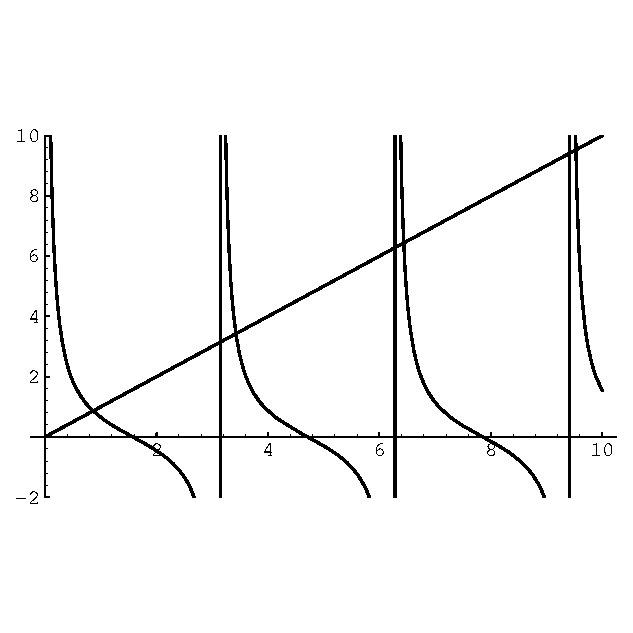
\includegraphics[height=2.5in]{pde/separation/cot}
  \end{center}
  \caption{The eigenvalues.}
  \label{cot}
\end{figure}



The solution for $\phi$ is
\[ \phi_n = a_n \cos(\sqrt{\lambda_n} t) + b_n \sin(\sqrt{\lambda_n} t). \]
Thus the solution to the differential equation is
\[ u(x,t) = \sum_{n=1}^\infty \cos(\sqrt{\lambda_n} x) [a_n \cos(\sqrt{\lambda_n}t)
+ b_n \sin(\sqrt{\lambda_n} t)]. \]

Let
\begin{align*}
  f(x) &= \sum_{n=1}^\infty f_n \cos(\sqrt{\lambda_n} x) \\
  g(x) &= \sum_{n=1}^\infty g_n \cos(\sqrt{\lambda_n} x).
\end{align*}
From the initial value we have
\begin{gather*}
  \sum_{n=1}^\infty \cos(\sqrt{\lambda_n x})a_n = \sum_{n=1}^\infty f_n \cos(\sqrt{\lambda_n}x)\\
  a_n = f_n.
\end{gather*}
The initial velocity condition gives us
\begin{gather*}
  \sum_{n=1}^\infty \cos(\sqrt{\lambda_n} x) \sqrt{\lambda_n} b_n =
  \sum_{n=1}^\infty g_n \cos(\sqrt{\lambda_n}x) \\
  b_n = \frac{g_n}{\sqrt{\lambda_n}}.
\end{gather*}

Thus the solution is
\[ \boxed{ u(x,t) = \sum_{n=1}^\infty \cos(\sqrt{\lambda_n}x)
  \left[f_n \cos(\sqrt{\lambda_n}t) + \frac{g_n}{\sqrt{\lambda_n}}
    \sin(\sqrt{\lambda_n}t)\right]. } \]






%%=============================================================================
\section{General Method}

Here is an outline detailing the method of separation of variables for
a linear partial differential equation for $u(x, y, z, \ldots)$.

\begin{enumerate}
\item
  Substitute $u(x, y, z, \ldots) = X(x) Y(y) Z(z) \cdots$ into the partial
  differential equation.  Separate the equation into ordinary differential
  equations.
\item
  Translate the boundary conditions for $u$ into boundary conditions for
  $X$, $Y$, $Z$, $\ldots$.  The continuity of $u$ may give additional boundary
  conditions and boundedness conditions.
\item
  Solve the differential equation(s) that determine the eigenvalues.
  Make sure to consider all cases.
  The eigenfunctions will be determined up to a multiplicative constant.
\item
  Solve the rest of the differential equations subject to the homogeneous
  boundary conditions.  The eigenvalues will be a parameter in the solution.
  The solutions will be determined up to a multiplicative constant.
\item
  The eigen-solutions are the product of the solutions of the ordinary
  differential equations.  $\phi_n = X_n Y_n Z_n \cdots$.
  The solution of the partial differential equation is a linear combination of
  the eigen-solutions.
  \[
  u(x,y,z,\ldots) = \sum a_n \phi_n
  \]
\item
  Solve for the coefficients, $a_n$ using the inhomogeneous boundary conditions.
\end{enumerate}




\raggedbottom
%%=============================================================================
\exercises{
\pagebreak
\flushbottom
\section{Exercises}








\begin{Exercise}
  \label{exercise heat=qxyt ab}
  Solve the following problem with separation of variables.
  \begin{gather*}
    u_t - \kappa ( u_{x x} + u_{y y} ) = q(x,y,t), \quad 0 < x < a,\ 0 < y < b
    \\
    u(x,y,0) = f(x,y), \quad u(0,y,t) = u(a,y,t) = u(x,0,t) = u(x,b,t) = 0
  \end{gather*}

  \hintsolution{heat=qxyt ab}
\end{Exercise}











\begin{Exercise}
  \label{exercise radiated half pipe}
  Consider a thin half pipe of unit radius laying on the ground.  It is heated
  by radiation from above.  We take the initial temperature of the pipe and 
  the temperature of the ground to be zero.  We model this problem with a 
  heat equation with a source term.
  \begin{gather*}
    u_t = \kappa u_{x x} + A \sin(x)
    \\
    u(0,t) = u(\pi,t) = 0, \quad u(x,0) = 0
  \end{gather*}

  \hintsolution{radiated half pipe}
\end{Exercise}




\begin{Exercise}
  \label{exercise laplace quarter circe two bc}
  Consider Laplace's Equation $\nabla^2 u = 0$ inside the quarter circle of 
  radius 1 ($0 \leq \theta \leq \frac{\pi}{2}$, $0 \leq r \leq 1$). Write the problem in 
  polar coordinates $u = u(r,\theta)$ and use separation of variables to find the 
  solution subject to the following boundary conditions.
  \begin{enumerate}
  \item 
    \[ 
    \frac{\partial u}{\partial \theta} (r,0) = 0, \quad u \left( r, \frac{\pi}{2} \right) = 0, 
    \quad u(1,\theta) = f(\theta)
    \]
  \item 
    \[ 
    \frac{\partial u}{\partial \theta} (r,0) = 0, \quad  
    \frac{\partial u}{\partial \theta} \left( r, \frac{\pi}{2} \right) = 0, 
    \quad \frac{\partial u}{\partial r}(1,\theta) = g(\theta)
    \]
    Under what conditions does this solution exist? 
  \end{enumerate}

  \hintsolution{laplace quarter circe two bc}
\end{Exercise}







\begin{Exercise}
  \label{exercise head 2D insulated fixed initial}
  Consider the 2-D heat equation
  \[ 
  u_t = \nu (u_{x x}+u_{y y}),
  \]
  on a square plate $0 < x < 1$, $0 < y < 1$ with two sides insulated
  \[ 
  u_x(0,y,t) = 0 \quad u_x(1,y,t) = 0,
  \]
  two sides with fixed temperature
  \[ 
  u(x,0,t) = 0 \quad u(x,1,t) = 0,
  \]
  and initial temperature
  \[ 
  u(x,y,0) = f(x,y).
  \]

  \begin{enumerate}
  \item 
    Reduce this to a set of 3 ordinary differential equations using 
    separation of variables. 
  \item 
    Find the corresponding set of eigenfunctions and 
    give the solution satisfying the given initial condition. 
  \end{enumerate}

  \hintsolution{head 2D insulated fixed initial}
\end{Exercise}








\begin{Exercise}
  \label{exercise ut=nuuxx ux=ux=0}
  Solve the 1-D heat equation
  \[ 
  u_t = \nu u_{x x},
  \]
  on the domain $0 < x < \pi$ subject to conditions that the ends
  are insulated (i.e. zero flux)
  \[ 
  u_x(0,t) = 0 \quad u_x(\pi,t) = 0,
  \]
  and the initial temperature distribution is $u(x,0) = x$.

  \hintsolution{ut=nuuxx ux=ux=0}
\end{Exercise}



%% Poisson's formula for a disk.
\begin{Exercise}
  \label{exercise Poisson formula for a disk}
  Obtain Poisson's formula
  to solve the Dirichlet problem for the circular region $0 \leq r < R$,
  $0 \leq \theta < 2\pi$. That is, determine a solution 
  $\phi(r,\theta)$ to Laplace's  equation
  \[
  \nabla^2 \phi  = 0
  \]
  in polar coordinates given $\phi(R,\theta)$. Show that
  \[
  \phi(r,\theta) = \frac{1}{2 \pi} \int_0^{2 \pi} \phi(R,\alpha) 
  \frac{ R^2 - r^2 }{ R^2 + r^2 - 2 R r \cos(\theta - \alpha) } 
  \,\dd \alpha
  \]

  \hintsolution{Poisson formula for a disk}
\end{Exercise}



%% Heat equation on a ring.
\begin{Exercise}
  \label{exercise Heat equation on a ring}
  Consider the temperature of a ring of unit radius.  Solve the problem
  \[
  u_t = \kappa u_{\theta\theta}, \quad u(\theta,0) = f(\theta)
  \]
  with separation of variables.

  \hintsolution{Heat equation on a ring}
\end{Exercise}




%%11111111111111111111111111111111111111111111111111111111111111111111111111111
\begin{Exercise}
  \label{exercise laplace separation 0101}
  Solve the Laplace's equation by separation of variables.
  \begin{gather*}
    \Delta u \equiv u_{x x} + u_{y y} = 0, \quad 0 < x < 1, \quad 0 < y < 1, \\
    u(x,0) = f(x), \quad u(x,1) = 0, \quad
    u(0,y) = 0, \quad u(1,y) = 0
  \end{gather*}
  Here $f(x)$ is an arbitrary function which is known.

  \hintsolution{laplace separation 0101}
\end{Exercise}






%%22222222222222222222222222222222222222222222222222222222222222222222222222222
\begin{Exercise}
  \label{exercise laplace unit disk}
  Solve Laplace's equation in the unit disk with separation of variables.
  \begin{gather*}
    \Delta u = 0, \quad 0 < r < 1
    \\
    u(1,\theta) = f(\theta)
  \end{gather*}
  The Laplacian in cirular coordinates is
  \[
  \Delta u \equiv \frac{\partial^2 u}{\partial r^2} + \frac{1}{r} \frac{\partial u}{\partial r} 
  + \frac{1}{r^2} \frac{\partial^2 u}{\partial \theta^2}.
  \]

  \hintsolution{laplace unit disk}
\end{Exercise}







%%33333333333333333333333333333333333333333333333333333333333333333333333333333
\begin{Exercise}
  \label{exercise normal modes drum unit radius}
  Find the normal modes of oscillation of a drum head of unit radius.  
  The drum head obeys the wave equation with zero displacement on the boundary.
  \[
  \Delta v \equiv \frac{1}{r} \frac{\partial}{\partial r} \left( r \frac{\partial v}{\partial r} \right)
  + \frac{1}{r^2} \frac{\partial^2 v}{\partial \theta^2} = \frac{1}{c^2} \frac{\partial^2 v}{\partial t^2}, 
  \qquad v(1,\theta,t) = 0
  \]

  \hintsolution{normal modes drum unit radius}
\end{Exercise}




%% Diffusion equation with zero boundary conditions
\begin{Exercise}
  \label{exercise diffusion equation zero bc}
  Solve the equation
  \[
  \phi_t = a^2 \phi_{x x}, \quad 0 < x < l, \quad t > 0
  \]
  with boundary conditions $\phi(0, t) = \phi(l, t) = 0$, and initial conditions
  \[
  \phi(x, 0) = \begin{cases}
    x, &0 \leq x \leq l/2, \\
    l-x, & l/2 < x \leq l.
  \end{cases}
  \]
  Comment on the differentiability ( that is the number of finite derivatives
  with respect to $x$ ) at time $t = 0$ and at time $t = \epsilon$, 
  where $\epsilon > 0$ and $\epsilon \ll 1$.

  \hintsolution{diffusion equation zero bc}
\end{Exercise}





%% Diffusion equation with nonzero boundary conditions
\begin{Exercise}
  \label{exercise diffusion nonzero bc}
  Consider a one-dimensional rod of length $L$ with initial temperature 
  distribution $f(x)$.  The temperatures at the left and right ends of the rod
  are held at $T_0$ and $T_1$, respectively.  To find the temperature of the
  rod for $t>0$, solve
  \begin{gather*}
    u_t = \kappa u_{x x}, \quad 0 < x < L, \quad t > 0 \\
    u(0,t) = T_0, \quad u(L,t) = T_1, \quad u(x,0) = f(x),
  \end{gather*}
  with separation of variables.

  \hintsolution{diffusion nonzero bc}
\end{Exercise}



%% \phi_t = a^2 \phi_{xx} + w(x,t), \phi(0,t) = 0,\quad \phi_x(l,t) = 0
\begin{Exercise}
  \label{exercise pt=a2pxx+w p=0 px=0}
  \label{phi_t=a^2phi_xx+w(x,t),phi(0,t)=0,quadphi_x(l,t)=0}
  For $ 0 < x < l$ solve the problem
  \begin{gather}
    \label{phi_t=a2phi_xx+w}
    \phi_t = a^2 \phi_{xx} + w(x,t) \\
    \nonumber
    \phi(0,t) = 0,\quad \phi_x(l,t) = 0,\quad \phi(x,0) = f(x)
  \end{gather}
  by means of a series expansion involving the eigenfunctions of
  \begin{gather*}
    \frac{\dd^2 \beta(x)}{\dd x^2} + \lambda \beta(x) = 0, \\
    \beta(0) = \beta'(l) = 0.
  \end{gather*}
  Here $w(x,t)$ and $f(x)$ are prescribed functions.

  \hintsolution{pt=a2pxx+w p=0 px=0}
\end{Exercise}





%% Heat equation, \phi(0,t) = 0, \quad c \phi(l,t) + \phi_x(l,t) = 0.
\begin{Exercise}
  \label{exercise heat p=0 cp+px=0}
  \label{Heat_equation,phi(0,t)=0,quadcphi(l,t)+phi_x(l,t)=0}
  Solve the heat equation of 
  Exercise~\ref{phi_t=a^2phi_xx+w(x,t),phi(0,t)=0,quadphi_x(l,t)=0} with the
  same initial conditions but with the boundary conditions
  \[
  \phi(0,t) = 0, \quad c \phi(l,t) + \phi_x(l,t) = 0.
  \]
  Here $c > 0$ is a constant. Although it is not possible to solve for the
  eigenvalues $\lambda$ in closed form, show that the
  eigenvalues assume a simple form for large values of $\lambda$.

  \hintsolution{heat p=0 cp+px=0}
\end{Exercise}





%% Heat equation, \phi(0,t) = t, \quad \phi_x(l,t) = - c\phi(l,t)
\begin{Exercise}
  \label{exercise heat p=t px=-cp}
  Use a series expansion technique to solve the 
  problem
  \[
  \phi_t = a^2\phi_{xx} + 1, \qquad t > 0,\quad 0 < x < l
  \]
  with boundary and initial conditions given by
  \[
  \phi(x,0) = 0, \quad \phi(0,t) = t, \quad \phi_x(l,t) = - c\phi(l,t)
  \]
  where $c > 0$ is a constant.

  \hintsolution{heat p=t px=-cp}
\end{Exercise}




%% Heat eqn.  Radiation BC.  2 series solutions.
\begin{Exercise}
  \label{exercise heat radiation bc 2 series solutions}
  Let $\phi(x,t)$ satisfy the equation 
  \[
  \phi_t = a^2\phi_{xx}
  \]
  for $0 < x< l$, $ t > 0$ with initial conditions $\phi(x,0) = 0$
  for $0 < x < l$, with boundary conditions $\phi(0,t) = 0$ for $ t >
  0$, and $\phi(l,t) + \phi_x(l,t) = 1 $ for $ t > 0$. Obtain two series
  solutions for this problem, one which is useful for large $t$ and the
  other useful for small $t$.

  \hintsolution{heat radiation bc 2 series solutions}
\end{Exercise}





%% \phi_t = A^2(x^2 \phi_x)_x, where $A$ is a  constant. 
\begin{Exercise}
  \label{exercise pt=A2x2pxx}
  A rod occupies the portion $1 < x < 2$ of 
  the x-axis. The thermal conductivity depends on $x$ in such a manner that
  the temperature $\phi(x,t)$ satisfies the equation
  \begin{equation}
    \label{phi_t=A^2x^2phi_x_x}
    \phi_t = A^2(x^2 \phi_x)_x
  \end{equation}
  where $A$ is a  constant. For $\phi(1,t) = \phi(2,t) = 0$ for $t > 0$,
  with $\phi(x,0) = f(x)$ for  $1 < x < 2$, show that the appropriate series
  expansion involves the eigenfunctions
  \[
  \beta_n(x) = \frac{1}{\sqrt{x}} \sin \left( \frac{\pi n \ln x}{\ln 2}
  \right ).
  \]
  Work out the series expansion for the given boundary and initial conditions.

  \hintsolution{pt=A2x2pxx}
\end{Exercise}






%% Wave equation with fixed and free end, zero initial velocity.
\begin{Exercise}
  \label{exercise wave fixed free end zero}
  Consider a string of length $L$ with a fixed left end a free right end.
  Initially the string is at rest with displacement $f(x)$.  Find the 
  motion of the string by solving,
  \begin{gather*}
    u_{t t} = c^2 u_{x x}, \quad 0 < x < L, \quad t > 0, \\
    u(0,t) = 0, \quad u_x(L,t) = 0, \\
    u(x,0) = f(x), \quad u_t(x,0) = 0,
  \end{gather*}
  with separation of variables.

  \hintsolution{wave fixed free end zero}
\end{Exercise}





%% Potential equation
\begin{Exercise}
  \label{exercise potential 2d block zero insulated}
  Consider the equilibrium temperature distribution in a two-dimensional 
  block of width $a$ and height $b$.  There is a heat source given by the 
  function $f(x,y)$.  The vertical sides of the block are held at zero 
  temperature; the horizontal sides are insulated.
  To find this equilibrium temperature distribution, solve the potential 
  equation,
  \begin{gather*}
    u_{x x} + u_{y y} = f(x, y), \quad 0 < x < a, \quad 0 < y < b, \\
    u(0,y) = u(a,y) = 0, \quad u_y(x,0) = u_y(x,b) = 0,
  \end{gather*}
  with separation of variables.

  \hintsolution{potential 2d block zero insulated}
\end{Exercise}







%% Vibrations of a beam.
\begin{Exercise}
  \label{exercise vibrations of a beam}
  Consider the vibrations of a stiff beam of length $L$.  More precisely, 
  consider the transverse vibrations of an unloaded beam, whose weight can be 
  neglected compared to its stiffness.  The beam is simply supported at 
  $x = 0,L$. (That is, it is resting on fulcrums there.  $u(0,t) = 0$ means 
  that the beam is resting on the fulcrum; $u_{x x}(0,t) = 0$ indicates that
  there is no bending force at that point.)  The beam has initial displacement 
  $f(x)$ and velocity $g(x)$.  To determine the motion of the beam, solve
  \begin{gather*}
    u_{t t} + a^2 u_{x x x x} = 0, \quad 0 < x < L, \quad t > 0, \\
    u(x,0) = f(x), \quad u_t(x,0) = g(x), \\
    u(0,t) = u_{x x}(0,t) = 0, \quad u(L,t) = u_{x x}(L,t) = 0, 
  \end{gather*}
  with separation of variables.

  \hintsolution{vibrations of a beam}
\end{Exercise}



%% Magnet winding
\begin{Exercise}
  \label{exercise magnet winding}
  The temperature along a magnet winding of length $L$ carrying a current $I$
  satisfies, (for some $\alpha > 0$):
  \[
  u_t = \kappa u_{x x} + I^2 \alpha u.
  \]
  The ends of the winding are kept at zero, i.e.,
  \[
  u(0,t) = u(L,t) = 0;
  \]
  and the initial temperature distribution is
  \[
  u(x,0) = g(x).
  \]
  Find $u(x,t)$ and determine the critical current $I_{CR}$ which is defined
  as the least current at which the winding begins to heat up exponentially.
  Suppose that $\alpha < 0$, so that the winding has a negative coefficient
  of resistance with respect to temperature.  What can you say about the
  critical current in this case?

  \hintsolution{magnet winding}
\end{Exercise}



%% e-folding time
\begin{Exercise}
  \label{exercise e-folding time}
  The "e-folding" time of a decaying function of time is the time interval,
  $\Delta_e$, in which the magnitude of the function is reduced by at least
  $\frac{1}{e}$.  Thus if $u(x,t) = \e^{-\alpha t} f(x) + \e^{-\beta t} g(x)$
  with $\alpha > \beta > 0$ then $\Delta_e = \frac{1}{\beta}$.  A body
  with heat conductivity $\kappa$ has its exterior surface maintained at
  temperature zero.  Initially the interior of the body is at the uniform
  temperature $T > 0$.  Find the e-folding time of the body if it is:
  \begin{itemize}
    %%
  \item[a)]
    An infinite slab of thickness $a$.
    %%
  \item[b)]
    An infinite cylinder of radius $a$.
    %%
  \item[c)]
    A sphere of radius $a$.
  \end{itemize}
  Note that in (a) the temperature varies only in the $z$ direction and in time;
  in (b) and (c) the temperature varies only in the radial direction
  and in time.  

  \begin{itemize}
    %%
  \item[d)]
    What are the e-folding times if the surfaces are perfectly insulated, 
    (i.e., $\frac{\partial u}{\partial n} = 0$, where $n$ is the exterior normal at the 
    surface)? 
  \end{itemize}

  \hintsolution{e-folding time}
\end{Exercise}





%% Heat equation in rectangle with non-constant diffusivity.
\begin{Exercise}
  \label{exercise heat rectangle non-constant diffusivity}
  Solve the heat equation with a time-dependent diffusivity in the rectangle
  $0 < x < a$, $0 < y < b$.  The top and bottom sides are held at temperature
  zero; the lateral sides are insulated.
  We have the initial-boundary value problem:
  \begin{gather*}
    u_t = \kappa(t) \left( u_{x x} + u_{y y} \right), \quad
    0 < x < a, \quad 0 < y < b, \quad t > 0, \\
    u(x,0,t) = u(x,b,t) = 0, \\
    u_x(0,y,t) = u_x(a,y,t) = 0, \\
    u(x,y,0) = f(x,y).
  \end{gather*}
  The diffusivity, $\kappa(t)$, is a known, positive function.

  \hintsolution{heat rectangle non-constant diffusivity}
\end{Exercise}



%% semi-circular rod
\begin{Exercise}
  \label{exercise potential semi-circular rod}
  A semi-circular rod of infinite extent is maintained at temperature $T = 0$
  on the flat side and at $T = 1$ on the curved surface:
  \[
  x^2 + y^2 = 1, \quad y > 0.
  \]
  Find the steady state temperature in a cross section of the rod using
  separation of variables.

  \hintsolution{potential semi-circular rod}
\end{Exercise}


%% Steady state temperature in a semi-infinite rectangular slab.
\begin{Exercise}
  \label{exercise heat semi-infinite rectangular slab}
  Use separation of variables to find the steady state temperature 
  $u(x,y)$ in a slab: $x \geq 0$, 
  $0 \leq y \leq 1$, which has zero temperature on the faces $y = 0$ and
  $y = 1$ and has a given distribution: $u(y,0) = f(y)$ on the 
  edge $x = 0$, $0 \leq y \leq 1$.

  \hintsolution{heat semi-infinite rectangular slab}
\end{Exercise}



%% Harmonic function in a sector with one inhomogeneous boundary condition.
\begin{Exercise}
  \label{exercise harmonic sector inhomogeneous bc}
  Find the solution of Laplace's equation subject to the boundary conditions.
  \begin{gather*}
    \Delta u = 0, \quad 0 < \theta < \alpha, \quad a < r < b,
    \\
    u(r,0) = u(r,\alpha) = 0, \quad u(a,\theta) = 0, \quad u(b,\theta) = f(\theta).
  \end{gather*}

  \hintsolution{harmonic sector inhomogeneous bc}
\end{Exercise}







%% Piano string instantaneously struck.
\begin{Exercise}
  \label{exercise piano string instantaneously struck}
  $\phantom{a}$

  \textbf{a)}
  A piano string of length $L$ is struck, at time $t = 0$, by a flat hammer of
  width $2 d$ centered at a point $\xi$, having velocity $v$.  Find the ensuing
  motion, $u(x, t)$, of the string for which the wave speed is $c$.

  \textbf{b)}
  Suppose the hammer is curved, rather than flat as above, so that the initial 
  velocity distribution is
  \[
  u_t(x, 0) = 
  \begin{cases}
    v \cos \left( \frac{\pi(x-\xi)}{2d} \right), &|x-\xi| < d \\
    0 &|x-\xi| > d.
  \end{cases}
  \]
  Find the ensuing motion.

  \textbf{c)}
  Compare the kinetic energies of each harmonic in the two solutions.  Where 
  should the string be struck in order to maximize the energy in the 
  $n^{\mathrm{th}}$ harmonic in each case?

  %% CONTINUE  Make predictions based on the physics.

  \hintsolution{piano string instantaneously struck}
\end{Exercise}







%% Piano string, time dependent forcing.
\begin{Exercise}
  \label{exercise piano string time dependent forcing}
  If the striking hammer is not perfectly rigid, then its effect must be 
  included as a time dependent forcing term of the form:
  \[
  s(x, t) = \begin{cases}
    v \cos\left( \frac{\pi(x-\xi)}{2d} \right) 
    \sin\left( \frac{\pi t}{\delta} \right),
    &\mathrm{for}\ |x-\xi| < d, \quad 0 < t < \delta, \\
    0 &\mathrm{otherwise}.
  \end{cases}
  \]
  Find the motion of the string for $t > \delta$.  Discuss the effects of the
  width of the hammer and duration of the blow with regard to the energy
  in overtones.

  \hintsolution{piano string time dependent forcing}
\end{Exercise}





%% Propagating modes of a square waveguide.
\begin{Exercise}
  \label{exercise propagating modes square waveguide}
  Find the propagating modes in a square waveguide of side $L$ for harmonic
  signals of frequency $\omega$ when the propagation speed of the medium
  is $c$.  That is, we seek those solutions of 
  \[
  u_{t t} - c^2 \Delta u = 0,
  \]
  where $u = u(x, y, z, t)$ has the form 
  $u(x, y, z, t) = v(x, y, z) \e^{\imath \omega t}$, which satisfy the conditions:
  \begin{gather*}
    u(x, y, z, t) = 0 \quad \mathrm{for} \quad x = 0,L, \quad y = 0,L, \quad z > 0,\\
    \lim_{z \to \infty} |u| \neq \infty\ \mathrm{and}\ \neq 0.
  \end{gather*}
  Indicate in terms of inequalities involving $k = \omega / c$ and appropriate
  eigenvalues, $\lambda_{n,m}$ say, for which $n$ and $m$ the solutions
  $u_{n,m}$ satisfy the conditions.
  %% CONTINUE: perhaps improve wording.

  \hintsolution{propagating modes square waveguide}
\end{Exercise}




%% Rectangular drum head.  Modes of oscillation.
\begin{Exercise}
  \label{exercise rectangular drum head modes}
  Find the modes of oscillation and their frequencies for a rectangular 
  drum head of width $a$ and height $b$.  The modes of oscillation are 
  eigensolutions of
  \begin{gather*}
    u_{t t} = c^2 \Delta u, \quad 0 < x < a,\ 0 < y < b, \\
    u(0,y) = u(a,y) = u(x,0) = u(x,b) = 0.
  \end{gather*}

  \hintsolution{rectangular drum head modes}
\end{Exercise}




%% \phi_t = a^2\left(\phi_{xx} + \phi_{yy}\right)
\begin{Exercise}
  \label{exercise separation pt=a2pxx+pyy}
  Using separation of variables solve the heat equation
  \[
  \phi_t = a^2\left(\phi_{xx} + \phi_{yy}\right)
  \]
  in the rectangle $0 < x < l_x$, $0 < y < l_y$ with initial conditions
  \[
  \phi(x,y,0) = 1,
  \]
  and boundary conditions
  \[
  \phi(0,y,t) = \phi(l_x,y,t) = 0,\quad
  \phi_y(x,0,t) = \phi_y(x,l_y,t) = 0.
  \]

  \hintsolution{separation pt=a2pxx+pyy}
\end{Exercise}






%% Using polar coordinates and separation of variables solve the heat equation.
\begin{Exercise}
  \label{exercise heat polar separation}
  Using polar coordinates and separation of variables
  solve the heat equation
  \[
  \phi_t = a^2 \nabla^2 \phi
  \]
  in the circle $0 < r < R_0$ with initial conditions
  \[
  \phi(r,\theta,0) = V
  \]
  where $V$ is a constant, and boundary conditions
  \[
  \phi(R_0,\theta,t) = 0.  
  \]
  \begin{enumerate}
  \item Show that for $t > 0$,
    \[
    \phi(r,\theta,t) = 2V \sum_{n=1}^\infty
    \exp\left(- \frac{a^2 j_{0,n}^2}{R_0^2} t \right) 
    \frac{ J_0\left({j_{0,n} r  / R_0}\right)}
    {j_{0,n} J_1(j_{0,n})},
    \]
    where $j_{0,n}$ are the roots of $J_0(x)$:
    \begin{displaymath}
      J_0(j_{0,n}) = 0,\quad n = 1,2,\ldots
    \end{displaymath}
    {\it Hint: The following identities may be of some help:}
    \begin{displaymath}
      \begin{array}{ll}
        \rule[-3mm]{0mm}{10mm}\displaystyle \int_0^{R_0} r
        J_0\left({j_{0,n}r / R_0}\right) 
        J_0\left({j_{0,m}r / R_0}\right)dr = 0, &\quad m \neq n, \\
        \rule[-3mm]{0mm}{10mm}\displaystyle \int_0^{R_0} r
        J_0^2\left({j_{0,n}r / R_0}\right) dr = \frac{R_0^2}{2}
        J_1^2(j_{0,n}), & \\ 
        \rule[-3mm]{0mm}{10mm}\displaystyle \int_0^r r J_0(\beta r) dr
        = \frac{r}{\beta} J_1(\beta r)&\quad {\rm for~any~}\beta.\\ 
      \end{array}
    \end{displaymath}
  \item For any fixed $r$, $0 < r < R_0$, use the asymptotic approximation
    for the $J_n$ Bessel functions for large argument (this can be found
    %% CONTINUE: make sure this is in the appendices
    in any standard math tables) to
    determine the rate of decay of the terms of the series solution for
    $\phi$ at time $ t = 0$. 
  \end{enumerate}

  \hintsolution{heat polar separation}
\end{Exercise}






%% Consider the solution of the diffusion equation in spherical coordinates.
\begin{Exercise}
  \label{exercise diffusion spherical separation}
  Consider the solution of the diffusion
  equation in spherical coordinates given by
  \begin{eqnarray*}
    x &=& r \sin \theta \cos \phi, \\
    y &=& r \sin \theta \sin \phi, \\
    z &=& r \cos \theta,
  \end{eqnarray*}
  where $r$ is the radius, $\theta$ is the polar angle, and $\phi$ is
  the azimuthal angle. 
  We wish to solve the equation on the {\bf surface} of the sphere given 
  by $ r = R$, $ 0 < \theta < \pi$, and $ 0 < \phi < 2\pi$.  The
  diffusion equation for the solution $\Psi(\theta,\phi,t)$ 
  in these coordinates on the surface of the sphere becomes
  \begin{equation}
    \label{fpdfracPsit=fraca^2R^2left(frac1sintheta}
    \frac{\partial \Psi}{\partial t} = \frac{a^2}{R^2} \left( \frac{1}{\sin \theta}
      \frac{\partial}{\partial \theta} \left( \sin \theta \frac{\partial \Psi}{\partial \theta} \right) 
      + \frac{1}{\sin^2 \theta} \frac{\partial^2 \Psi}{\partial \phi^2} \right).
  \end{equation}
  where  $a$ is a positive constant.
  \begin{enumerate}
  \item Using separation of variables show that a solution
    $\Psi$ can be found in the form
    \begin{displaymath}
      \Psi(\theta,\phi,t) = T(t) \Theta(\theta) \Phi(\phi),
    \end{displaymath}
    where $T$,$\Theta$,$\Phi$ obey ordinary differential equations
    in $t$,$\theta$, and $\phi$ respectively. 
    Derive the ordinary differential equations
    for $T$ and $\Theta$, and 
    show that  the differential equation obeyed by $\Phi$ is given by
    \begin{displaymath}
      \frac{\dd^2 \Phi}{\dd \phi^2} - c \Phi = 0,
    \end{displaymath}
    where $c$ is a constant.
  \item Assuming that $\Psi(\theta,\phi,t)$ is determined over the 
    full range of the azimuthal angle, $ 0 < \phi < 2\pi$, determine the 
    allowable values of the separation constant $c$ and the corresponding
    allowable functions $\Phi$. Using these values of $c$ and letting
    $x = \cos \theta$ rewrite in terms of the variable $x$ the differential
    equation satisfied by $\Theta$. What are appropriate
    boundary conditions for $\Theta$? The resulting equation is known as 
    the generalized or associated Legendre equation.
  \item Assume next that the initial conditions for $\Psi$ are
    chosen such that
    \begin{displaymath}
      \Psi(\theta,\phi,t=0) = f(\theta),
    \end{displaymath}
    where $f(\theta)$ is a specified function which is regular at
    the north and south poles (that is $\theta = 0$ and $ \theta = \pi$).
    Note that the initial condition is independent
    of the azimuthal angle $\phi$. Show that in this case the method of
    separation of variables gives a series solution for $\Psi$ of the 
    form
    \begin{displaymath}
      \Psi(\theta,t) = \sum_{l=0}^{\infty} A_l \exp(-\lambda_l^2 t) P_l(\cos\theta),
    \end{displaymath}
    where $P_l(x)$ is the $l$'th Legendre polynomial, and determine
    the constants $\lambda_l$ as a function of the index $l$.
  \item Solve for $\Psi(\theta,t)$, $ t > 0$ given that
    $f(\theta) = 2\cos^2\theta- 1$.
  \end{enumerate}
  \noindent{\it Useful facts:}
  \begin{displaymath}
    \frac{\dd}{\dd x} \left[(1-x^2) \frac{\dd P_l(x)}{\dd x}\right] + l(l+1)P_l(x) = 0
  \end{displaymath}
  \begin{eqnarray*}
    P_0(x) &=& 1 \\
    P_1(x) &=& x \\
    P_2(x) &=& \frac{3}{2}x^2 - \frac{1}{2}
  \end{eqnarray*}
  \begin{displaymath}
    \int_{-1}^1 dx P_l(x) P_m(x) = 
    \left\{
      \begin{array}{ll}
        0 \qquad &{\rm if~} l\neq m \\
        \displaystyle \frac{2}{2l+1}\qquad &{\rm if~} l = m \\
      \end{array}
    \right.
  \end{displaymath}

  \hintsolution{diffusion spherical separation}
\end{Exercise}





%% Laplace's equation: with about 1\% (also 0.1\%) accuracy.
\begin{Exercise}
  \label{exercise laplace 1 percent}
  Let $\phi(x,y)$ satisfy Laplace's equation
  \[
  \phi_{xx} + \phi_{yy} = 0    
  \]
  in the rectangle $0 < x < 1$, $0 < y < 2$, with $\phi(x,2) = x(1-x)$, and
  with $\phi = 0$ on the other three sides. Use a series solution to determine
  $\phi$ inside the rectangle. How many terms are required to give
  $\phi(\frac{1}{2},1)$ with about 1\% (also 0.1\%) accuracy; how about
  $\phi_x(\frac{1}{2},1)$?

  \hintsolution{laplace 1 percent}
\end{Exercise}








%% Laplace's equation: spherical coordinates, two regions.
\begin{Exercise}
  \label{exercise laplace spherical two regions}
  Let $\psi(r,\theta,\phi)$ satisfy
  Laplace's equation in spherical coordinates in each of the two regions
  $r < a$, $r > a$, with $ \psi \to 0$ as $ r \to \infty$. Let
  \begin{align*}
    \lim_{r\to a^+} \psi (r,\theta,\phi) - \lim_{r\to a^-} \psi (r,\theta,\phi) 
    &= 0,\\
    \lim_{r\to a^+} \psi_r (r,\theta,\phi) - 
    \lim_{r\to a^-} \psi_r (r,\theta,\phi) &= P_n^m (\cos \theta) 
    \sin(m \phi),
  \end{align*}
  where $m$ and $n \geq m$ are integers. Find $\psi$ in $r < a$ and $r > a$. In
  electrostatics, this problem corresponds to that of determining the potential
  of a spherical harmonic 
  type charge distribution over the surface of the sphere.
  In this way one can determine the potential due to an arbitrary surface
  charge distribution since any charge distribution can be expressed as a series
  of spherical harmonics.

  \hintsolution{laplace spherical two regions}
\end{Exercise}








%% Obtain a formula analogous to the Poisson formula to solve Neumann problem.
\begin{Exercise}
  \label{exercise poisson formula neumann}
  Obtain a formula analogous to the Poisson formula
  to solve the Neumann problem for the circular region $0 \leq r < R$,
  $0 \leq \theta < 2\pi$. That is, determine a solution 
  $\phi(r,\theta)$ to Laplace's  equation
  \[
  \nabla^2 \phi  = 0
  \]
  in polar coordinates given $\phi_r(R,\theta)$. Show that
  \[
  \phi (r,\theta) = - \frac{R}{2 \pi} \int_0^{2\pi}
  \phi_r(R,\alpha)\ln\left[ 1 - \frac{2r}{R}\cos(\theta -\alpha) + 
    \frac{r^2}{R^2}\right] \,\dd \alpha
  \]
  within an arbitrary additive constant.

  \hintsolution{poisson formula neumann}
\end{Exercise}






%% Investigate solutions of \[\phi_t = a^2 \phi_{x x}\]
\begin{Exercise}
  \label{exercise separation pt=a2pxx}
  Investigate solutions of 
  \[
  \phi_t = a^2 \phi_{x x}
  \]
  obtained by setting the separation constant $C = (\alpha + \imath \beta)^2$
  in the equations obtained by assuming $\phi = X(x) T(t)$:
  \[
  \frac{T'}{T} = C, \quad
  \frac{X''}{X} = \frac{C}{a^2}.
  \]

  \hintsolution{separation pt=a2pxx}
\end{Exercise}










\raggedbottom
}
%%=============================================================================
\hints{
\pagebreak
\flushbottom
\section{Hints}




\begin{Hint}
  \label{hint heat=qxyt ab}
  %% CONTINUE
\end{Hint}




\begin{Hint}
  \label{hint radiated half pipe}
  %% CONTINUE
\end{Hint}




\begin{Hint}
  \label{hint laplace quarter circe two bc}
  %% CONTINUE
\end{Hint}




\begin{Hint}
  \label{hint head 2D insulated fixed initial}
  %% CONTINUE
\end{Hint}




\begin{Hint}
  \label{hint ut=nuuxx ux=ux=0}
  %% CONTINUE
\end{Hint}




%% Poisson's formula for a disk.
\begin{Hint}
  \label{hint Poisson formula for a disk}
  %% CONTINUE
\end{Hint}




%% Heat equation on a ring.
\begin{Hint}
  \label{hint Heat equation on a ring}
  Impose the boundary conditions
  \[
  u(0,t) = u(2 \pi,t), \quad
  u_\theta(0,t) = u_\theta(2 \pi,t).
  \]
\end{Hint}





%%111
\begin{Hint}
  \label{hint laplace separation 0101}
  Apply the separation of variables $u(x,y) = X(x) Y(y)$.
  Solve an eigenvalue problem for $X(x)$.
\end{Hint}

%%222
\begin{Hint}
  \label{hint laplace unit disk}
  %% CONTINUE
\end{Hint}

%%333
\begin{Hint}
  \label{hint normal modes drum unit radius}
  %% CONTINUE
\end{Hint}

%% Diffusion equation with zero boundary conditions
\begin{Hint}
  \label{hint diffusion equation zero bc}
  %% CONTINUE
\end{Hint}


%% Diffusion equation with nonzero boundary conditions
\begin{Hint}
  \label{hint diffusion nonzero bc}
  There are two ways to solve the problem.  For the first method, 
  expand the solution in a series of the form
  \[
  u(x,t) = \sum_{n=1}^\infty a_n(t) \sin \left( \frac{n \pi x}{L} \right).
  \]
  Because of the inhomogeneous boundary conditions, the convergence of 
  the series will not be uniform.  You can differentiate the series with
  respect to $t$, but not with respect to $x$.  Multiply the partial
  differential equation by the eigenfunction $\sin(n \pi x / L)$ and 
  integrate from $x=0$ to $x=L$.  Use integration by parts to move derivatives
  in $x$ from $u$ to the eigenfunctions.  This process will yield a 
  first order, ordinary differential equation for each of the $a_n$'s.

  For the second method:
  Make the change of variables $v(x,t) = u(x,t) - \mu(x)$, where $\mu(x)$
  is the equilibrium temperature distribution to obtain a problem with 
  homogeneous boundary conditions.  
\end{Hint}



%% \phi_t = a^2 \phi_{xx} + w(x,t), \phi(0,t) = 0,\quad \phi_x(l,t) = 0
\begin{Hint}
  \label{hint pt=a2pxx+w p=0 px=0}
  %% CONTINUE
\end{Hint}





%% Heat equation, \phi(0,t) = 0, \quad c \phi(l,t) + \phi_x(l,t) = 0.
\begin{Hint}
  \label{hint heat p=0 cp+px=0}
  %% CONTINUE
\end{Hint}





%% Heat equation, \phi(0,t) = t, \quad \phi_x(l,t) = - c\phi(l,t)
\begin{Hint}
  \label{hint heat p=t px=-cp}
  %% CONTINUE
\end{Hint}






%% Heat eqn.  Radiation BC.  2 series solutions.
\begin{Hint}
  \label{hint heat radiation bc 2 series solutions}
  %% CONTINUE
\end{Hint}





%% \phi_t = A^2(x^2 \phi_x)_x, where $A$ is a  constant. 
\begin{Hint}
  \label{hint pt=A2x2pxx}
  %% CONTINUE
\end{Hint}



%% Wave equation with fixed and free end, zero initial velocity.
\begin{Hint}
  \label{hint wave fixed free end zero}
  Use separation of variables to find eigen-solutions of the partial differential
  equation that satisfy the homogeneous boundary conditions.  There will
  be two eigen-solutions for each eigenvalue.  Expand $u(x,t)$ in a series
  of the eigen-solutions.  Use the two initial conditions to determine the
  constants.
\end{Hint}



%% Potential equation
\begin{Hint}
  \label{hint potential 2d block zero insulated}
  Expand the solution in a series of eigenfunctions in $x$.  Determine these
  eigenfunctions by using separation of variables on the homogeneous 
  partial differential equation.   You will find that the answer has the form,
  \[
  u(x,y) = \sum_{n=1}^\infty u_n(y) \sin \left( \frac{n \pi x}{a} \right).
  \]
  Substitute this series into the partial differential equation to determine
  ordinary differential equations for each of the $u_n$'s.  The boundary
  conditions on $u(x,y)$ will give you boundary conditions for the $u_n$'s.
  Solve these ordinary differential equations with Green functions.
\end{Hint}







%% Vibrations of a beam.
\begin{Hint}
  \label{hint vibrations of a beam}
  Solve this problem by expanding the solution in a series of 
  eigen-solutions that satisfy the partial differential equation and the 
  homogeneous boundary conditions.  Use the initial conditions
  to determine the coefficients in the expansion.
\end{Hint}


%% Magnet winding
\begin{Hint}
  \label{hint magnet winding}
  Use separation of variables to find eigen-solutions that satisfy the partial
  differential equation and the homogeneous boundary conditions.  The solution
  is a linear combination of the eigen-solutions.  The whole solution will 
  be exponentially decaying if each of the eigen-solutions is exponentially
  decaying.
\end{Hint}





%% e-folding time
\begin{Hint}
  \label{hint e-folding time}
  For parts (a), (b) and (c) use separation of variables.  
  For part (b) the eigen-solutions will involve Bessel functions.  
  For part (c) the eigen-solutions will involve spherical Bessel functions.
  Part (d) is trivial.
\end{Hint}



%% Heat equation in rectangle with non-constant diffusivity.
\begin{Hint}
  \label{hint heat rectangle non-constant diffusivity}
  The solution is a linear combination of eigen-solutions of the partial 
  differential equation that satisfy the homogeneous boundary conditions.
  Determine the coefficients in the expansion with the initial condition.
\end{Hint}





%% semi-circular rod
\begin{Hint}
  \label{hint potential semi-circular rod}
  The problem is
  \begin{gather*}
    u_{r r} + \frac{1}{r} u_r + \frac{1}{r^2} 
    u_{\theta\theta} = 0, \quad 0 < r < 1, \quad 0 < \theta < \pi \\
    u(r,0) = u(r,\pi) = 0, \quad u(0,\theta) = 0, \quad u(1,\theta) = 1
  \end{gather*}
  The solution is a linear combination of eigen-solutions that satisfy the
  partial differential equation and the three homogeneous boundary conditions.
\end{Hint}





%% Steady state temperature in a semi-infinite rectangular slab.
\begin{Hint}
  \label{hint heat semi-infinite rectangular slab}
  %% CONTINUE
\end{Hint}



%% Harmonic function in a sector with one inhomogeneous boundary condition.
\begin{Hint}
  \label{hint harmonic sector inhomogeneous bc}
  %% CONTINUE
\end{Hint}





%% Piano string instantaneously struck.
\begin{Hint}
  \label{hint piano string instantaneously struck}
  %% CONTINUE
\end{Hint}






%% Piano string, time dependent forcing.
\begin{Hint}
  \label{hint piano string time dependent forcing}
  %% CONTINUE
\end{Hint}




%% Propagating modes of a square waveguide.
\begin{Hint}
  \label{hint propagating modes square waveguide}
  %% CONTINUE
\end{Hint}



%% Rectangular drum head.  Modes of oscillation.
\begin{Hint}
  \label{hint rectangular drum head modes}
  %% CONTINUE
\end{Hint}







%% \phi_t = a^2\left(\phi_{xx} + \phi_{yy}\right)
\begin{Hint}
  \label{hint separation pt=a2pxx+pyy}
  %% CONTINUE
\end{Hint}







%% Using polar coordinates and separation of variables solve the heat equation.
\begin{Hint}
  \label{hint heat polar separation}
  %% CONTINUE
\end{Hint}







%% Consider the solution of the diffusion equation in spherical coordinates.
\begin{Hint}
  \label{hint diffusion spherical separation}
  %% CONTINUE
\end{Hint}






%% Laplace's equation: with about 1\% (also 0.1\%) accuracy.
\begin{Hint}
  \label{hint laplace 1 percent}
  %% CONTINUE
\end{Hint}





%% Laplace's equation: spherical coordinates, two regions.
\begin{Hint}
  \label{hint laplace spherical two regions}
  %% CONTINUE
\end{Hint}





%% Obtain a formula analogous to the Poisson formula to solve Neumann problem.
\begin{Hint}
  \label{hint poisson formula neumann}
  %% CONTINUE
\end{Hint}






%% Investigate solutions of \[\phi_t = a^2 \phi_{x x}\]
\begin{Hint}
  \label{hint separation pt=a2pxx}
  %% CONTINUE
\end{Hint}








\raggedbottom
}
%%=============================================================================
\solutions{
\pagebreak
\flushbottom
\section{Solutions}





\begin{Solution}
  \label{solution heat=qxyt ab}
  We expand the solution in eigenfunctions in $x$ and $y$ which satify the 
  boundary conditions.
  \[
  u = \sum_{m,n = 1}^\infty u_{mn}(t) \sin \left( \frac{m \pi x}{a} \right)
  \sin \left( \frac{n \pi y}{b} \right)
  \]
  We expand the inhomogeneities in the eigenfunctions.
  \begin{gather*}
    q(x,y,t) = \sum_{m,n = 1}^\infty q_{mn}(t) \sin \left( \frac{m \pi x}{a} \right)
    \sin \left( \frac{n \pi y}{b} \right)
    \\
    q_{mn}(t) = \frac{4}{a b} \int_0^a \int_0^b q(x,y,t) \sin \left( \frac{m \pi x}{a} \right)
    \sin \left( \frac{n \pi y}{b} \right) \,\dd y \,\dd x
    \\
    f(x,y) = \sum_{m,n = 1}^\infty f_{mn} \sin \left( \frac{m \pi x}{a} \right)
    \sin \left( \frac{n \pi y}{b} \right)
    \\
    f_{mn} = \frac{4}{a b} \int_0^a \int_0^b f(x,y) \sin \left( \frac{m \pi x}{a} \right)
    \sin \left( \frac{n \pi y}{b} \right) \,\dd y \,\dd x
  \end{gather*}
  We substitute the expansion of the solution into the diffusion equation and
  the initial condition to determine initial value problems for the coefficients
  in the expansion.
  \begin{gather*}
    u_t - \kappa ( u_{x x} + u_{y y} ) = q(x,y,t)
    \\
    \sum_{m,n = 1}^\infty \left( u_{mn}'(t) + \kappa \left( \left(  \frac{m \pi}{a} \right)^2 + 
        \left( \frac{n \pi}{b} \right)^2 \right) u_{mn}(t) \right)
    \sin \left( \frac{m \pi x}{a} \right) \sin \left( \frac{n \pi y}{b} \right)
    = \sum_{m,n = 1}^\infty q_{mn}(t) \sin \left( \frac{m \pi x}{a} \right)
    \sin \left( \frac{n \pi y}{b} \right)
    \\
    u_{mn}'(t) + \kappa \left( \left( \frac{m \pi}{a} \right)^2 + 
      \left( \frac{n \pi}{b} \right)^2 \right) u_{mn}(t)
    = q_{mn}(t)
    \\
    u(x,y,0) = f(x,y)
    \\
    \sum_{m,n = 1}^\infty u_{mn}(0) \sin \left( \frac{m \pi x}{a} \right)
    \sin \left( \frac{n \pi y}{b} \right)
    = \sum_{m,n = 1}^\infty f_{mn} \sin \left( \frac{m \pi x}{a} \right)
    \sin \left( \frac{n \pi y}{b} \right)
    \\
    u_{mn}(0) = f_{mn}
  \end{gather*}
  We solve the ordinary differential equations for the coefficients $u_{mn}(t)$
  subject to their initial conditions.
  \[
  u_{mn}(t) = 
  \int_0^t \exp \left( - \kappa \left( \left( \frac{m \pi}{a} \right)^2 + 
      \left( \frac{n \pi}{b} \right)^2 \right) (t - \tau) \right) q_{mn}(\tau) \,\dd \tau
  + f_{mn} \exp \left( - \kappa \left( \left( \frac{m \pi}{a} \right)^2 + 
      \left( \frac{n \pi}{b} \right)^2 \right) t \right)
  \]
\end{Solution}









\begin{Solution}
  \label{solution radiated half pipe}
  After looking at this problem for a minute or two, it seems like the answer
  would have the form
  \[
  u = \sin(x) T(t).
  \]
  This form satisfies the boundary conditions.  We substitute it into 
  the heat equation and the initial condition to determine $T$
  \begin{gather*}
    \sin(x) T' = - \kappa \sin(x) T + A \sin(x), \quad T(0) = 0
    \\
    T' + \kappa T = A, \quad T(0) = 0
    \\
    T = \frac{A}{\kappa} + c \e^{-\kappa t}
    \\
    T = \frac{A}{\kappa} \left(1 - \e^{-\kappa t} \right)
  \end{gather*}
  Now we have the solution of the heat equation.
  \[
  u = \frac{A}{\kappa} \sin(x) \left(1 - \e^{-\kappa t} \right)
  \]
\end{Solution}






\begin{Solution}
  \label{solution laplace quarter circe two bc}
  First we write the Laplacian in polar coordinates.
  \[
  u_{r r} + \frac{1}{r} u_r + \frac{1}{r^2} u_{\theta \theta} = 0
  \]
  \begin{enumerate}
  \item
    We introduce the separation of variables $u(r, \theta) = R(r) \Theta(\theta)$.
    \begin{gather*}
      R'' \Theta + \frac{1}{r} R' \Theta + \frac{1}{r^2} R \Theta'' = 0
      \\
      r^2 \frac{R''}{R} + r \frac{R'}{R} = - \frac{\Theta''}{\Theta} = \lambda
    \end{gather*}
    We have a regular Sturm-Liouville problem for $\Theta$ and a differential 
    equation for $R$.
    \begin{gather}
      \label{eqn T''+lT=0, T'=T=0}
      \Theta'' + \lambda \Theta = 0, \quad \Theta'(0) = \Theta(\pi/2) = 0
      \\
      \nonumber
      r^2 R'' + r R' - \lambda R = 0, \quad R\ \mathrm{is bounded}
    \end{gather}

    First we solve the problem for $\Theta$ to determine the eigenvalues and
    eigenfunctions.  The Rayleigh quotient is
    \[
    \lambda = \frac{ \int_0^{\pi/2} \left( \Theta' \right)^2 \,\dd \theta }{ \int_0^{\pi/2} \Theta^2 \,\dd \theta }
    \]
    Immediately we see that the eigenvalues are non-negative.  If $\Theta' = 0$, 
    then the right boundary condition implies that $\Theta = 0$.  Thus $\lambda = 0$ is 
    not an eigenvalue.  We find the general solution of 
    Equation~\ref{eqn T''+lT=0, T'=T=0} for positive $\lambda$.
    \[
    \Theta = c_1 \cos \left( \sqrt{\lambda} \theta \right) + c_2 \sin \left( \sqrt{\lambda} \theta \right)
    \]
    The solution that satisfies the left boundary condition is
    \[
    \Theta = c \cos \left( \sqrt{\lambda} \theta \right).
    \]
    We apply the right boundary condition to determine the eigenvalues.
    \begin{gather*}
      \cos \left( \sqrt{\lambda} \frac{\pi}{2} \right) = 0
      \\
      \lambda_n = (2 n - 1)^2, \quad \Theta_n = \cos \left( (2 n - 1) \theta \right), 
      \quad n \in \mathbb{Z}^+
    \end{gather*}

    Now we solve the differential equation for $R$.  Since this is an Euler
    equation, we make the substitition $R = r^\alpha$.
    \begin{gather*}
      r^2 R_n'' + r R_n' - (2 n - 1)^2 R_n = 0
      \\
      \alpha (\alpha - 1) + \alpha - (2 n - 1)^2 = 0
      \\
      \alpha = \pm (2 n - 1)
      \\
      R_n = c_1 r^{2 n - 1} + c_2 r^{1 - 2 n}
    \end{gather*}
    The solution which is bounded in $0 \leq r \leq 1$ is
    \[
    R_n = r^{2 n - 1}.
    \]

    The solution of Laplace's equation is a linear combination of the 
    eigensolutions.
    \[
    u = \sum_{n = 1}^\infty u_n r^{2 n - 1} \cos \left( (2 n - 1) \theta \right)
    \]
    We use the boundary condition at $r = 1$ to determine the coefficients.
    \begin{gather*}
      u(1,\theta) = f(\theta) = \sum_{n = 1}^\infty u_n \cos \left( (2 n - 1) \theta \right)
      \\
      u_n = \frac{4}{\pi} \int_0^{\pi/2} f(\theta) \cos \left( (2 n - 1) \theta \right) \,\dd \theta
    \end{gather*}

  \item
    We introduce the separation of variables $u(r, \theta) = R(r) \Theta(\theta)$.
    \begin{gather*}
      R'' \Theta + \frac{1}{r} R' \Theta + \frac{1}{r^2} R \Theta'' = 0
      \\
      r^2 \frac{R''}{R} + r \frac{R'}{R} = - \frac{\Theta''}{\Theta} = \lambda
    \end{gather*}
    We have a regular Sturm-Liouville problem for $\Theta$ and a differential 
    equation for $R$.
    \begin{gather}
      \label{eqn T''+lT=0, T'=T'=0}
      \Theta'' + \lambda \Theta = 0, \quad \Theta'(0) = \Theta'(\pi/2) = 0
      \\
      \nonumber
      r^2 R'' + r R' - \lambda R = 0, \quad R\ \mathrm{is bounded}
    \end{gather}

    First we solve the problem for $\Theta$ to determine the eigenvalues and
    eigenfunctions.  We recognize this problem as the generator of 
    the Fourier cosine series.
    \begin{gather*}
      \lambda_n = (2 n)^2, \quad n \in \mathbb{Z}^{0+},
      \\
      \Theta_0 = \frac{1}{2}, \quad \Theta_n = \cos \left( 2 n \theta \right), 
      \quad n \in \mathbb{Z}^+
    \end{gather*}

    Now we solve the differential equation for $R$.  Since this is an Euler
    equation, we make the substitition $R = r^\alpha$.
    \begin{gather*}
      r^2 R_n'' + r R_n' - (2 n)^2 R_n = 0
      \\
      \alpha (\alpha - 1) + \alpha - (2 n)^2 = 0
      \\
      \alpha = \pm 2 n
      \\
      R_0 = c_1 + c_2 \ln(r), \quad R_n = c_1 r^{2 n} + c_2 r^{- 2 n}, \quad n \in \mathbb{Z}^+
    \end{gather*}
    The solutions which are bounded in $0 \leq r \leq 1$ are
    \[
    R_n = r^{2 n}.
    \]

    The solution of Laplace's equation is a linear combination of the 
    eigensolutions.
    \[
    u = \frac{u_0}{2} + \sum_{n = 1}^\infty u_n r^{2 n} \cos \left( 2 n \theta \right)
    \]
    We use the boundary condition at $r = 1$ to determine the coefficients.
    \[
    u_r(1,\theta) = \sum_{n = 1}^\infty 2 n u_n \cos (2 n \theta) = g(\theta)
    \]
    Note that the constant term is missing in this cosine series.
    $g(\theta)$ has such a series expansion only if
    \[
    \int_0^{\pi/2} g(\theta) \,\dd \theta = 0.
    \]
    This is the condition for the existence of a solution of the problem.
    If this is satisfied, we can solve for the coefficients in the expansion.
    $u_0$ is arbitrary.
    \begin{gather*}
      u_n = \frac{4}{\pi} \int_0^{\pi/2} g(\theta) \cos \left( 2 n \theta \right) \,\dd \theta, 
      \quad n \in \mathbb{Z}^+
    \end{gather*}
    
  \end{enumerate}
\end{Solution}















\begin{Solution}
  \label{solution head 2D insulated fixed initial}
  \begin{enumerate}
  \item 
    \begin{gather*}
      u_t = \nu (u_{x x} + u_{y y})
      \\
      X Y T' = \nu (X'' Y T + X Y'' T)
      \\
      \frac{T'}{\nu T} = \frac{X''}{X} + \frac{Y''}{Y} = - \lambda
      \\
      \frac{X''}{X} = - \frac{Y''}{Y} - \lambda = - \mu
    \end{gather*}
    We have boundary value problems for $X(x)$ and $Y(y)$ and a differential
    equation for $T(t)$.
    \begin{gather*}
      X'' + \mu X = 0, \quad X'(0) = X'(1) = 0
      \\
      Y'' + (\lambda - \mu) Y = 0, \quad Y(0) = Y(1) = 0
      \\
      T' = - \lambda \nu T
    \end{gather*}
  \item 
    The solutions for $X(x)$ form a cosine series.
    \[
    \mu_m = m^2 \pi^2, \quad m \in \mathbb{Z}^{0+}, \qquad
    X_0 = \frac{1}{2}, \quad X_m = \cos(m \pi x)
    \]
    The solutions for $Y(y)$ form a sine series.
    \[
    \lambda_{m n} = (m^2 + n^2) \pi^2, \quad n \in \mathbb{Z}^+, \quad
    Y_n = \sin(n \pi x)
    \]
    We solve the ordinary differential equation for $T(t)$.
    \[
    T_{m n} = \e^{-\nu (m^2 + n^2) \pi^2 t}
    \]
    We expand the solution of the heat equation in a series of the 
    eigensolutions.
    \[
    u(x,y,t) = \frac{1}{2} \sum_{n = 1}^\infty u_{0n} \sin(n \pi y) \e^{-\nu n^2 \pi^2 t}
    + \sum_{m = 1}^\infty \sum_{n = 1}^\infty u_{mn} \cos(m \pi x) \sin(n \pi y) \e^{-\nu (m^2 + n^2) \pi^2 t}
    \]
    We use the initial condition to determine the coefficients.
    \begin{gather*}
      u(x,y,0) = f(x,y) = \frac{1}{2} \sum_{n = 1}^\infty u_{0n} \sin(n \pi y)
      + \sum_{m = 1}^\infty \sum_{n = 1}^\infty u_{mn} \cos(m \pi x) \sin(n \pi y)
      \\
      u_{m n} = 4 \int_0^1 \int_0^1 f(x,y) \cos(m \pi x) \sin(n \pi y) \,\dd x \,\dd y
    \end{gather*}
  \end{enumerate}
\end{Solution}














\begin{Solution}
  \label{solution ut=nuuxx ux=ux=0}
  We use the separation of variables $u(x,t) = X(x) T(t)$ to find
  eigensolutions of the heat equation that satisfy the boundary
  conditions at $x = 0, \pi$.
  \begin{gather*}
    u_t = \nu u_{x x}
    \\
    X T' = \nu X'' T
    \\
    \frac{T'}{\nu T} = \frac{X''}{X} = - \lambda
  \end{gather*}
  The problem for $X(x)$ is
  \[
  X'' + \lambda X = 0, \quad X'(0) = X'(\pi) = 0.
  \]
  The eigenfunctions form the familiar cosine series.
  \begin{gather*}
    \lambda_n = n^2, \quad n \in \mathbb{Z}^{0+}, \qquad
    X_0 = \frac{1}{2}, \quad X_n = \cos(n x)
  \end{gather*}
  Next we solve the differential equation for $T(t)$.
  \begin{gather*}
    T_n' = - \nu n^2 T_n
    \\
    T_0 = 1, \quad T_n = \e^{-\nu n^2 t}
  \end{gather*}

  We expand the solution of the heat equation in a series of the eigensolutions.
  \[
  u(x,t) = \frac{1}{2} u_0 + \sum_{n = 1}^\infty u_n \cos(n x) \e^{-\nu n^2 t}
  \]
  We use the initial condition to determine the coefficients in the series.
  \begin{gather*}
    u(x,0) = x = \frac{1}{2} u_0 + \sum_{n = 1}^\infty u_n \cos(n x)
    \\
    u_0 = \frac{2}{\pi} \int_0^\pi x \,\dd x = \pi
    \\
    u_n = \frac{2}{\pi} \int_0^\pi x \cos(n x) \,\dd x = 
    \begin{cases}
      0 &\mathrm{even}\ n \\
      - \frac{4}{\pi n^2} &\mathrm{odd}\ n
    \end{cases}
    \\
    \boxed{
      u(x,t) = \frac{\pi}{2} 
      - \sum_{\substack{n = 1 \\ \mathrm{odd}\ n}}^\infty \frac{4}{\pi n^2} \cos(n x) \e^{-\nu n^2 t}
      }
  \end{gather*}
\end{Solution}







%% Poisson's formula for a disk.
\begin{Solution}
  \label{solution Poisson formula for a disk}
  We expand the solution in a Fourier series.
  \[
  \phi = \frac{1}{2} a_0(r) 
  + \sum_{n=1}^\infty a_n(r) \cos(n \theta)
  + \sum_{n=1}^\infty b_n(r) \sin(n \theta)
  \]
  We substitute the series into the Laplace's equation to determine
  ordinary differential equations for the coefficients.
  \begin{gather*}
    \frac{\partial}{\partial r} \left( r \frac{\partial \phi}{\partial r} \right)
    + \frac{1}{r^2} \frac{\partial^2 \phi}{\partial \theta^2} = 0 \\
    a_0'' + \frac{1}{r} a_0' = 0, \quad
    a_n'' + \frac{1}{r} a_n' - n^2 a_n = 0, \quad
    b_n'' + \frac{1}{r} b_n' - n^2 b_n = 0
  \end{gather*}
  The solutions that are bounded at $r = 0$ are, (to within
  multiplicative constants),
  \[
  a_0(r) = 1, \quad a_n(r) = r^n, \quad b_n(r) = r^n.
  \]
  Thus $\phi(r,\theta)$ has the form
  \[
  \phi(r,\theta) = \frac{1}{2} c_0 
  + \sum_{n=1}^\infty c_n r^n \cos(n \theta)
  + \sum_{n=1}^\infty d_n r^n \sin(n \theta)
  \]
  We apply the boundary condition at $r = R$.
  \[
  \phi(R,\theta) = \frac{1}{2} c_0 
  + \sum_{n=1}^\infty c_n R^n \cos(n \theta)
  + \sum_{n=1}^\infty d_n R^n \sin(n \theta) 
  \]
  The coefficients are
  \begin{gather*}
    c_0 = \frac{1}{\pi} \int_0^{2 \pi} \phi(R,\alpha) \,\dd \alpha, \quad
    c_n = \frac{1}{\pi R^n} \int_0^{2 \pi} \phi(R,\alpha) 
    \cos(n \alpha) \,\dd \alpha, \quad
    d_n = \frac{1}{\pi R^n} \int_0^{2 \pi} \phi(R,\alpha) 
    \sin(n \alpha) \,\dd \alpha.
  \end{gather*}
  We substitute the coefficients into our series solution.
  \begin{gather*}
    \phi(r,\theta) = \frac{1}{2 \pi} \int_0^{2 \pi} \phi(R,\alpha) \,\dd \alpha
    + \frac{1}{\pi} \sum_{n=1}^\infty
    \left( \frac{r}{R} \right)^n \int_0^{2 \pi} 
    \phi(R,\alpha) \cos(n (\theta-\alpha)) \,\dd \alpha \\
    \phi(r,\theta) = \frac{1}{2 \pi} \int_0^{2 \pi} \phi(R,\alpha) \,\dd \alpha
    + \frac{1}{\pi} \int_0^{2 \pi} \phi(R,\alpha) \Re \left( \sum_{n=1}^\infty
      \left( \frac{r}{R} \right)^n 
      \e^{\imath n (\theta - \alpha)} \right) \,\dd \alpha \\
    \phi(r,\theta) = \frac{1}{2 \pi} \int_0^{2 \pi} \phi(R,\alpha) \,\dd \alpha
    + \frac{1}{\pi} \int_0^{2 \pi} \phi(R,\alpha) \Re \left( 
      \frac{ \frac{r}{R} \e^{\imath (\theta - \alpha)}}
      { 1 - \frac{r}{R} \e^{\imath (\theta - \alpha)} } \right) \,\dd \alpha \\
    \phi(r,\theta) = \frac{1}{2 \pi} \int_0^{2 \pi} \phi(R,\alpha) \,\dd \alpha
    + \frac{1}{\pi} \int_0^{2 \pi} \phi(R,\alpha) \Re \left( 
      \frac{ \frac{r}{R} \e^{\imath (\theta - \alpha)} 
        - \left( \frac{r}{R} \right)^2 }
      { 1 - 2 \frac{r}{R} \cos(\theta - \alpha)
        + \left( \frac{r}{R} \right)^2 } \right) \,\dd \alpha \\
    \phi(r,\theta) = \frac{1}{2 \pi} \int_0^{2 \pi} \phi(R,\alpha) \,\dd \alpha
    + \frac{1}{\pi} \int_0^{2 \pi} \phi(R,\alpha) 
    \frac{ R r \cos(\theta - \alpha) - r^2 }
    { R^2 + r^2 - 2 R r \cos(\theta - \alpha) } \,\dd \alpha \\
    \boxed{
      \phi(r,\theta) = \frac{1}{2 \pi} \int_0^{2 \pi} \phi(R,\alpha) 
      \frac{ R^2 - r^2 }{ R^2 + r^2 - 2 R r \cos(\theta - \alpha) } 
      \,\dd \alpha
      }
  \end{gather*}
\end{Solution}






%% Heat equation on a ring.
\begin{Solution}
  \label{solution Heat equation on a ring}
  In order that the solution is continuously differentiable, 
  (which it must be in order to satisfy the differential equation),
  we impose the boundary conditions
  \[
  u(0,t) = u(2 \pi,t), \quad
  u_\theta(0,t) = u_\theta(2 \pi,t).
  \]
  We apply the separation of variables 
  $u(\theta,t) = \Theta(\theta) T(t)$.
  \begin{gather*}
    u_t = \kappa u_{\theta\theta} \\
    \Theta T' = \kappa \Theta'' T \\
    \frac{ T' }{ \kappa T } = \frac{ \Theta'' }{ \Theta } = - \lambda \\
    \intertext{We have the self-adjoint eigenvalue problem}
    \Theta'' + \lambda \Theta = 0, \quad 
    \Theta(0) = \Theta(2 \pi), \quad
    \Theta'(0) = \Theta'(2 \pi) \\
    \intertext{which has the eigenvalues and orthonormal eigenfunctions}
    \lambda_n = n^2, \quad 
    \Theta_n = \frac{1}{\sqrt{2 \pi}} \e^{\imath n \theta}, \quad
    n \in \mathbb{Z}.
  \end{gather*}
  Now we solve the problems for $T_n(t)$ to obtain eigen-solutions of the
  heat equation.
  \begin{gather*}
    T_n' = - n^2 \kappa T_n \\
    T_n = \e^{-n^2 \kappa t}
  \end{gather*}
  The solution is a linear combination of the eigen-solutions.
  \[
  \boxed{
    u(\theta,t) = \sum_{n = -\infty}^\infty u_n \frac{1}{\sqrt{2 \pi}} \e^{\imath n \theta}
    \e^{-n^2 \kappa t}
    }
  \]
  We use the initial conditions to determine the coefficients.
  \begin{gather*}
    u(\theta,0) = \sum_{n = -\infty}^\infty u_n \frac{1}{\sqrt{2 \pi}} \e^{\imath n \theta}
    = f(\theta) \\
    \boxed{
      u_n = \frac{1}{\sqrt{2 \pi}} \int_0^{2 \pi} \e^{-\imath n \theta}
      f(\theta) \,\dd \theta
      }
  \end{gather*}
\end{Solution}






\begin{Solution}
  \label{solution laplace separation 0101}
  Substituting $u(x,y) = X(x) Y(y)$ into the partial differential equation yields
  \[
  \frac{X''}{X} = - \frac{Y''}{Y} = -\lambda.
  \]
  With the homogeneous boundary conditions, we have the two problems
  \[
  X'' + \lambda X = 0, \qquad X(0) = X(1) = 0,
  \]
  \[
  Y'' - \lambda Y = 0, \qquad Y(1) = 0.
  \]
  The eigenvalues and orthonormal eigenfunctions for $X(x)$ are
  \[
  \lambda_n = (n \pi)^2, \quad X_n = \sqrt{2} \sin(n \pi x).
  \]
  The general solution for $Y$ is
  \[
  Y_n = a \cosh(n \pi y) + b \sinh(n \pi y).
  \]
  The solution for that satisfies the right homogeneous boundary
  condition, (up to a multiplicative constant), is
  \[
  Y_n = \sinh(n\pi(1-y))
  \]
  $u(x,y)$ is a linear combination of the eigen-solutions.
  \[
  \boxed{
    u(x,y) = \sum_{n=1}^\infty u_n \sqrt{2} \sin(n\pi x) \sinh(n\pi(1-y))
    }
  \]
  We use the inhomogeneous boundary condition to determine coefficients.
  \begin{gather*}
    u(x,0) = \sum_{n=1}^\infty u_n \sqrt{2} \sin(n\pi x) \sinh(n\pi) = f(x) \\
    \boxed{
      u_n = \sqrt{2} \int_0^1 \sin(n \pi \xi) f(\xi) \,\dd \xi
      }
  \end{gather*}
\end{Solution}






%%22222222222222222222222222222222222222222222222222222222222222222222222222222
\begin{Solution}
  \label{solution laplace unit disk}
  We substitute $u(r,\theta) = R(r) \Theta(\theta)$ into the partial differential equation.
  \begin{gather*}
    \frac{\partial^2 u}{\partial r^2} + \frac{1}{r} \frac{\partial u}{\partial r} 
    + \frac{1}{r^2} \frac{\partial^2 u}{\partial \theta^2} = 0
    \\
    R'' \Theta + \frac{1}{r} R' \Theta + \frac{1}{r^2} R \Theta'' = 0
    \\
    r^2 \frac{R''}{R} + r \frac{R'}{R} = - \frac{\Theta''}{\Theta} = \lambda
    \\
    r^2 R'' + r R' - \lambda R =0, \qquad \Theta'' + \lambda \Theta = 0
  \end{gather*}
  We assume that $u$ is a strong solution of the partial differential equation
  and is thus twice continuously differentiable, ($u \in C^2$).
  In particular, this implies that $R$ and $\Theta$ are bounded and that
  $\Theta$ is continuous and has a continuous first derivative along $\theta = 0$.
  This gives us a boundary value problem for $\Theta$ and a differential equation
  for $R$.
  \begin{gather*}
    \Theta'' + \lambda \Theta = 0, \qquad \Theta(0) = \Theta(2\pi), \quad \Theta'(0) = \Theta'(2\pi)
    \\
    r^2 R'' + r R' - \lambda R = 0, \qquad R\ \mathrm{is bounded}
  \end{gather*}
  The eigensolutions for $\Theta$ form the familiar Fourier series.
  \begin{gather*}
    \lambda_n = n^2, \quad n \in \mathbb{Z}^{0+}
    \\
    \Theta_0^{(1)} = \frac{1}{2}, \quad  \Theta_n^{(1)} = \cos(n\theta), \quad n \in \mathbb{Z}^+
    \\
    \Theta_n^{(2)} = \sin(n \theta), \quad n \in \mathbb{Z}^+
  \end{gather*}

  Now we find the bounded solutions for $R$.
  The equation for $R$ is an Euler equation
  so we use the substitution $R = r^\alpha$.
  \begin{gather*}
    r^2 R_n'' + r R_n' - \lambda_n R_n = 0
    \\
    \alpha(\alpha -1) + \alpha - \lambda_n = 0
    \\
    \alpha = \pm \sqrt{\lambda_n}
  \end{gather*}
  First we consider the case $\lambda_0 = 0$.  The solution is
  \[
  R = a + b \ln r.
  \]
  Boundedness demands that $b = 0$.  Thus we have the solution
  \[
  R = 1.
  \]
  Now we consider the case $\lambda_n = n^2 > 0$.  The solution is
  \[
  R_n = a r^n + b r^{-n}.
  \]
  Boundedness demands that $b = 0$.  Thus we have the solution
  \[
  R_n = r^n.
  \]

  The solution for $u$ is a linear combination of the eigensolutions.
  \[
  u(r,\theta) = \frac{a_0}{2} + \sum_{n=1}^\infty \left( a_n \cos(n\theta) +
    b_n \sin(n\theta) \right) r^n
  \]
  The boundary condition at $r = 1$ determines the coefficients in the 
  expansion.
  \begin{gather*}
    u(1,\theta) = \frac{a_0}{2} + \sum_{n=1}^\infty \left[ a_n \cos(n\theta) +
      b_n \sin(n\theta) \right] = f(\theta)
    \\
    a_n = \frac{1}{\pi} \int_0^{2\pi} f(\theta) \cos(n \theta) \,\dd \theta, \quad
    b_n = \frac{1}{\pi} \int_0^{2\pi} f(\theta) \sin(n \theta) \,\dd \theta
  \end{gather*}
\end{Solution}












%%33333333333333333333333333333333333333333333333333333333333333333333333333333
\begin{Solution}
  \label{solution normal modes drum unit radius}
  A normal mode of frequency $\omega$ is periodic in time.
  \[
  v(r,\theta,t) = u(r,\theta) \e^{\imath \omega t}
  \]
  We substitute this form into the wave equation to obtain a Helmholtz equation,
  (also called a reduced wave equation).
  \begin{gather*}
    \frac{1}{r} \frac{\partial}{\partial r} \left( r \frac{\partial u}{\partial r} \right) +
    \frac{1}{r^2} \frac{\partial^2 u}{\partial \theta^2} = -\frac{\omega^2}{c^2} u, \qquad
    u(1,\theta) = 0, 
    \\
    \frac{\partial^2 u}{\partial r^2} + \frac{1}{r} \frac{\partial u}{\partial r} +
    \frac{1}{r^2} \frac{\partial^2 u}{\partial \theta^2} + k^2 u = 0, \qquad
    u(1,\theta) = 0
  \end{gather*}
  Here we have defined $k = \frac{\omega}{c}$.
  We apply the separation of variables $u = R(r) \Theta(\theta)$ to the Helmholtz 
  equation.
  \begin{gather*}
    r^2 R'' \Theta + r R' \Theta + R \Theta'' + k^2 r^2 R \Theta = 0, 
    \\
    r^2 \frac{R''}{R} + r \frac{R'}{R} + k^2 r^2 = - \frac{\Theta''}{\Theta} = \lambda^2
  \end{gather*}
  Now we have an ordinary differential equation for $R(r)$ and
  an eigenvalue problem for $\Theta(\theta)$.
  \begin{gather*}
    R'' + \frac{1}{r} R' + \left( k^2 - \frac{\lambda^2}{r^2} \right) R = 0,
    \quad R(0)\ \mathrm{is bounded}, \quad R(1) = 0, 
    \\
    \Theta'' + \lambda^2 \Theta = 0, \quad \Theta(-\pi) = \Theta(\pi), \quad \Theta'(-\pi) = \Theta'(\pi).
  \end{gather*}
  We compute the eigenvalues and eigenfunctions for $\Theta$.
  \[
  \lambda_n = n, \quad n \in \mathbb{Z}^{0+}
  \]
  \[
  \Theta_0 = \frac{1}{2}, \quad \Theta_n^{(1)} = \cos(n \theta), \quad
  \Theta_n^{(2)} = \sin(n \theta), \quad n \in \mathbb{Z}^+
  \]
  The differential equations for the $R_n$ are Bessel equations.
  \[
  R_n'' + \frac{1}{r} R_n' + \left( k^2 - \frac{n^2}{r^2} \right) R_n = 0,
  \quad R_n(0)\ \mathrm{is bounded}, \quad R_n(1) = 0
  \]
  The general solution is a linear combination of order $n$ Bessel functions of
  the first and second kind.
  \[
  R_n(r) = c_1 J_n(k r) + c_2 Y_n(k r)
  \]
  Since the Bessel function of the second kind, $Y_n(k r)$, is unbounded at 
  $r = 0$, the solution has the form
  \[
  R_n(r) = c J_n(k r).
  \]
  Applying the second boundary condition gives us the admissable frequencies.
  \begin{gather*}
    J_n(k) = 0
    \\
    k_{nm} = j_{nm}, \quad R_{nm} = J_n(j_{nm} r), 
    \quad n \in \mathbb{Z}^{0+}, \quad m \in \mathbb{Z}^+
  \end{gather*}
  Here $j_{nm}$ is the $m^{th}$ positive root of $J_n$.
  We combining the above results to obtain the normal modes of oscillation.
  \begin{alignat*}{2}
    &v_{0m} = \frac{1}{2} J_0(j_{0m} r) \e^{\imath c j_{0 m} t}, &\quad &m \in \mathbb{Z}^+
    \\
    &v_{nm} = \cos(n \theta + \alpha) J_{nm}(j_{nm} r) \e^{\imath c j_{n m} t}, 
    &\quad &n,m \in \mathbb{Z}^+
  \end{alignat*}
  Some normal modes are plotted in Figure~\ref{normalmode0134}.
  We show modes $u_{01}$ through $u_{34}$.
  Note that $\cos(n \theta + \alpha)$ represents a linear combination of $\cos(n \theta)$ and
  $\sin(n \theta)$.  This form is preferrable as it illustrates the circular 
  symmetry of the problem.

  %% CONTINUE add density plots.
  \begin{figure}[h!]
    \begin{center}
      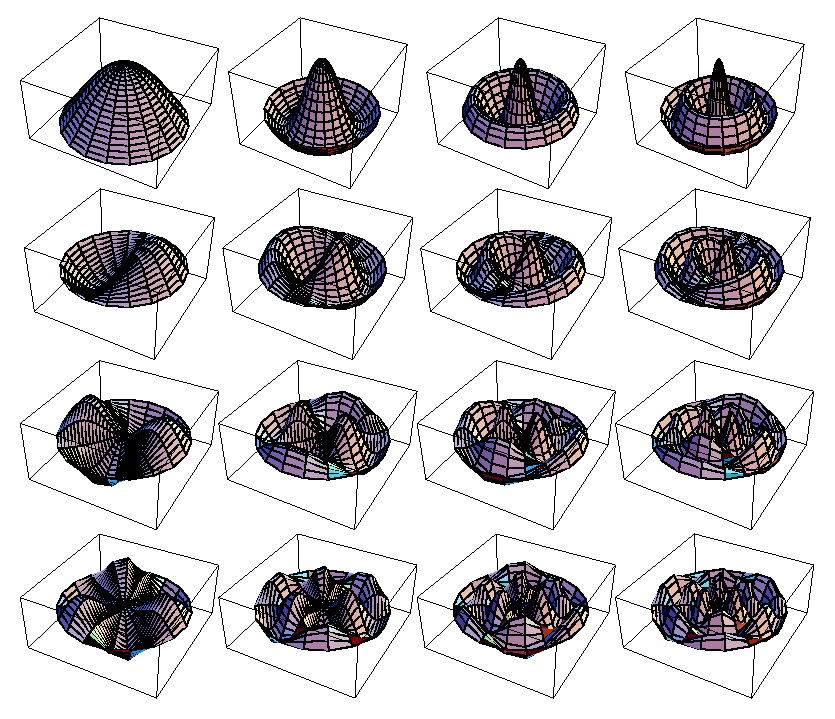
\includegraphics[width=0.95\textwidth]{pde/separation/normalmode0134}
    \end{center}
    \caption{The normal modes.}
    \label{normalmode0134}
  \end{figure}

\end{Solution}










%% Diffusion equation with zero boundary conditions
\begin{Solution}
  \label{solution diffusion equation zero bc}
  We will expand the solution in a complete, orthogonal set of functions
  $\{X_n(x)\}$, where the coefficients are functions of $t$.
  \[
  \phi = \sum_n T_n(t) X_n(x)
  \]
  We will use separation of variables to determine a convenient set $\{X_n\}$.
  We substitite $\phi = T(t) X(x)$ into the diffusion equation.
  \begin{gather*}
    \phi_t = a^2 \phi_{x x} \\
    X T' = a^2 X'' T \\
    \frac{T'}{a^2 T} = \frac{X''}{X} = - \lambda \\
    T' = -a^2 \lambda T, \quad X'' + \lambda X = 0
  \end{gather*}
  Note that in order to satisfy 
  $\phi(0,t) = \phi(l,t) = 0$, the $X_n$ must satisfy the same homogeneous
  boundary conditions, $X_n(0) = X_n(l) = 0$.  This gives us a 
  Sturm-Liouville problem for $X(x)$.
  \begin{gather*}
    X'' + \lambda X = 0, \quad X(0) = X(l) = 0 \\
    \lambda_n = \left( \frac{n \pi}{l} \right)^2, \quad
    X_n = \sin \left( \frac{n \pi x}{l} \right), \quad 
    n \in \mathbb{Z}^+
  \end{gather*}

  Thus we seek a solution of the form
  \begin{equation}
    \label{eqn_phi_sumoi_Tn_sin}
    \phi = \sum_{n=1}^\infty T_n(t) \sin \left( \frac{n \pi x}{l} \right).
  \end{equation}
  This solution automatically satisfies the boundary conditions.  We will 
  assume that we can differentiate it.  We will substitite this form into
  the diffusion equation and the initial condition to determine the 
  coefficients in the series, $T_n(t)$.
  First we substitute Equation~\ref{eqn_phi_sumoi_Tn_sin}
  into the partial differential equation for
  $\phi$ to determine ordinary differential equations for the $T_n$.
  \begin{gather*}
    \phi_t = a^2 \phi_{x x} \\
    \sum_{n=1}^\infty T_n'(t) \sin \left( \frac{n \pi x}{l} \right)
    = - a^2 \sum_{n=1}^\infty \left( \frac{n \pi}{l} \right)^2 T_n(t) 
    \sin \left( \frac{n \pi x}{l} \right) \\
    T_n' = - \left( \frac{a n \pi}{l} \right)^2 T_n \\
  \end{gather*}
  Now we substitute Equation~\ref{eqn_phi_sumoi_Tn_sin}
  into the initial condition for $\phi$ to determine 
  initial conditions for the $T_n$.
  \begin{gather*}
    \sum_{n=1}^\infty T_n(0) \sin \left( \frac{n \pi x}{l} \right) = \phi(x, 0) \\
    T_n(0) = \frac{ \int_0^l \sin\left(\frac{ n \pi x}{l}\right) \phi(x, 0) \,\dd x }
    { \int_0^l \sin^2 \left(\frac{ n \pi x}{l}\right) \,\dd x } \\
    T_n(0) = \frac{2}{l} \int_0^l \sin\left(\frac{ n \pi x}{l}\right) 
    \phi(x, 0) \,\dd x \\
    T_n(0) = \frac{2}{l} \int_0^{l/2} \sin\left(\frac{ n \pi x}{l}\right) x \,\dd x
    + \frac{2}{l} \int_0^{l/2} \sin\left(\frac{ n \pi x}{l}\right)
    (l-x) \,\dd x \\
    T_n(0) = \frac{4 l}{n^2 \pi^2} \sin \left( \frac{n \pi}{2} \right) \\
    T_{2n-1}(0) = (-1)^n \frac{4 l}{(2n-1)^2 \pi^2}, \quad
    T_{2n}(0) = 0, \quad n \in \mathbb{Z}^+
  \end{gather*}
  We solve the ordinary differential equations for $T_n$ subject to the 
  initial conditions.
  \[
  T_{2n-1}(t) = (-1)^n \frac{4 l}{(2n-1)^2 \pi^2} 
  \exp \left( - \left( \frac{a (2n-1) \pi}{l} \right)^2 t \right), \quad
  T_{2n}(t) = 0, \quad n \in \mathbb{Z}^+
  \]
  This determines the series representation of the solution.
  \[
  \boxed{
    \phi = \frac{4}{l}\sum_{n=1}^\infty (-1)^n \left( \frac{l}{(2n-1) \pi} \right)^2
    \exp \left( - \left( \frac{a (2n-1) \pi}{l} \right)^2 t \right)
    \sin \left( \frac{(2n-1) \pi x}{l} \right)
    }
  \]

  From the initial condition, we know that the
  the solution at $t = 0$ is $C^0$.  That is, it is continuous, but not 
  differentiable.  The series representation of the solution at $t = 0$ is
  \[
  \phi = \frac{4}{l}\sum_{n=1}^\infty (-1)^n \left( \frac{l}{(2n-1) \pi} \right)^2
  \sin \left( \frac{(2n-1) \pi x}{l} \right).
  \]
  That the coefficients decay as $1/n^2$ corroborates that $\phi(x,0)$ 
  is $C^0$.

  The derivatives of $\phi$ with respect to $x$ are
  \begin{gather*}
    \frac{\partial^{2m-1}}{\partial x^{2m-1}}\phi 
    = \frac{4(-1)^{m+1}}{l} \sum_{n=1}^\infty (-1)^n \left( \frac{(2n-1) \pi}{l}
    \right)^{2m-3}
    \exp \left( - \left( \frac{a (2n-1) \pi}{l} \right)^2 t \right)
    \cos \left( \frac{(2n-1) \pi x}{l} \right) \\
    \frac{\partial^{2m}}{\partial x^{2m}}\phi 
    = \frac{4 (-1)^m}{l} \sum_{n=1}^\infty (-1)^n \left( \frac{(2n-1) \pi}{l}
    \right)^{2m-2}
    \exp \left( - \left( \frac{a (2n-1) \pi}{l} \right)^2 t \right)
    \sin \left( \frac{(2n-1) \pi x}{l} \right)
  \end{gather*}
  For any fixed $t > 0$, the coefficients in the series for 
  $\frac{\partial^n}{\partial x} \phi$ decay exponentially.  These series are
  uniformly convergent in $x$.  Thus for any fixed $t > 0$, $\phi$ is 
  $C^\infty$ in $x$. 
\end{Solution}









%% Diffusion equation with nonzero boundary conditions
\begin{Solution}
  \label{solution diffusion nonzero bc}
  \begin{gather*}
    u_t = \kappa u_{x x}, \quad 0 < x < L, \quad t > 0 \\
    u(0,t) = T_0, \quad u(L,t) = T_1, \quad u(x,0) = f(x),
  \end{gather*}
  \textbf{Method 1.}
  We solve this problem with an eigenfunction expansion in $x$.  To find
  an appropriate set of eigenfunctions, we apply the separation of variables,
  $u(x,t) = X(x) T(t)$ to the partial differential equation with the 
  homogeneous boundary conditions, $u(0,t) = u(L,t) = 0$.  
  \begin{gather*}
    (X T)_t = (X T)_{x x} \\
    X T' = X'' T \\
    \frac{T'}{T} = \frac{X''}{X} = - \lambda^2
  \end{gather*}
  We have the eigenvalue problem,
  \[
  X'' + \lambda^2 X = 0, \quad X(0) = X(L) = 0,
  \]
  which has the solutions,
  \[
  \lambda_n = \frac{n \pi x}{L}, \quad 
  X_n = \sin \left( \frac{n \pi x}{L} \right), \quad n \in \mathbb{N}.
  \]
  We expand the solution of the partial differential equation in terms of 
  these eigenfunctions.
  \[
  \boxed{
    u(x,t) = \sum_{n=1}^\infty a_n(t) \sin \left( \frac{n \pi x}{L} \right)
    }
  \]
  Because of the inhomogeneous boundary conditions, the convergence of the
  series will not be uniform.  We can differentiate the series with respect to 
  $t$, but not with respect to $x$.  We multiply the partial differential
  equation by an eigenfunction and integrate from $x=0$ to $x=L$.  We
  use integration by parts to move derivatives from $u$ to the eigenfunction.
  \begin{gather*}
    u_t - \kappa u_{x x} = 0 \\
    \int_0^L \left( u_t - \kappa u_{x x} \right) \sin \left(
      \frac{m \pi x}{L} \right) \,\dd x = 0 \\
    \int_0^L \left( \sum_{n=1}^\infty a_n'(t) \sin \left( \frac{n \pi x}{L} \right) \right)
    \sin \left( \frac{m \pi x}{L} \right) \,\dd x 
    - \kappa \left[ u_x \sin \left( \frac{m \pi x}{L} \right) \right]_0^L
    + \kappa \frac{m \pi}{L} 
    \int_0^L u_x \cos \left( \frac{m \pi x}{L} \right) \,\dd x = 0 \\
    \frac{L}{2} a_m'(t) 
    + \kappa \frac{m \pi}{L} 
    \left[ u \cos \left( \frac{m \pi x}{L} \right) \right]_0^L
    + \kappa \left( \frac{m \pi}{L} \right)^2
    \int_0^L u \sin \left( \frac{m \pi x}{L} \right) \,\dd x = 0 \\
    \frac{L}{2} a_m'(t) 
    + \kappa \frac{m \pi}{L} \left( (-1)^m u(L,t) - u(0,t) \right)
    + \kappa \left( \frac{m \pi}{L} \right)^2
    \int_0^L \left( \sum_{n=1}^\infty a_n(t) \sin \left( \frac{n \pi x}{L} \right)
    \right) \sin \left( \frac{m \pi x}{L} \right) \,\dd x = 0 \\
    \frac{L}{2} a_m'(t) 
    + \kappa \frac{m \pi}{L} \left( (-1)^m T_1 - T_0 \right)
    + \kappa \frac{L}{2} \left( \frac{m \pi}{L} \right)^2 a_m(t) = 0 \\
    a_m'(t) + \kappa \left( \frac{m \pi}{L} \right)^2 a_m(t) 
    = \kappa \frac{2 m \pi}{L^2} \left( T_0 - (-1)^m T_1 \right)
  \end{gather*}
  Now we have a first order differential equation for each of the $a_n$'s.
  We obtain initial conditions for each of the $a_n$'s from the initial 
  condition for $u(x,t)$.
  \begin{gather*}
    u(x,0) = f(x) \\
    \sum_{n=1}^\infty a_n(0) \sin \left( \frac{n \pi x}{L} \right) = f(x) \\
    a_n(0) = \frac{2}{L} \int_0^L f(x) \sin \left( \frac{n \pi x}{L} \right)\,\dd x
    \equiv f_n
  \end{gather*}
  By solving the first order differential equation for $a_n(t)$, we obtain
  \[
  \boxed{
    a_n(t) = \frac{ 2 (T_0 - (-1)^n T_1) }{ n \pi }
    + \e^{- \kappa (n \pi / L)^2 t } \left( f_n - 
      \frac{ 2 (T_0 - (-1)^n T_1) }{ n \pi } \right).
    }
  \]
  Note that the series does not converge uniformly due to the $1/n$ term.




  \textbf{Method 2.}
  For our second method we transform the problem to one with homogeneous
  boundary conditions so that we can use the partial differential equation
  to determine the time dependence of the eigen-solutions.
  We make the change of variables $v(x,t) = u(x,t) - \mu(x)$
  where $\mu(x)$ is some function that satisfies the inhomogeneous boundary
  conditions.   If possible, we want $\mu(x)$ to satisfy the partial differential
  equation as well.  For this problem we can choose $\mu(x)$ to be the 
  equilibrium solution which satisfies
  \[
  \mu''(x) = 0, \quad \mu(0) T_0, \quad \mu(L) = T_1.
  \]
  This has the solution
  \[
  \mu(x) = T_0 + \frac{T_1-T_0}{L} x.
  \]
  With the change of variables,
  \[
  v(x,t) = u(x,t) - \left( T_0 + \frac{T_1-T_0}{L} x \right),
  \]
  we obtain the problem
  \begin{gather*}
    v_t = \kappa v_{x x}, \quad 0 < x < L, \quad t > 0 \\
    v(0,t) = 0, \quad v(L,t) = 0, \quad 
    v(x,0) = f(x) - \left( T_0 + \frac{T_1-T_0}{L} x \right).
  \end{gather*}
  Now we substitute the separation of variables $v(x,t) = X(x) T(t)$ into 
  the partial differential equation.
  \begin{gather*}
    (X T)_t = \kappa (X T)_{x x} \\
    \frac{T'}{\kappa T} = \frac{X''}{X} = -\lambda^2
  \end{gather*}
  Utilizing the boundary conditions at $x = 0,L$ we obtain the two ordinary
  differential equations,
  \begin{gather*}
    T' = - \kappa \lambda^2 T, \\
    X'' = - \lambda^2 X, \quad X(0) = X(L) = 0.
  \end{gather*}
  The problem for $X$ is a regular Sturm-Liouville problem and has the solutions
  \[
  \lambda_n = \frac{n\pi}{L}, \quad
  X_n = \sin \left( \frac{n \pi x}{L} \right), \quad n \in \mathbb{N}.
  \]
  The ordinary differential equation for $T$ becomes,
  \[
  T_n' = - \kappa \left( \frac{ n \pi }{L} \right)^2 T_n,
  \]
  which, (up to a multiplicative constant), has the solution,
  \[
  T_n = \e^{- \kappa (n \pi / L)^2 t}.
  \]
  Thus the eigenvalues and eigen-solutions of the partial differential 
  equation are,
  \[
  \lambda_n = \frac{n\pi}{L}, \quad
  v_n = \sin \left( \frac{n \pi x}{L} \right) \e^{-\kappa (n\pi/L)^2 t}, \quad 
  n \in \mathbb{N}.
  \]
  Let $v(x,t)$ have the series expansion,
  \[
  v(x,t) = \sum_{n=1}^\infty a_n \sin \left( \frac{n \pi x}{L} \right) 
  \e^{-\kappa (n\pi/L)^2 t}.
  \]
  We determine the coefficients in the expansion from the initial condition,
  \[
  v(x,0) = \sum_{n=1}^\infty a_n \sin \left( \frac{n \pi x}{L} \right) 
  = f(x) - \left( T_0 + \frac{T_1 - T_0}{L} x \right).
  \]
  The coefficients in the expansion are the Fourier sine coefficients of
  $f(x) - \left( T_0 + \frac{T_1 - T_0}{L} x \right)$.
  \begin{gather*}
    a_n = \frac{2}{L} \int_0^L \left( 
      f(x) - \left( T_0 + \frac{T_1 - T_0}{L} x \right) \right)
    \sin \left( \frac{n \pi x}{L} \right) \,\dd x \\
    a_n = f_n - \frac{ 2 (T_0 - (-1)^n T_1) }{ n \pi } 
  \end{gather*}
  With the coefficients defined above, the solution for $u(x,t)$ is
  \[
  \boxed{
    u(x,t) = T_0 + \frac{T_1 - T_0}{L} x 
    + \sum_{n=1}^\infty \left( f_n - \frac{ 2 (T_0 - (-1)^n T_1) }{ n \pi } \right)
    \sin \left( \frac{n \pi x}{L} \right) \e^{-\kappa (n\pi/L)^2 t}.
    }
  \]
  Since the coefficients in the sum decay exponentially for $t>0$, we 
  see that the series is uniformly convergent for positive $t$.
  It is clear that the two solutions we have obtained are equivalent.
\end{Solution}







%% \phi_t = a^2 \phi_{xx} + w(x,t), \phi(0,t) = 0,\quad \phi_x(l,t) = 0
\begin{Solution}
  \label{solution pt=a2pxx+w p=0 px=0}
  First we solve the eigenvalue problem for $\beta(x)$, which is the
  problem we would obtain if we applied separation of variables to the
  partial differential equation, $\phi_t = \phi_{x x}$.  We have the
  eigenvalues and orthonormal eigenfunctions
  \[
  \lambda_n = \left( \frac{ (2n-1) \pi }{ 2 l } \right)^2, \quad
  \beta_n(x) = \sqrt{ \frac{2}{l} } \sin \left( \frac{ (2n-1) \pi x }
    { 2 l } \right), \quad
  n \in \mathbb{Z}^+.
  \]
  We expand the solution and inhomogeneity in Equation
  ~\ref{phi_t=a2phi_xx+w} in a series of the eigenvalues.
  \begin{gather*}
    \phi(x,t) = \sum_{n=1}^\infty T_n(t) \beta_n(x) \\
    w(x,t) = \sum_{n=1}^\infty w_n(t) \beta_n(x), \quad
    w_n(t) = \int_0^l \beta_n(x) w(x,t) \,\dd x
  \end{gather*}
  Since $\phi$ satisfies the same homgeneous boundary conditions as
  $\beta$, we substitute the series into Equation~\ref{phi_t=a2phi_xx+w}
  to determine differential equations for the $T_n(t)$.
  \begin{gather*}
    \sum_{n=1}^\infty T_n'(t) \beta_n(x) 
    = a^2 \sum_{n=1}^\infty T_n(t) (-\lambda_n) \beta_n(x)
    + \sum_{n=1}^\infty w_n(t) \beta_n(x) \\
    T_n'(t) = - a^2 \left( \frac{ (2n-1) \pi }{ 2 l } \right)^2 T_n(t)
    + w_n(t)
  \end{gather*}
  Now we substitute the series for $\phi$ into its initial condition to
  determine initial conditions for the $T_n$.
  \begin{gather*}
    \phi(x,0) = \sum_{n=1}^\infty T_n(0) \beta_n(x) = f(x) \\
    T_n(0) = \int_0^l \beta_n(x) f(x) \,\dd x
  \end{gather*}
  We solve for $T_n(t)$ to determine the solution, $\phi(x,t)$.
  \[
  T_n(t) = \exp \left( - \left( \frac{ (2n-1) a \pi }{ 2 l } \right)^2
    t \right) \left( T_n(0) + \int_0^t w_n(\tau) 
    \exp \left( \left( \frac{ (2n-1) a \pi }{ 2 l } \right)^2
      \tau \right) \,\dd \tau \right)
  \]
\end{Solution}





%% Heat equation, \phi(0,t) = 0, \quad c \phi(l,t) + \phi_x(l,t) = 0.
\begin{Solution}
  \label{solution heat p=0 cp+px=0}
  Separation of variables leads to the eigenvalue problem
  \[
  \beta'' + \lambda \beta = 0, \quad
  \beta(0) = 0, \quad
  \beta(l) + c \beta'(l) = 0.
  \]
  First we consider the case $\lambda = 0$.  A set of solutions of the
  differential equation is $\{ 1, x \}$.  The solution that satisfies
  the left boundary condition is $\beta(x) = x$.  The right boundary
  condition imposes the constraint $l + c = 0$.  Since $c$ is positive,
  this has no solutions.  $\lambda = 0$ is not an eigenvalue.

  Now we consider $\lambda \neq 0$.  A set of solutions of the
  differential equation is $\{\cos(\sqrt{\lambda} x),
  \sin(\sqrt{\lambda} x) \}$.  The solution that satisfies the left
  boundary condition is $\beta = \sin(\sqrt{\lambda} x)$.  The right
  boundary condition imposes the constraint
  \begin{gather*}
    c \sin \left( \sqrt{\lambda} l \right) + \sqrt{\lambda} 
    \cos \left( \sqrt{\lambda} l \right) = 0 \\
    \tan \left( \sqrt{\lambda} l \right) = - \frac{ \sqrt{\lambda} }{c}
  \end{gather*}
  For large $\lambda$, the we can determine approximate solutions.
  \begin{gather*}
    \sqrt{ \lambda_n } l \approx \frac{ (2n-1) \pi }{ 2 },
    n \in \mathbb{Z}^+ \\
    \lambda_n \approx \left( \frac{ (2n-1) \pi }{ 2 l } \right)^2,
    n \in \mathbb{Z}^+
  \end{gather*}
  The eigenfunctions are
  \[
  \beta_n(x) = \frac{ \sin \left( \sqrt{ \lambda_n } x \right) }
  { \sqrt{ \int_0^l \sin^2 \left( \sqrt{ \lambda_n } x 
      \right) \,\dd x } }, n \in \mathbb{Z}^+.
  \]

  We expand $\phi(x,t)$ and $w(x,t)$ in series of the eigenfunctions.
  \begin{gather*}
    \phi(x,t) = \sum_{n=1}^\infty T_n(t) \beta_n(x) \\
    w(x,t) = \sum_{n=1}^\infty w_n(t) \beta_n(x), \quad
    w_n(t) = \int_0^l \beta_n(x) w(x,t) \,\dd x
  \end{gather*}
  Since $\phi$ satisfies the same homgeneous boundary conditions as
  $\beta$, we substitute the series into Equation~\ref{phi_t=a2phi_xx+w}
  to determine differential equations for the $T_n(t)$.
  \begin{gather*}
    \sum_{n=1}^\infty T_n'(t) \beta_n(x) 
    = a^2 \sum_{n=1}^\infty T_n(t) (-\lambda_n) \beta_n(x)
    + \sum_{n=1}^\infty w_n(t) \beta_n(x) \\
    T_n'(t) = - a^2 \lambda_n T_n(t) + w_n(t)
  \end{gather*}
  Now we substitute the series for $\phi$ into its initial condition to
  determine initial conditions for the $T_n$.
  \begin{gather*}
    \phi(x,0) = \sum_{n=1}^\infty T_n(0) \beta_n(x) = f(x) \\
    T_n(0) = \int_0^l \beta_n(x) f(x) \,\dd x
  \end{gather*}
  We solve for $T_n(t)$ to determine the solution, $\phi(x,t)$.
  \[
  T_n(t) = \exp \left( - a^2 \lambda_n t \right) 
  \left( T_n(0) + \int_0^t w_n(\tau) 
    \exp \left( a^2 \lambda_n \tau \right) \,\dd \tau \right)
  \]
\end{Solution}





%% Heat equation, \phi(0,t) = t, \quad \phi_x(l,t) = - c\phi(l,t)
\begin{Solution}
  \label{solution heat p=t px=-cp}
  First we seek a function $u(x,t)$ that satisfies the boundary conditions
  $u(0,t) = t$, $u_x(l,t) = -c u(l,t)$.  We try a function of the form
  $u = (a x + b) t$.  The left boundary condition imposes the constraint
  $b = 1$.  We then apply the right boundary condition no determine $u$.
  \begin{gather*}
    a t = -c (a l + 1) t \\
    a = - \frac{ c }{ 1 + c l } \\
    u(x,t) = \left( 1 - \frac{ c x }{ 1 + c l } \right) t
  \end{gather*}

  Now we define $\psi$ to be the difference of $\phi$ and $u$.
  \[
  \psi(x,t) = \phi(x,t) - u(x,t)
  \]
  $\psi$ satisfies an inhomogeneous diffusion equation with homogeneous
  boundary conditions.
  \begin{gather*}
    (\psi + u)_t = a^2 (\psi + u)_{x x} + 1 \\
    \psi_t = a^2 \psi_{x x} + 1 + a^2 u_{x x} - u_t \\
    \psi_t = a^2 \psi_{x x} + \frac{ c x }{ 1 + c l }
  \end{gather*}
  The initial and boundary conditions for $\psi$ are
  \[
  \psi(x, 0) = 0, \quad
  \psi(0, t) = 0, \quad
  \psi_x(l,t) = - c \psi(l,t).
  \]
  We solved this system in problem 2.  Just take
  \[
  w(x,t) = \frac{ c x }{ 1 + c l }, \quad
  f(x) = 0.
  \]
  The solution is
  \begin{gather*}
    \psi(x,t) = \sum_{n=1}^\infty T_n(t) \beta_n(x), \\
    T_n(t) = \int_0^t w_n
    \exp \left( - a^2 \lambda_n (t - \tau) \right) \,\dd \tau, \\
    w_n(t) = \int_0^l \beta_n(x) \frac{ c x }{ 1 + c l } \,\dd x.
  \end{gather*}
  This determines the solution for $\phi$.
\end{Solution}





%% Heat eqn.  Radiation BC.  2 series solutions.
\begin{Solution}
  \label{solution heat radiation bc 2 series solutions}
  First we solve this problem with a series expansion.  We transform the
  problem to one with homogeneous boundary conditions.  Note that
  \[
  u(x) = \frac{ x }{l + 1}
  \] 
  satisfies the boundary conditions.  (It is the equilibrium solution.)
  We make the change of variables
  $\psi = \phi - u$.   The problem for $\psi$ is
  \begin{gather*}
    \psi_t = a^2 \psi_{xx}, \\
    \psi(0,t) = \psi(l,t) + \psi_x(l,t) = 0, \quad \psi(x,0) = \frac{ x }{l + 1}.
  \end{gather*}
  This is a particular case of what we solved in 
  Exercise~\ref{Heat_equation,phi(0,t)=0,quadcphi(l,t)+phi_x(l,t)=0}.
  We apply the result of that problem.  The solution for $\phi(x,t)$ is
  \begin{gather*}
    \phi(x,t) = \frac{ x }{l + 1} + \sum_{n=1}^\infty T_n(t) \beta_n(x) \\
    \beta_n(x) = \frac{ \sin \left( \sqrt{\lambda_n} x \right) }
    { \sqrt{ \int_0^l \sin^2 \left( \sqrt{ \lambda_n } x 
        \right) \,\dd x } }, \quad n \in \mathbb{Z}^+ \\
    \tan \left( \sqrt{\lambda} l \right) = - \sqrt{\lambda} \\
    T_n(t) = T_n(0) \exp \left( - a^2 \lambda_n t \right) \\
    T_n(0) = \int_0^l \beta_n(x) \frac{ x }{l + 1} \,\dd x
  \end{gather*}
  This expansion is useful for large $t$ because the coefficients decay
  exponentially with increasing $t$.

  Now we solve this problem with the Laplace transform.
  \begin{gather*}
    \phi_t = a^2\phi_{xx}, \quad \phi(0,t) = 0, \quad 
    \phi(l,t) + \phi_x(l,t) = 1, \quad \phi(x,0) = 0 \\
    s \hat{\phi} = a^2 \hat{\phi}_{x x}, \quad
    \hat{\phi}(0,s) = 0, \quad 
    \hat{\phi}(l,s) + \hat{\phi}_x(l,s) = \frac{1}{s} \\
    \hat{\phi}_{x x} - \frac{s}{a^2} \hat{\phi} = 0, \quad
    \hat{\phi}(0,s) = 0, \quad 
    \hat{\phi}(l,s) + \hat{\phi}_x(l,s) = \frac{1}{s} \\
    \intertext{The solution that satisfies the left boundary condition is}
    \hat{\phi} = c \sinh \left( \frac{ \sqrt{s} x }{ a } \right). \\
    \intertext{We apply the right boundary condition to determine the
      constant.}
    \hat{\phi} = \frac{ \sinh \left( \frac{ \sqrt{s} x }{ a } \right) }
    { s \left( \sinh \left( \frac{ \sqrt{s} l }{ a } \right)
        + \frac{ \sqrt{s} }{ a }
        \cosh \left( \frac{ \sqrt{s} l }{ a } \right) \right) } \\
    \intertext{We expand this in a series of simpler functions of $s$.}
    \hat{\phi} = \frac{ 2 \sinh \left( \frac{ \sqrt{s} x }{ a } \right) }
    { s \left( \exp \left( \frac{ \sqrt{s} l }{ a } \right)
        - \exp \left( - \frac{ \sqrt{s} l }{ a } \right)
        + \frac{ \sqrt{s} }{ a } \left(
          \exp \left( \frac{ \sqrt{s} l }{ a } \right)
          + \exp \left( - \frac{ \sqrt{s} l }{ a } \right)
        \right) \right) } \\
    \hat{\phi} = \frac{ 2 \sinh \left( \frac{ \sqrt{s} x }{ a } \right) }
    { s \exp \left( \frac{ \sqrt{s} l }{ a } \right) } \ 
    \frac{ 1 }{ 1 + \frac{ \sqrt{s} }{ a }
      - \left( 1 - \frac{ \sqrt{s} }{ a } \right)
      \exp \left( - \frac{ 2 \sqrt{s} l }{ a } \right) } \\
    \hat{\phi} = \frac{ \exp \left( \frac{ \sqrt{s} x }{ a } \right)
      - \exp \left( - \frac{ \sqrt{s} x }{ a } \right) }
    { s \left( 1 + \frac{ \sqrt{s} }{ a } \right) 
      \exp \left( \frac{ \sqrt{s} l }{ a } \right) } \ 
    \frac{ 1 }{ 1 
      - \left( \frac{ 1 - \sqrt{s} / a }{ 1 + \sqrt{s} / a } \right)
      \exp \left( - \frac{ 2 \sqrt{s} l }{ a } \right) } \\
    \hat{\phi} = \frac{ \exp \left( \frac{ \sqrt{s} (x-l) }{ a } \right)
      - \exp \left( \frac{ \sqrt{s} (-x-l) }{ a } \right) }
    { s \left( 1 + \frac{ \sqrt{s} }{ a } \right) } 
    \sum_{n=0}^\infty \left( \frac{ 1 - \sqrt{s} / a }
      { 1 + \sqrt{s} / a } \right)^n
    \exp \left( - \frac{ 2 \sqrt{s} l n }{ a } \right)
  \end{gather*}
  \begin{multline*}
    \hat{\phi} = \frac{ 1 }{ s } 
    \Bigg(
    \sum_{n=0}^\infty \frac{ (1 - \sqrt{s} / a)^n }
    { (1 + \sqrt{s} / a)^{n+1} }
    \exp \left( - \frac{ \sqrt{s} ((2n+1)l-x) }{ a } \right) \\
    - \sum_{n=0}^\infty \frac{ (1 - \sqrt{s} / a)^n }
    { (1 + \sqrt{s} / a)^{n+1} }
    \exp \left( - \frac{ \sqrt{s} ((2n+1)l+x) }{ a } \right) 
    \Bigg) 
  \end{multline*}
  By expanding 
  \[
  \frac{ (1 - \sqrt{s} / a)^n }{ (1 + \sqrt{s} / a)^{n+1} }
  \]
  in binomial series all the terms would be of the form
  \[
  s^{-m/2-3/2} \exp \left( - \frac{ \sqrt{s} ((2n \pm 1)l \mp x) }{ a } \right).
  \]
  Taking the first term in each series yields
  \[
  \hat{\phi} \sim \frac{ a }{ s^{3/2} } \left(
    \exp \left( - \frac{ \sqrt{s} (l-x) }{ a } \right)
    - \exp \left( - \frac{ \sqrt{s} (l+x) }{ a } \right) \right),
  \quad \mathrm{as}\ s \to \infty.
  \]
  We take the inverse Laplace transform to obtain an appoximation of
  the solution for $t \ll 1$.
  \begin{multline*}
    \phi(x,t) \sim 2 a^2 \sqrt{\pi t} \left(
      \frac{ \exp \left( - \frac{ (l-x)^2 }{ 4 a^2 t } \right) }{ l - x }
      -\frac{ \exp \left( - \frac{ (l+x)^2 }{ 4 a^2 t } \right) }{ l + x }
    \right) \\ 
    - \pi \left( \erfc \left( \frac{ l - x }{ 2 a \sqrt{t} } \right)
      - \erfc \left( \frac{ l + x }{ 2 a \sqrt{t} } \right) \right),
    \quad \mathrm{for}\ t \ll 1
  \end{multline*}
\end{Solution}






%% \phi_t = A^2(x^2 \phi_x)_x, where $A$ is a  constant. 
\begin{Solution}
  \label{solution pt=A2x2pxx}
  We apply the separation of variables $\phi(x,t) = X(x) T(t)$.
  \begin{gather*}
    \phi_t = A^2 \left( x^2 \phi_x \right)_x 
    \\
    X T' = T A^2 \left( x^2 X' \right)' 
    \\
    \frac{ T' }{ A^2 T } = \frac{ (x^2 X')' }{ X } = - \lambda
  \end{gather*}
  This gives us a regular Sturm-Liouville problem.
  \[
  \left( x^2 X' \right)' + \lambda X = 0, \quad
  X(1) = X(2) = 0
  \]
  This is an Euler equation.  We make the substitution $X = x^\alpha$ to find the 
  solutions.
  \begin{gather}
    \label{x2X+2xX+lambdaX=0}
    x^2 X'' + 2 x X' + \lambda X = 0 
    \\
    \nonumber
    \alpha ( \alpha - 1 ) + 2 \alpha + \lambda = 0 
    \\
    \nonumber
    \alpha = \frac{ -1 \pm \sqrt{ 1 - 4 \lambda } }{ 2 } 
    \\
    \nonumber
    \alpha = - \frac{1}{2} \pm \imath \sqrt{ \lambda - 1/4 }
  \end{gather}

  First we consider the case of a double root when $\lambda = 1/4$.
  The solutions of Equation~\ref{x2X+2xX+lambdaX=0} are 
  $\{ x^{-1/2}, x^{-1/2} \ln x \}$.  The solution that satisfies the
  left boundary condition is $X = x^{-1/2} \ln x$.  Since this does not
  satisfy the right boundary condition, $\lambda = 1/4$ is not an
  eigenvalue.

  Now we consider $\lambda \neq 1/4$.  
  The solutions of Equation~\ref{x2X+2xX+lambdaX=0} are 
  \[
  \left\{ 
    \frac{ 1 }{ \sqrt{x} } \cos \left( \sqrt{ \lambda - 1/4 } \ln x \right), 
    \frac{ 1 }{ \sqrt{x} } \sin \left( \sqrt{ \lambda - 1/4 } \ln x \right) 
  \right\}.
  \]
  The solution that satisfies the left boundary condition is
  \[
  \frac{ 1 }{ \sqrt{x} } \sin \left( \sqrt{ \lambda - 1/4 } \ln x \right).
  \]
  The right boundary condition imposes the constraint
  \[
  \sqrt{ \lambda - 1/4 } \ln 2 = n \pi, \quad n \in \mathbb{Z}^+.
  \]
  This gives us the eigenvalues and eigenfunctions.
  \[
  \lambda_n = \frac{1}{4} + \left( \frac{ n \pi }{ \ln 2 } \right)^2,
  \quad
  X_n(x) = \frac{ 1 }{ \sqrt{x} } \sin \left( 
    \frac{ n \pi \ln x }{ \ln 2 } \right),
  \quad n \in \mathbb{Z}^+.
  \]
  We normalize the eigenfunctions.
  \begin{gather*}
    \int_1^2 \frac{1}{x} \sin^2 \left( 
      \frac{ n \pi \ln x }{ \ln 2 } \right) \,\dd x
    = \ln 2 \int_0^1 \sin^2 ( n \pi \xi ) \,\dd \xi
    = \frac{ \ln 2 }{ 2 } 
    \\
    X_n(x) = \sqrt{ \frac{ 2 }{ \ln 2 } }
    \frac{ 1 }{ \sqrt{x} } \sin \left( 
      \frac{ n \pi \ln x }{ \ln 2 } \right),
    \quad n \in \mathbb{Z}^+.
  \end{gather*}

  From separation of variables, we have differential equations for the $T_n$.
  \begin{gather*}
    T_n' = - A^2 \left( \frac{1}{4} + \left( \frac{ n \pi }{ \ln 2 } \right)^2
    \right) T_n
    \\
    T_n(t) = \exp \left( - A^2 \left( \frac{1}{4} 
        + \left( \frac{ n \pi }{ \ln 2 } \right)^2 \right) t \right)
  \end{gather*}
  We expand $\phi$ in a series of the eigensolutions.
  \[
  \phi(x,t) = \sum_{n=1}^\infty \phi_n X_n(x) T_n(t)
  \]
  We substitute the expansion for $\phi$ into the initial condition to
  determine the coefficients.
  \begin{gather*}
    \phi(x,0) = \sum_{n=1}^\infty \phi_n X_n(x) = f(x) 
    \\
    \phi_n = \int_1^2 X_n(x) f(x) \,\dd x
  \end{gather*}
\end{Solution}









%% Wave equation with fixed and free end, zero initial velocity.
\begin{Solution}
  \label{solution wave fixed free end zero}
  \begin{gather*}
    u_{t t} = c^2 u_{x x}, \quad 0 < x < L, \quad t > 0, \\
    u(0,t) = 0, \quad u_x(L,t) = 0, \\
    u(x,0) = f(x), \quad u_t(x,0) = 0,
  \end{gather*}
  We substitute the separation of variables $u(x,t) = X(x) T(t)$ into the
  partial differential equation.
  \begin{gather*}
    (X T)_{t t} = c^2 (X T)_{x x} \\
    \frac{T''}{c^2 T} = \frac{X''}{X} = -\lambda^2
  \end{gather*}
  With the boundary conditions at $x = 0, L$, we have the ordinary differential
  equations,
  \begin{gather*}
    T'' = - c^2 \lambda^2 T, \\
    X'' = - \lambda^2 X, \quad X(0) = X'(L) = 0.
  \end{gather*}
  The problem for $X$ is a regular Sturm-Liouville eigenvalue problem.  
  From the Rayleigh quotient,
  \[
  \lambda^2 = \frac{ - \left[ \phi \phi' \right]_0^L + \int_0^L (\phi')^2 \,\dd x}
  { \int_0^L \phi^2 \,\dd x }
  = \frac{ \int_0^L (\phi')^2 \,\dd x}{ \int_0^L \phi^2 \,\dd x }
  \]
  we see that there are only positive eigenvalues.
  For $\lambda^2 > 0$ the general solution of the ordinary differential 
  equation is
  \[
  X = a_1 \cos( \lambda x) + a_2 \sin( \lambda x ).
  \]
  The solution that satisfies the left boundary condition is
  \[
  X = a \sin( \lambda x ).
  \]
  For non-trivial solutions, the right boundary condition imposes the 
  constraint,
  \[
  \cos \left( \lambda L \right) = 0,
  \]
  \[
  \lambda = \frac{\pi}{L} \left( n - \frac{1}{2} \right), \quad
  n \in \mathbb{N}.
  \]
  The eigenvalues and eigenfunctions are
  \[
  \lambda_n = \frac{ (2n-1) \pi }{ 2 L }, \quad
  X_n = \sin \left( \frac{ (2n-1) \pi x }{ 2 L } \right),
  \quad n \in \mathbb{N}.
  \]
  The differential equation for $T$ becomes
  \[
  T'' = - c^2 \left( \frac{ (2n-1) \pi }{ 2 L } \right)^2 T,
  \]
  which has the two linearly independent solutions,
  \[
  T_n^{(1)} = \cos \left( \frac{ (2n-1) c \pi t }{ 2 L } \right), \quad
  T_n^{(2)} = \sin \left( \frac{ (2n-1) c \pi t }{ 2 L } \right).
  \]
  The eigenvalues and eigen-solutions of the partial differential equation are,
  \[
  \lambda_n = \frac{ (2n-1) \pi }{ 2 L }, \quad n \in \mathbb{N},
  \]
  \[
  u_n^{(1)} = \sin \left( \frac{ (2n-1) \pi x }{ 2 L } \right)
  \cos \left( \frac{ (2n-1) c \pi t }{ 2 L } \right), \quad
  u_n^{(2)} = \sin \left( \frac{ (2n-1) \pi x }{ 2 L } \right)
  \sin \left( \frac{ (2n-1) c \pi t }{ 2 L } \right).
  \]
  We expand $u(x,t)$ in a series of the eigen-solutions.
  \[
  u(x,t) = \sum_{n=1}^\infty \sin \left( \frac{ (2n-1) \pi x }{ 2 L } \right)
  \left( a_n \cos \left( \frac{ (2n-1) c \pi t }{ 2 L } \right)
    + b_n \sin \left( \frac{ (2n-1) c \pi t }{ 2 L } \right) \right).
  \]
  We impose the initial condition $u_t(x,0) = 0$,
  \[
  u_t(x,0) = \sum_{n=1}^\infty b_n \frac{ (2n-1) c \pi }{ 2 L } 
  \sin \left( \frac{ (2n-1) \pi x }{ 2 L } \right) = 0,
  \]
  \[
  b_n = 0.
  \]
  The initial condition $u(x,0) = f(x)$ allows us to determine the remaining
  coefficients,
  \[
  u(x,0) = \sum_{n=1}^\infty a_n \sin \left( \frac{ (2n-1) \pi x }{ 2 L } \right) = f(x),
  \]
  \[
  \boxed{
    a_n = \frac{2}{L} \int_0^L f(x) 
    \sin \left( \frac{ (2n-1) \pi x }{ 2 L } \right)\,\dd x.
    }
  \]
  The series solution for $u(x,t)$ is, 
  \[
  \boxed{
    u(x,t) = \sum_{n=1}^\infty a_n \sin \left( \frac{ (2n-1) \pi x }{ 2 L } \right)
    \cos \left( \frac{ (2n-1) c \pi t }{ 2 L } \right).
    }
  \]
\end{Solution}




%% Potential equation
\begin{Solution}
  \label{solution potential 2d block zero insulated}
  \begin{gather*}
    u_{x x} + u_{y y} = f(x, y), \quad 0 < x < a, \quad 0 < y < b, 
    \\
    u(0,y) = u(a,y) = 0, \quad u_y(x,0) = u_y(x,b) = 0
  \end{gather*}
  We will solve this problem with an eigenfunction expansion in $x$.  
  To determine a suitable set of eigenfunctions, 
  we substitute the separation of variables $u(x,y) = X(x) Y(y)$ into the
  homogeneous partial differential equation.
  \begin{gather*}
    u_{x x} + u_{y y} = 0 
    \\
    (X Y)_{x x} + (X Y)_{y y} = 0 
    \\
    \frac{X''}{X} = - \frac{Y''}{Y} = - \lambda^2
  \end{gather*}
  With the boundary conditions at $x = 0,a$, we have the regular 
  Sturm-Liouville problem,
  \[
  X'' = -\lambda^2 X, \quad X(0) = X(a) = 0,
  \]
  which has the solutions,
  \[
  \lambda_n = \frac{n \pi}{a}, \quad
  X_n = \sin \left( \frac{n \pi x}{a} \right), \quad
  n \in \mathbb{Z}^+.
  \]
  We expand $u(x,y)$ in a series of the eigenfunctions.
  \[
  \boxed{
    u(x,y) = \sum_{n=1}^\infty u_n(y) \sin \left( \frac{n \pi x}{a} \right)
    }
  \]
  We substitute this series into the partial differential equation and boundary
  conditions at $y = 0, b$.
  \begin{gather*}
    \sum_{n=1}^\infty \left( - \left( \frac{n \pi}{a} \right)^2 
      u_n(y) \sin \left( \frac{n \pi x}{a} \right)
      + u_n''(y) \sin \left( \frac{n \pi x}{a} \right) \right) = f(x)
    \\
    \sum_{n=1}^\infty u_n'(0) \sin \left( \frac{n \pi x}{a} \right) =
    \sum_{n=1}^\infty u_n'(b) \sin \left( \frac{n \pi x}{a} \right) = 0
  \end{gather*}
  We expand $f(x,y)$ in a Fourier sine series.
  \begin{gather*}
    f(x,y) = \sum_{n=1}^\infty f_n(y) \sin \left( \frac{n \pi x}{a} \right)
    \\
    \boxed{
      f_n(y) = \frac{2}{a} \int_0^a f(x,y) \sin \left( \frac{n \pi x}{a} \right) \,\dd x
      }
  \end{gather*}
  We obtain the ordinary differential equations for the coefficients in the 
  expansion.
  \[
  u_n''(y) - \left( \frac{n \pi}{a} \right)^2 u_n(y) = f_n(y), \quad
  u_n'(0) = u_n'(b) = 0, \quad n \in \mathbb{Z}^+.
  \]
  We will solve these ordinary differential equations with Green functions.

  Consider the Green function problem,
  \[
  g_n''(y;\eta) - \left( \frac{n \pi}{a} \right)^2 g_n(y;\eta) = \delta(y-\eta),
  \quad 
  g_n'(0;\eta) = g_n'(b;\eta) = 0.
  \]
  The homogeneous solutions
  \[
  \cosh \left( \frac{ n \pi y}{a} \right) \quad \mathrm{and} \quad
  \cosh \left( \frac{ n \pi (y-b)}{a} \right)
  \]
  satisfy the left and right boundary conditions, respectively.
  We compute the Wronskian of these two solutions.
  \begin{align*}
    W(y)    
    &= \begin{vmatrix}
      \cosh( n \pi y / a) & \cosh( n \pi (y-b) / a ) \\
      \frac{n \pi}{a} \sinh( n \pi y / a) & \frac{n \pi}{a} \sinh( n \pi (y-b) / a ) 
    \end{vmatrix} 
    \\
    &= \frac{n \pi}{a} \left( 
      \cosh \left( \frac{n \pi y}{a} \right)
      \sinh \left( \frac{n \pi (y-b)}{a} \right)
      - \sinh \left( \frac{n \pi y}{a} \right)
      \cosh \left( \frac{n \pi (y-b)}{a} \right) \right) 
    \\
    &= - \frac{n \pi}{a} \sinh \left( \frac{n \pi b}{a} \right)
  \end{align*}
  The Green function is
  \[
  \boxed{
    g_n(y;\eta) = - \frac{ a \cosh( n \pi y_< / a) \cosh( n \pi (y_>-b) / a) }
    { n \pi \sinh( n \pi b / a ) }.
    }
  \]
  The solutions for the coefficients in the expansion are
  \[
  \boxed{
    u_n(y) = \int_0^b g_n(y;\eta) f_n(\eta) \,\dd \eta.
    }
  \]
\end{Solution}












%% Vibrations of a beam.
\begin{Solution}
  \label{solution vibrations of a beam}
  \begin{gather*}
    u_{t t} + a^2 u_{x x x x} = 0, \quad 0 < x < L, t > 0, \\
    u(x,0) = f(x), \quad u_t(x,0) = g(x), \\
    u(0,t) = u_{x x}(0,t) = 0, \quad u(L,t) = u_{x x}(L,t) = 0, 
  \end{gather*}
  We will solve this problem by expanding the solution in a series of 
  eigen-solutions that satisfy the partial differential equation and the 
  homogeneous boundary conditions.  We will use the initial conditions
  to determine the coefficients in the expansion.
  We substitute the separation of variables, $u(x,t) = X(x) T(t)$ into the
  partial differential equation.
  \begin{gather*}
    (X T)_{t t} + a^2 (X T)_{x x x x} = 0 \\
    \frac{T''}{a^2 T} = - \frac{X''''}{X} = - \lambda^4
  \end{gather*}
  Here we make the assumption that $0 \leq \arg(\lambda) < \pi/2$, i.e.,
  $\lambda$ lies in the first quadrant of the complex plane.  Note that
  $\lambda^4$ covers the entire complex plane.
  We have the ordinary differential equation,
  \[
  T'' = - a^2 \lambda^4 T,
  \]
  and with the boundary conditions at $x = 0,L$, the eigenvalue problem,
  \[
  X'''' = \lambda^4 X, \quad X(0) = X''(0) = X(L) = X''(L) = 0.
  \]
  For $\lambda = 0$, the general solution of the differential equation is
  \[
  X = c_1 + c_2 x + c_3 x^2 + c_4 x^3.
  \]
  Only the trivial solution satisfies the boundary conditions.  $\lambda = 0$
  is not an eigenvalue.  For $\lambda \neq 0$, a set of linearly independent
  solutions is
  \[
  \{ \e^{\lambda x}, \e^{\imath \lambda x}, \e^{- \lambda x}, \e^{- \imath \lambda x} \}.
  \]
  Another linearly independent set, (which will be more useful for this problem),
  is
  \[
  \{ \cos(\lambda x), \sin(\lambda x), \cosh(\lambda x), \sinh(\lambda x) \}.
  \]
  Both $\sin(\lambda x)$ and $\sinh(\lambda x)$ satisfy the left boundary
  conditions.  Consider the linear combination $c_1 \cos(\lambda x) + 
  c_2 \cosh(\lambda x)$.  The left boundary conditions impose the 
  two constraints $c_1 + c_2 = 0$, $c_1 - c_2 = 0$.
  Only the trivial linear combination of $\cos(\lambda x)$ and 
  $\cosh(\lambda x)$ can satisfy the left boundary condition.  Thus the
  solution has the form,
  \[
  X = c_1 \sin(\lambda x) + c_2 \sinh(\lambda x).
  \]
  The right boundary conditions impose the constraints,
  \[
  \Bigg\{
  \begin{matrix}
    c_1 \sin(\lambda L) + c_2 \sinh(\lambda L) = 0, \\
    - c_1 \lambda^2 \sin(\lambda L) + c_2 \lambda^2 \sinh(\lambda L) = 0 
  \end{matrix}
  \]
  \[
  \Bigg\{
  \begin{matrix}
    c_1 \sin(\lambda L) + c_2 \sinh(\lambda L) = 0, \\
    - c_1 \sin(\lambda L) + c_2 \sinh(\lambda L) = 0 
  \end{matrix}
  \]
  This set of equations has a nontrivial solution if and only if the determinant
  is zero,
  \[
  \begin{vmatrix}
    \sin(\lambda L) & \sinh(\lambda L)  \\
    - \sin(\lambda L) & \sinh(\lambda L)  
  \end{vmatrix}
  = 2 \sin(\lambda L) \sinh(\lambda L) = 0.
  \]
  Since $\sinh(z)$ is nonzero in $0 \leq \arg(z) < \pi/2$, $z \neq 0$, and
  $\sin(z)$ has the zeros $z = n \pi$, $n \in \mathbb{N}$ in this domain,
  the eigenvalues and eigenfunctions are,
  \[
  \lambda_n = \frac{n \pi}{L}, \quad
  X_n = \sin \left( \frac{n \pi x}{L} \right), \quad
  n \in \mathbb{N}.
  \]
  The differential equation for $T$ becomes,
  \[
  T'' = - a^2 \left( \frac{n \pi}{L} \right)^4 T,
  \]
  which has the solutions,
  \[
  \left\{ \cos \left( a \left( \frac{n \pi}{L} \right)^2 t \right),
    \sin \left( a \left( \frac{n \pi}{L} \right)^2 t \right) \right\}.
  \]
  The eigen-solutions of the partial differential equation are,
  \[
  u_n^{(1)} = \sin \left( \frac{n \pi x}{L} \right)
  \cos \left( a \left( \frac{n \pi}{L} \right)^2 t \right), \quad
  u_n^{(2)} = \sin \left( \frac{n \pi x}{L} \right)
  \sin \left( a \left( \frac{n \pi}{L} \right)^2 t \right),
  \quad n \in \mathbb{N}.
  \]
  We expand the solution of the partial differential equation in a series of
  the eigen-solutions.
  \[
  \boxed{
    u(x,t) = \sum_{n=1}^\infty 
    \sin \left( \frac{n \pi x}{L} \right)
    \left( c_n \cos \left( a \left( \frac{n \pi}{L} \right)^2 t \right)
      + d_n \sin \left( a \left( \frac{n \pi}{L} \right)^2 t \right) \right)
    }
  \]
  The initial condition for $u(x,t)$ and $u_t(x,t)$ allow us to determine
  the coefficients in the expansion.
  \begin{gather*}
    u(x,0) = \sum_{n=1}^\infty c_n \sin \left( \frac{n \pi x}{L} \right) = f(x) \\
    u_t(x,0) = \sum_{n=1}^\infty d_n a \left( \frac{n \pi}{L} \right)^2 
    \sin \left( \frac{n \pi x}{L} \right) = g(x)
  \end{gather*}
  $c_n$ and $d_n$ are coefficients in Fourier sine series.
  \[
  \boxed{
    c_n = \frac{2}{L} \int_0^L f(x) \sin \left( \frac{n \pi x}{L} \right) \,\dd x
    }
  \]
  \[
  \boxed{
    d_n = \frac{2 L}{a \pi^2 n^2} 
    \int_0^L g(x) \sin \left( \frac{n \pi x}{L} \right) \,\dd x
    }
  \]
\end{Solution}






%% Magnet winding
\begin{Solution}
  \label{solution magnet winding}
  \begin{gather*}
    u_t = \kappa u_{x x} + I^2 \alpha u, \quad 0 < x < L, \quad t > 0, \\
    u(0,t) = u(L,t) = 0, \quad u(x,0) = g(x).
  \end{gather*}
  We will solve this problem with an expansion in eigen-solutions of the partial
  differential equation.  We substitute the separation of variables 
  $u(x,t) = X(x) T(t)$ into the partial differential equation.
  \begin{gather*}
    (X T)_t = \kappa (X T)_{x x} + I^2 \alpha X T \\
    \frac{T'}{\kappa T} - \frac{I^2 \alpha}{\kappa} = \frac{X''}{X} = -\lambda^2
  \end{gather*}
  Now we have an ordinary differential equation for $T$ and a 
  Sturm-Liouville eigenvalue problem for $X$.  (Note that we have followed
  the rule of thumb that the problem will be easier if we move all the
  parameters out of the eigenvalue problem.)
  \begin{gather*}
    T' = - \left( \kappa \lambda^2 - I^2 \alpha \right) T \\
    X'' = - \lambda^2 X, \quad X(0) = X(L) = 0
  \end{gather*}
  The eigenvalues and eigenfunctions for $X$ are
  \[
  \lambda_n = \frac{n \pi}{L}, \quad
  X_n = \sin \left( \frac{n \pi x}{L} \right), \quad
  n \in \mathbb{N}.
  \]
  The differential equation for $T$ becomes,
  \[
  T_n' = - \left( \kappa \left( \frac{n \pi}{L} \right)^2 
    - I^2 \alpha \right) T_n,
  \]
  which has the solution,
  \[
  T_n = c \exp \left( - \left( \kappa \left( \frac{n \pi}{L} \right)^2 
      - I^2 \alpha \right) t \right).
  \]
  From this solution, we see that the critical current is
  \[
  \boxed{
    I_{CR} = \sqrt{ \frac{\kappa}{\alpha} } \frac{\pi}{L}.
    }
  \]
  If $I$ is greater that this, then the eigen-solution for $n = 1$ will be 
  exponentially growing.  This would make the whole solution exponentially
  growing.  For $I < I_{CR}$, each of the $T_n$ is exponentially decaying.  The 
  eigen-solutions of the partial differential equation are,
  \[
  u_n = \exp \left( - \left( \kappa \left( \frac{n \pi}{L} \right)^2 
      - I^2 \alpha \right) t \right)
  \sin \left( \frac{n \pi x}{L} \right), \quad
  n \in \mathbb{N}.
  \]
  We expand $u(x,t)$ in its eigen-solutions, $u_n$.
  \[
  \boxed{
    u(x,t) = \sum_{n=1}^\infty a_n 
    \exp \left( - \left( \kappa \left( \frac{n \pi}{L} \right)^2 
        - I^2 \alpha \right) t \right)
    \sin \left( \frac{n \pi x}{L} \right)
    }
  \]
  We determine the coefficients $a_n$ from the initial condition.
  \begin{gather*}
    u(x,0) = \sum_{n=1}^\infty a_n \sin \left( \frac{n \pi x}{L} \right)
    = g(x)  \\
    \boxed{
      a_n = \frac{2}{L} \int_0^L g(x) \sin \left( \frac{n \pi x}{L} \right) \,\dd x.
      }
  \end{gather*}
  If $\alpha < 0$, then the solution is exponentially decaying regardless of
  current.  Thus there is no critical current.
\end{Solution}







%% e-folding time
\begin{Solution} $\phantom{a}$ \\
  \label{solution e-folding time}
  \begin{itemize}
    %%
  \item[a)]
    The problem is
    \begin{gather*}
      u_t(x,y,z,t) = \kappa \Delta u(x,y,z,t), \quad -\infty < x < \infty, \quad
      -\infty < y < \infty, \quad 0 < z < a, \quad t > 0, \\
      u(x,y,z,0) = T, \quad u(x,y,0,t) = u(x,y,a,t) = 0.
    \end{gather*}
    Because of symmetry, the partial differential equation in four variables
    is reduced to a problem in two variables,
    \begin{gather*}
      u_t(z,t) = \kappa u_{z z}(z,t), \quad 0 < z < a, \quad t > 0, \\
      u(z,0) = T, \quad u(0,t) = u(a,t) = 0.
    \end{gather*}
    We will solve this problem with an expansion in eigen-solutions of the 
    partial differential equation that satisfy the homogeneous boundary 
    conditions.  We substitute the separation of variables
    $u(z,t) = Z(z) T(t)$ into the partial differential equation.
    \begin{gather*}
      Z T' = \kappa Z'' T \\
      \frac{T'}{\kappa T} = \frac{Z''}{Z} = -\lambda^2
    \end{gather*}
    With the boundary conditions at $z = 0,a$ we have the Sturm-Liouville
    eigenvalue problem,
    \[
    Z'' = -\lambda^2 Z, \quad Z(0) = Z(a) = 0,
    \]
    which has the solutions,
    \[
    \lambda_n = \frac{n \pi}{a}, \quad
    Z_n = \sin \left( \frac{ n \pi z }{a} \right), \quad
    n \in \mathbb{N}.
    \]
    The problem for $T$ becomes,
    \[
    T_n' = - \kappa \left( \frac{n \pi}{a} \right)^2 T_n,
    \]
    with the solution,
    \[
    T_n = \exp \left( - \kappa \left( \frac{n\pi}{a} \right)^2 t \right).
    \]
    The eigen-solutions are
    \[
    u_n(z,t) = \sin \left( \frac{n \pi z}{a} \right)
    \exp \left( - \kappa \left( \frac{n\pi}{a} \right)^2 t \right).
    \]
    The solution for $u$ is a linear combination of the eigen-solutions.
    The slowest decaying eigen-solution is
    \[
    u_1(z,t) = \sin \left( \frac{\pi z}{a} \right)
    \exp \left( - \kappa \left( \frac{\pi}{a} \right)^2 t \right).
    \]
    Thus the e-folding time is
    \[
    \boxed{
      \Delta_e = \frac{a^2}{\kappa \pi^2}.
      }
    \]
    %%
  \item[b)]
    The problem is
    \begin{gather*}
      u_t(r,\theta,z,t) = \kappa \Delta u(r,\theta,z,t), \quad
      0 < r < a, \quad 0 < \theta < 2 \pi, \quad -\infty < z < \infty, \quad t > 0,\\
      u(r,\theta,z,0) = T, \quad u(0,\theta,z,t)\ \mathrm{is bounded}, \quad 
      u(a,\theta,z,t) = 0.
    \end{gather*}
    The Laplacian in cylindrical coordinates is
    \[
    \Delta u = u_{r r} + \frac{1}{r} u_r + \frac{1}{r^2} u_{\theta\theta} 
    + u_{z z}.
    \]
    Because of symmetry, the solution does not depend on $\theta$ or $z$.
    \begin{gather*}
      u_t(r,t) = \kappa \left( u_{r r}(r,t) + \frac{1}{r} u_r(r,t) \right), \quad
      0 < r < a, \quad t > 0, \\
      u(r,0) = T, \quad u(0,t)\ \mathrm{is bounded}, \quad u(a,t) = 0.
    \end{gather*}
    We will solve this problem with an expansion in eigen-solutions of the 
    partial differential equation that satisfy the homogeneous boundary 
    conditions at $r = 0$ and $r = a$.  We substitute the separation of variables
    $u(r,t) = R(r) T(t)$ into the partial differential equation.
    \begin{gather*}
      R T' = \kappa \left( R'' T + \frac{1}{r} R' T \right) \\
      \frac{T'}{\kappa T} = \frac{R''}{R} + \frac{R'}{r R} = - \lambda^2
    \end{gather*}
    We have the eigenvalue problem,
    \[
    R'' + \frac{1}{r} R' + \lambda^2 R = 0, \quad R(0)\ \mathrm{is bounded}, 
    R(a) = 0.
    \]
    Recall that the Bessel equation,
    \[
    y'' + \frac{1}{x} y' + \left( \lambda^2 - \frac{\nu^2}{x^2} \right) y = 0,
    \]
    has the general solution $y = c_1 J_\nu(\lambda x) + c_2 Y_\nu(\lambda x)$.
    We discard the Bessel function of the second kind, $Y_\nu$, as it is 
    unbounded at the origin.  The solution for $R(r)$ is
    \[
    R(r) = J_0(\lambda r).
    \]
    Applying the boundary condition at $r = a$, we see that the eigenvalues
    and eigenfunctions are
    \[
    \lambda_n = \frac{\beta_n}{a}, \quad
    R_n = J_0 \left( \frac{\beta_n r}{a} \right), \quad
    n \in \mathbb{N},
    \]
    where $\{ \beta_n \}$ are the positive roots of the Bessel function $J_0$.

    The differential equation for $T$ becomes,
    \[
    T_n' = - \kappa \left( \frac{\beta_n}{a} \right)^2 T_n,
    \]
    which has the solutions,
    \[
    T_n = \exp \left( - \kappa \left( \frac{\beta_n}{a} \right)^2 t \right).
    \]
    The eigen-solutions of the partial differential equation for $u(r,t)$ are,
    \[
    u_n(r,t) = J_0 \left( \frac{\beta_n r}{a} \right)
    \exp \left( - \kappa \left( \frac{\beta_n}{a} \right)^2 t \right).
    \]
    The solution $u(r,t)$ is a linear combination of the eigen-solutions, $u_n$.
    The slowest decaying eigenfunction is,
    \[
    u_1(r,t) = J_0 \left( \frac{\beta_1 r}{a} \right)
    \exp \left( - \kappa \left( \frac{\beta_1}{a} \right)^2 t \right).
    \]
    Thus the e-folding time is
    \[
    \boxed{
      \Delta_e = \frac{a^2}{\kappa \beta_1^2}.
      }
    \]
    %%
  \item[c)]
    The problem is
    \begin{gather*}
      u_t(r,\theta,\phi,t) = \kappa \Delta u(r,\theta,\phi,t), \quad
      0 < r < a, \quad 0 < \theta < 2 \pi, \quad 0 < \phi < \pi, \quad t > 0, \\
      u(r,\theta,\phi,0) = T, \quad
      u(0,\theta,\phi,t)\ \mathrm{is bounded}, \quad u(a,\theta,\phi,t) = 0.
    \end{gather*}
    The Laplacian in spherical coordinates is,
    \[
    \Delta u = u_{r r} + \frac{2}{r} u_r + \frac{1}{r^2} u_{\theta\theta}
    + \frac{\cos \theta}{r^2 \sin \theta} u_\theta 
    + \frac{1}{r^2 \sin^2 \theta} u_{\phi\phi}.
    \]
    Because of symmetry, the solution does not depend on $\theta$ or $\phi$.
    \begin{gather*}
      u_t(r,t) = \kappa \left( u_{r r}(r,t) + \frac{2}{r} u_r(r,t) \right), \quad
      0 < r < a, \quad t > 0, \\
      u(r,0) = T, \quad
      u(0,t)\ \mathrm{is bounded}, \quad u(a,t) = 0
    \end{gather*}
    We will solve this problem with an expansion in eigen-solutions of the 
    partial differential equation that satisfy the homogeneous boundary 
    conditions at $r = 0$ and $r = a$.  We substitute the separation of variables
    $u(r,t) = R(r) T(t)$ into the partial differential equation.
    \begin{gather*}
      R T' = \kappa \left( R'' T + \frac{2}{r} R' T \right) \\
      \frac{T'}{\kappa T} = \frac{R''}{R} + \frac{2}{r} \frac{R'}{R} = - \lambda^2
    \end{gather*}
    We have the eigenvalue problem,
    \[
    R'' + \frac{2}{r} R' + \lambda^2 R = 0, \quad R(0)\ \mathrm{is bounded}, 
    \quad R(a) = 0.
    \]
    Recall that the equation,
    \[
    y'' + \frac{2}{x} y' + \left( \lambda^2 - \frac{\nu(\nu+1)}{x^2} \right) y = 0,
    \]
    has the general solution $y = c_1 j_\nu(\lambda x) + c_2 y_\nu(\lambda x)$,
    where $j_\nu$ and $y_\nu$ are the spherical Bessel functions of the first
    and second kind.  We discard $y_\nu$ as it is unbounded at the origin.
    (The spherical Bessel functions are related to the Bessel functions by
    \[
    j_\nu(x) = \sqrt{ \frac{\pi}{2 x} } J_{\nu+1/2}(x).)
    \]
    The solution for $R(r)$ is
    \[
    R_n = j_0(\lambda r).
    \]
    Applying the boundary condition at $r = a$, we see that the eigenvalues
    and eigenfunctions are
    \[
    \lambda_n = \frac{\gamma_n}{a}, \quad
    R_n = j_0 \left( \frac{\gamma_n r}{a} \right), \quad
    n \in \mathbb{N}.
    \]
    The problem for $T$ becomes
    \[
    T_n' = - \kappa \left( \frac{\gamma_n}{a} \right)^2 T_n,
    \]
    which has the solutions,
    \[
    T_n = \exp \left( - \kappa \left( \frac{\gamma_n}{a} \right)^2 t \right).
    \]
    The eigen-solutions of the partial differential equation are,
    \[
    u_n(r,t) = j_0 \left( \frac{\gamma_n r}{a} \right)
    \exp \left( - \kappa \left( \frac{\gamma_n}{a} \right)^2 t \right).
    \]
    The slowest decaying eigen-solution is,
    \[
    u_1(r,t) = j_0 \left( \frac{\gamma_1 r}{a} \right)
    \exp \left( - \kappa \left( \frac{\gamma_1}{a} \right)^2 t \right).
    \]
    Thus the e-folding time is
    \[
    \boxed{
      \Delta_e = \frac{a^2}{\kappa \gamma_1^2}.
      }
    \]
    %%
  \item[d)]
    If the edges are perfectly insulated, then no heat escapes through the 
    boundary.  The temperature is constant for all time.  There is no
    e-folding time.
  \end{itemize}
\end{Solution}










%% Heat equation in rectangle with non-constant diffusivity.
\begin{Solution}
  \label{solution heat rectangle non-constant diffusivity}
  We will solve this problem with an eigenfunction expansion.  Since the
  partial differential equation is homogeneous, we will find eigenfunctions
  in both $x$ and $y$.  We substitute the separation of variables
  $u(x,y,t) = X(x) Y(y) T(t)$ into the partial differential equation.
  \begin{gather*}
    X Y T' = \kappa(t) \left( X'' Y T + X Y'' T \right) \\
    \frac{T'}{\kappa(t) T} = \frac{X''}{X} + \frac{Y''}{Y} = -\lambda^2 \\
    \frac{X''}{X} = - \frac{Y''}{Y} - \lambda^2 = - \mu^2
  \end{gather*}
  First we have a Sturm-Liouville eigenvalue problem for $X$,
  \[
  X'' = \mu^2 X, \quad X'(0) = X'(a) = 0,
  \]
  which has the solutions,
  \[
  \mu_m = \frac{m \pi}{a}, \quad
  X_m = \cos \left( \frac{m \pi x}{a} \right), \quad
  m = 0, 1, 2, \ldots.
  \]
  Now we have a Sturm-Liouville eigenvalue problem for $Y$,
  \[
  Y'' = - \left( \lambda^2 - \left( \frac{m \pi}{a} \right)^2 \right) Y, \quad
  Y(0) = Y(b) = 0,
  \]
  which has the solutions,
  \[
  \lambda_{m n} = \sqrt{ \left( \frac{m \pi}{a} \right)^2 + \left(
      \frac{n \pi}{b} \right)^2 }, \quad
  Y_n = \sin \left( \frac{n \pi y}{b} \right), \quad
  m = 0,1,2,\ldots,\quad n = 1,2,3,\ldots.
  \]
  A few of the eigenfunctions,
  $\cos \left( \frac{m \pi x}{a} \right) \sin \left( \frac{n \pi y}{b} \right)$,
  are shown in Figure~\ref{cosmx_sinny}.

  \begin{figure}[h!]
    \begin{center}
      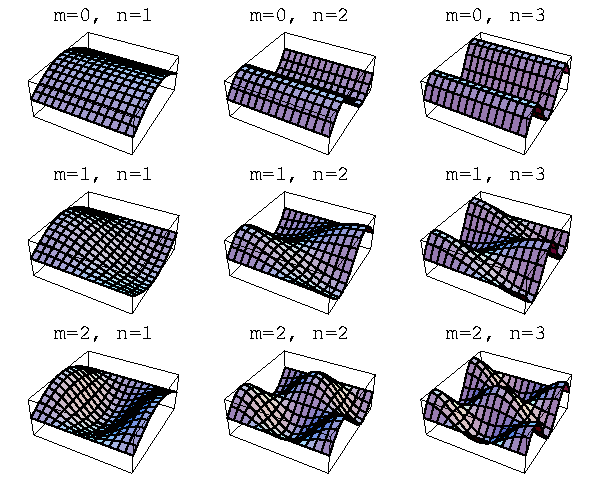
\includegraphics[width=0.6\textwidth]{pde/separation/cosmx_sinny}
    \end{center}
    \caption{The eigenfunctions.}
    \label{cosmx_sinny}
  \end{figure}

  The differential equation for $T$ becomes,
  \[
  T_{m n}' = - \left( \left( \frac{m \pi}{a} \right)^2 + \left(
      \frac{n \pi}{b} \right)^2 \right) \kappa(t) T_{m n},
  \]
  which has the solutions,
  \[
  T_{m n} =  \exp \left( - \left( \left( \frac{m \pi}{a} \right)^2 + \left(
        \frac{n \pi}{b} \right)^2 \right) \int_0^t \kappa(\tau) \,\dd \tau
  \right).
  \]
  The eigen-solutions of the partial differential equation are,
  \[
  u_{m n} =  
  \cos \left( \frac{m \pi x}{a} \right)
  \sin \left( \frac{n \pi y}{b} \right)
  \exp \left( - \left( \left( \frac{m \pi}{a} \right)^2 + \left(
        \frac{n \pi}{b} \right)^2 \right) \int_0^t \kappa(\tau) \,\dd \tau \right).
  \]
  The solution of the partial differential equation is,
  \[
  \boxed{
    u(x,y,t) = \sum_{m=0}^\infty \sum_{n=1}^\infty c_{m n}
    \cos \left( \frac{m \pi x}{a} \right)
    \sin \left( \frac{n \pi y}{b} \right)
    \exp \left( - \left( \left( \frac{m \pi}{a} \right)^2 + \left(
          \frac{n \pi}{b} \right)^2 \right) \int_0^t \kappa(\tau) \,\dd \tau \right).
    }
  \]
  We determine the coefficients from the initial condition.
  \[
  u(x,y,0) = \sum_{m=0}^\infty \sum_{n=1}^\infty c_{m n}
  \cos \left( \frac{m \pi x}{a} \right)
  \sin \left( \frac{n \pi y}{b} \right)
  = f(x,y)
  \]
  \[
  \boxed{
    c_{0 n} = \frac{2}{a b} \int_0^a \int_0^b f(x,y) \sin \left( \frac{n \pi}{b}
    \right) \,\dd y \,\dd x
    }
  \]
  \[
  \boxed{
    c_{m n} = \frac{4}{a b} \int_0^a \int_0^b f(x,y) 
    \cos \left( \frac{m \pi}{a} \right)
    \sin \left( \frac{n \pi}{b} \right) \,\dd y \,\dd x
    }
  \]
\end{Solution}






%% semi-circular rod
\begin{Solution}
  \label{solution potential semi-circular rod}
  The steady state temperature satisfies Laplace's equation, $\Delta u = 0$.
  The Laplacian in cylindrical coordinates is,
  \[
  \Delta u(r,\theta,z) = u_{r r} + \frac{1}{r} u_r + \frac{1}{r^2} 
  u_{\theta\theta} + u_{z z}.
  \]
  Because of the homogeneity in the $z$ direction, we reduce the partial 
  differential equation to,
  \[
  u_{r r} + \frac{1}{r} u_r + \frac{1}{r^2} 
  u_{\theta\theta} = 0, \quad 0 < r < 1, \quad 0 < \theta < \pi.
  \]
  The boundary conditions are,
  \[
  u(r,0) = u(r,\pi) = 0, \quad u(0,\theta) = 0, \quad u(1,\theta) = 1.
  \]
  We will solve this problem with an eigenfunction expansion.  We substitute
  the separation of variables $u(r,\theta) = R(r) T(\theta)$ into the
  partial differential equation.
  \begin{gather*}
    R'' T + \frac{1}{r} R' T + \frac{1}{r^2} R T'' = 0 \\
    r^2 \frac{R''}{R} + r \frac{R'}{R} = - \frac{T''}{T} = \lambda^2
  \end{gather*}
  We have the regular Sturm-Liouville eigenvalue problem,
  \[
  T'' = -\lambda^2 T, \quad T(0) = T(\pi) = 0,
  \]
  which has the solutions,
  \[
  \lambda_n = n, \quad
  T_n = \sin(n \theta), \quad
  n \in \mathbb{N}.
  \]
  The problem for $R$ becomes,
  \[
  r^2 R'' + r R' - n^2 R = 0, \quad R(0) = 0.
  \]
  This is an Euler equation.  We substitute $R = r^\alpha$ into the differential
  equation to obtain,
  \begin{gather*}
    \alpha (\alpha-1) + \alpha - n^2 = 0, \\
    \alpha = \pm n.
  \end{gather*}
  The general solution of the differential equation for $R$ is
  \[
  R_n = c_1 r^n + c_2 r^{-n}.
  \]
  The solution that vanishes at $r = 0$ is
  \[
  R_n = c r^n.
  \]
  The eigen-solutions of the differential equation are,
  \[
  u_n = r^n \sin(n \theta).
  \]
  The solution of the partial differential equation is
  \[
  u(r,\theta) = \sum_{n=1}^\infty a_n r^n \sin(n \theta).
  \]
  We determine the coefficients from the boundary condition at $r = 1$.
  \begin{gather*}
    u(1,\theta) = \sum_{n=1}^\infty a_n \sin(n \theta) = 1 \\
    a_n = \frac{2}{\pi} \int_0^\pi \sin(n \theta) \,\dd \theta
    = \frac{2}{\pi n} \left( 1 - (-1)^n \right)
  \end{gather*}
  The solution of the partial differential equation is
  \[
  \boxed{
    u(r,\theta) = \frac{4}{\pi} \sum_{ \substack{n = 1 \\ \mathrm{odd}\ n} }^\infty 
    r^n \sin(n \theta).
    }
  \]
\end{Solution}



%% Steady state temperature in a semi-infinite rectangular slab.
\begin{Solution}
  \label{solution heat semi-infinite rectangular slab}
  The problem is
  \begin{gather*}
    u_{x x} + u_{y y} = 0, \quad 0 < x, \quad 0 < y < 1, \\
    u(x,0) = u(x,1) = 0, \quad u(0,y) = f(y).
  \end{gather*}
  We substitute the separation of variables $u(x,y) = X(x) Y(y)$ into the 
  partial differential equation.
  \begin{gather*}
    X'' Y + X Y'' = 0 \\
    \frac{X''}{X} = - \frac{Y''}{Y} = \lambda^2
  \end{gather*}
  We have the regular Sturm-Liouville problem,
  \[
  Y'' = - \lambda^2 Y, \quad Y(0) = Y(1) = 0,
  \]
  which has the solutions,
  \[
  \lambda_n = n \pi, \quad
  Y_n = \sin(n \pi y), \quad
  n \in \mathbb{N}.
  \]
  The problem for $X$ becomes,
  \[
  X_n'' = (n \pi)^2 X,
  \]
  which has the general solution,
  \[
  X_n = c_1 \e^{n \pi x} + c_2 \e^{-n \pi x}.
  \]
  The solution that is bounded as $x \to \infty$ is,
  \[
  X_n = c \e^{-n \pi x}.
  \]
  The eigen-solutions of the partial differential equation are,
  \[
  u_n = \e^{-n \pi x} \sin(n \pi y), \quad
  n \in \mathbb{N}.
  \]
  The solution of the partial differential equation is,
  \[
  \boxed{
    u(x,y) = \sum_{n=1}^\infty a_n \e^{-n \pi x} \sin(n \pi y).
    }
  \]
  We find the coefficients from the boundary condition at $x = 0$.
  \[
  u(0,y) = \sum_{n=1}^\infty a_n \sin(n \pi y) = f(y)
  \]
  \[
  \boxed{
    a_n = 2 \int_0^1 f(y) \sin(n \pi y) \,\dd y
    }
  \]
\end{Solution}



%% Harmonic function in a sector with one inhomogeneous boundary condition.
\begin{Solution}
  \label{solution harmonic sector inhomogeneous bc}
  The Laplacian in polar coordinates is
  \[
  \Delta u \equiv u_{r r} + \frac{1}{r} u_r + \frac{1}{r^2} u_{\theta\theta}.
  \]
  Since we have homogeneous boundary conditions at $\theta = 0$ and 
  $\theta = \alpha$, we will solve this problem with an eigenfunction 
  expansion.  We substitute the separation of variables
  $u(r,\theta) = R(r) \Theta(\theta)$ into Laplace's equation.
  \begin{gather*}
    R'' \Theta + \frac{1}{r} R' \Theta + \frac{1}{r^2} R \Theta'' = 0 \\
    r^2 \frac{R''}{R} + r \frac{R'}{R} = - \frac{\Theta''}{\Theta} = \lambda^2.
  \end{gather*}
  We have a regular Sturm-Liouville eigenvalue problem for $\Theta$.
  \begin{gather*}
    \Theta'' = - \lambda^2 \Theta, \quad \Theta(0) = \Theta(\alpha) = 0
    \\
    \lambda_n = \frac{n \pi}{\alpha}, \quad
    \Theta_n = \sin \left( \frac{n \pi \theta}{\alpha} \right), \quad n \in \mathbb{Z}^+.
  \end{gather*}
  We have Euler equations for $R_n$.  We solve them with the substitution 
  $R = r^\beta$.
  \begin{gather*}
    r^2 R_n'' + r R_n' - \left( \frac{n \pi}{\alpha} \right)^2 R_n = 0, \quad R_n(a) = 0
    \\
    \beta (\beta-1) + \beta - \left( \frac{n \pi}{\alpha} \right)^2 = 0 
    \\
    \beta = \pm \frac{n \pi}{\alpha}
    \\
    R_n = c_1 r^{n \pi / \alpha} + c_2 r^{-n \pi / \alpha}.
  \end{gather*}
  The solution, (up to a multiplicative constant), that vanishes at $r = a$ is
  \[
  R_n = r^{n \pi / \alpha} - a^{2 n \pi / \alpha} r^{-n \pi / \alpha}.
  \]
  Thus the series expansion of our solution is,
  \[
  \boxed{
    u(r,\theta) = \sum_{n=1}^\infty u_n 
    \left( r^{n \pi / \alpha} - a^{2 n \pi / \alpha} r^{-n \pi / \alpha}
    \right) \sin \left( \frac{n \pi \theta}{\alpha} \right).
    }
  \]
  We determine the coefficients from the boundary condition at $r = b$.
  \begin{gather*}
    u(b,\theta) = \sum_{n=1}^\infty u_n \left( b^{n \pi / \alpha} - a^{2 n \pi / \alpha} b^{-n \pi / \alpha} \right) 
    \sin \left( \frac{n \pi \theta}{\alpha} \right) = f(\theta)
    \\
    \boxed{
      u_n = \frac{2}{\alpha \left( b^{n \pi / \alpha} - a^{2 n \pi / \alpha} b^{-n \pi / \alpha} \right)}
      \int_0^\alpha f(\theta) \sin \left( \frac{n \pi \theta}{\alpha} \right) \,\dd \theta
      }
  \end{gather*}
\end{Solution}








%% Piano string instantaneously struck.
\begin{Solution}
  \label{solution piano string instantaneously struck}
  $\phantom{a}$

  \textbf{a)}
  The mathematical statement of the problem is
  \begin{gather*}
    u_{t t} = c^2 u_{x x}, \quad 0 < x < L, \quad t > 0, \\
    u(0, t) = u(L, t) = 0, \\
    u(x, 0) = 0, \quad u_t(x, 0) = 
    \begin{cases}
      v &\mathrm{for}\ |x-\xi| < d \\
      0 &\mathrm{for}\ |x-\xi| > d.
    \end{cases}
  \end{gather*}
  Because we are interest in the harmonics of the motion,
  we will solve this problem with an eigenfunction expansion in $x$.  We 
  substitute the separation of variables $u(x, t) = X(x) T(t)$ into the wave
  equation.
  \begin{gather*}
    X T'' = c^2 X'' T \\
    \frac{ T'' }{ c^2 T } = \frac{X''}{X} = - \lambda^2
  \end{gather*}
  The eigenvalue problem for $X$ is,
  \[
  X'' = - \lambda^2 X, \quad X(0) = X(L) = 0,
  \]
  which has the solutions,
  \[
  \lambda_n = \frac{n \pi}{L}, \quad X_n = \sin\left( \frac{n \pi x}{L} \right),
  \quad n \in \mathbb{N}.
  \]
  The ordinary differential equation for the $T_n$ are,
  \[
  T_n'' = - \left( \frac{n \pi c}{L} \right)^2 T_n,
  \]
  which have the linearly independent solutions,
  \[
  \cos\left( \frac{n \pi c t}{L} \right), \quad
  \sin\left( \frac{n \pi c t}{L} \right).
  \]
  The solution for $u(x,t)$ is a linear combination of the eigen-solutions.
  \[
  u(x, t) = \sum_{n=1}^\infty \sin\left( \frac{n \pi x}{L} \right) \left(
    a_n \cos\left( \frac{n \pi c t}{L} \right)
    + b_n \sin\left( \frac{n \pi c t}{L} \right) \right)
  \]
  Since the string initially has zero displacement, each of the $a_n$ are zero.
  \[
  u(x, t) = \sum_{n=1}^\infty b_n \sin\left( \frac{n \pi x}{L} \right) 
  \sin\left( \frac{n \pi c t}{L} \right)
  \]
  Now we use the initial velocity to determine the coefficients in the expansion.
  Because the position is a continuous function of $x$, and there is a jump
  discontinuity in the velocity as a function of $x$, the coefficients in the
  expansion will decay as $1/n^2$.
  \begin{gather*}
    u_t(x, 0) = \sum_{n=1}^\infty \frac{n \pi c}{L} b_n \sin\left( \frac{n \pi x}{L}\right)
    = \begin{cases}
      v &\mathrm{for}\ |x-\xi| < d \\
      0 &\mathrm{for}\ |x-\xi| > d.
    \end{cases} \\
    \frac{n \pi c}{L} b_n = \frac{2}{L} \int_0^L u_t(x, 0) 
    \sin\left( \frac{n \pi x}{L} \right) \,\dd x
  \end{gather*}
  \begin{align*}
    b_n &= \frac{2}{n \pi c} \int_{\xi-d}^{\xi+d} v
    \sin\left( \frac{n \pi x}{L} \right) \,\dd x \\
    &= \frac{4 L v}{n^2 \pi^2 c} \sin\left( \frac{n \pi d}{L} \right)
    \sin\left( \frac{n \pi \xi}{L} \right)
  \end{align*}
  The solution for $u(x, t)$ is,
  \[
  \boxed{
    u(x, t) = \frac{4 L v}{\pi^2 c} \sum_{n=1}^\infty \frac{1}{n^2} 
    \sin\left( \frac{n \pi d}{L} \right)
    \sin\left( \frac{n \pi \xi}{L} \right)
    \sin\left( \frac{n \pi x}{L} \right)
    \sin\left( \frac{n \pi c t}{L} \right).
    }
  \]

  \textbf{b)}
  The form of the solution is again,
  \[
  u(x, t) = \sum_{n=1}^\infty b_n \sin\left( \frac{n \pi x}{L} \right) 
  \sin\left( \frac{n \pi c t}{L} \right)
  \]
  We determine the coefficients in the expansion from the initial velocity.
  \begin{gather*}
    u_t(x, 0) = \sum_{n=1}^\infty \frac{n \pi c}{L} b_n \sin\left( \frac{n \pi x}{L}\right)
    = \begin{cases}
      v \cos\left( \frac{\pi(x-\xi)}{2d} \right) &\mathrm{for}\ |x-\xi| < d \\
      0 &\mathrm{for}\ |x-\xi| > d.
    \end{cases} \\
    \frac{n \pi c}{L} b_n = \frac{2}{L} \int_0^L u_t(x, 0) 
    \sin\left( \frac{n \pi x}{L} \right) \,\dd x
  \end{gather*}
  \begin{gather*}
    b_n = \frac{2}{n \pi c} \int_{\xi-d}^{\xi+d} v 
    \cos\left( \frac{\pi(x-\xi)}{2d} \right)
    \sin\left( \frac{n \pi x}{L} \right) \,\dd x \\
    b_n = \begin{cases}
      \frac{8 d L^2 v}{n \pi^2 c (L^2 - 4 d^2 n^2)}
      \cos\left( \frac{n \pi d}{L} \right)
      \sin\left( \frac{n \pi \xi}{L} \right)
      &\mathrm{for}\ d \neq \frac{L}{2 n}, \\
      \frac{v}{n^2 \pi^2 c} \left( 2 n \pi d + L \sin\left( \frac{2 n \pi d}{L} 
        \right) \right) \sin\left( \frac{n \pi \xi}{L} \right)
      &\mathrm{for}\ d = \frac{L}{2 n}
    \end{cases}
  \end{gather*}
  The solution for $u(x, t)$ is,
  \begin{gather*}
    \boxed{
      u(x, t) = \frac{8 d L^2 v}{\pi^2 c} \sum_{n=1}^\infty \frac{1}{n (L^2 - 4 d^2 n^2)} 
      \cos\left( \frac{n \pi d}{L} \right)
      \sin\left( \frac{n \pi \xi}{L} \right)
      \sin\left( \frac{n \pi x}{L} \right)
      \sin\left( \frac{n \pi c t}{L} \right) 
      \quad \mathrm{for}\ d \neq \frac{L}{2 n},
      } \\
    \boxed{
      u(x, t) = \frac{v}{\pi^2 c} \sum_{n=1}^\infty \frac{1}{n^2}
      \left( 2 n \pi d + L \sin\left( \frac{2 n \pi d}{L} \right) \right)
      \sin\left( \frac{n \pi \xi}{L} \right)
      \sin\left( \frac{n \pi x}{L} \right)
      \sin\left( \frac{n \pi c t}{L} \right) 
      \quad \mathrm{for}\ d = \frac{L}{2 n}.
      }
  \end{gather*}

  \textbf{c)}
  The kinetic energy of the string is
  \[
  E = \frac{1}{2} \int_0^L \rho \left( u_t(x, t) \right)^2 \,\dd x,
  \]
  where $\rho$ is the density of the string per unit length.  

  \textbf{Flat Hammer.}
  The $n^{\mathrm{th}}$ harmonic is
  \[
  u_n = \frac{4 L v}{n^2 \pi^2 c} 
  \sin\left( \frac{n \pi d}{L} \right)
  \sin\left( \frac{n \pi \xi}{L} \right)
  \sin\left( \frac{n \pi x}{L} \right)
  \sin\left( \frac{n \pi c t}{L} \right).
  \]
  The kinetic energy of the $n^{\mathrm{th}}$ harmonic is
  \[
  E_n = \frac{\rho}{2} \int_0^L \left( \frac{\partial u_n}{\partial t} \right)^2 \,\dd x
  = \frac{4 L v^2}{n^2 \pi^2} 
  \sin^2\left( \frac{n \pi d}{L} \right)
  \sin^2\left( \frac{n \pi \xi}{L} \right)
  \cos^2 \left( \frac{n \pi c t}{L} \right).
  \]
  This will be maximized if
  \begin{gather*}
    \sin^2 \left( \frac{ n \pi \xi}{L} \right) = 1, \\
    \frac{n \pi \xi}{L} = \frac{\pi(2 m - 1)}{2}, \quad m = 1, \ldots, n, \\
    \boxed{
      \xi = \frac{(2 m - 1)L}{2 n}, \quad m = 1, \ldots, n
      }
  \end{gather*}
  We note that the kinetic energies of the $n^{\mathrm{th}}$ harmonic decay
  as $1/n^2$.

  \textbf{Curved Hammer.}
  We assume that $d \neq \frac{L}{2n}$.  The $n^{\mathrm{th}}$ harmonic is
  \[
  u_n = \frac{8 d L^2 v}{n \pi^2 c (L^2 - 4 d^2 n^2)}
  \cos\left( \frac{n \pi d}{L} \right)
  \sin\left( \frac{n \pi \xi}{L} \right)
  \sin\left( \frac{n \pi x}{L} \right)
  \sin\left( \frac{n \pi c t}{L} \right).
  \]
  The kinetic energy of the $n^{\mathrm{th}}$ harmonic is
  \[
  E_n = \frac{\rho}{2} \int_0^L \left( \frac{\partial u_n}{\partial t} \right)^2 \,\dd x
  = \frac{16 d^2 L^3 v^2}{ \pi^2 (L^2 - 4 d^2 n^2)^2 }
  \cos^2\left( \frac{n \pi d}{L} \right)
  \sin^2\left( \frac{n \pi \xi}{L} \right)
  \cos^2 \left( \frac{n \pi c t}{L} \right).
  \]
  This will be maximized if
  \begin{gather*}
    \sin^2 \left( \frac{ n \pi \xi}{L} \right) = 1, \\
    \boxed{
      \xi = \frac{(2 m - 1)L}{2 n}, \quad m = 1, \ldots, n
      }
  \end{gather*}
  We note that the kinetic energies of the $n^{\mathrm{th}}$ harmonic decay
  as $1/n^4$.
\end{Solution}
















%% Piano string, time dependent forcing.
\begin{Solution}
  \label{solution piano string time dependent forcing}
  In mathematical notation, the problem is
  \begin{gather*}
    u_{t t} - c^2 u_{x x} = s(x, t), \quad 0 < x < L, \quad t > 0, \\
    u(0, t) = u(L, t) = 0, \\
    u(x, 0) = u_t(x, 0) = 0.
  \end{gather*}
  Since this is an 
  inhomogeneous partial differential equation, we will expand the solution in a 
  series of eigenfunctions in $x$ for which the coefficients are functions
  of $t$.   The solution for $u$ has the form,
  \[
  u(x, t) = \sum_{n=1}^\infty u_n(t) \sin\left( \frac{n \pi x}{L} \right).
  \]
  Substituting this expression into the inhomogeneous partial differential 
  equation will give us ordinary differential equations for each of the $u_n$.  
  \[
  \sum_{n=1}^\infty \left( u_n'' + c^2 \left( \frac{n \pi}{L} \right)^2 u_n \right)
  \sin\left( \frac{n \pi x}{L} \right) = s(x, t).
  \]
  We expand the right side in a series of the eigenfunctions.
  \[
  s(x, t) = \sum_{n=1}^\infty s_n(t) \sin\left( \frac{n \pi x}{L} \right).
  \]
  For $0 < t < \delta$ we have
  \begin{align*}
    s_n(t) &= \frac{2}{L} \int_0^L s(x, t) \sin\left( \frac{n \pi x}{L} \right) 
    \,\dd x \\
    &= \frac{2}{L} \int_0^L v \cos\left( \frac{\pi(x-\xi)}{2d} \right)
    \sin\left( \frac{\pi t}{\delta} \right)
    \sin\left( \frac{n \pi x}{L} \right) \,\dd x \\
    &= \frac{8 d L v}{\pi (L^2 - 4 d^2 n^2)}
    \cos\left( \frac{n \pi d}{L} \right)
    \sin\left( \frac{n \pi \xi}{L} \right)
    \sin\left( \frac{\pi t}{\delta} \right).
  \end{align*}
  For $t > \delta$, $s_n(t) = 0$.  Substituting this into the partial 
  differential equation yields,
  \[
  u_n'' + \left( \frac{n \pi c}{L} \right)^2 u_n = 
  \begin{cases}
    \frac{8 d L v}{\pi (L^2 - 4 d^2 n^2)}
    \cos\left( \frac{n \pi d}{L} \right)
    \sin\left( \frac{n \pi \xi}{L} \right)
    \sin\left( \frac{\pi t}{\delta} \right),
    &\mathrm{for}\ t < \delta, \\
    0 &\mathrm{for}\ t > \delta.
  \end{cases}
  \]
  Since the initial position and velocity of the string is zero, we have
  \[
  u_n(0) = u_n'(0) = 0.
  \]
  First we solve the differential equation on the range $0 < t < \delta$.
  The homogeneous solutions are
  \[
  \cos\left( \frac{n \pi c t}{L} \right), \quad
  \sin\left( \frac{n \pi c t}{L} \right).
  \]
  Since the right side of the ordinary differential equation is a constant times
  $\sin(\pi t / \delta)$, which is an eigenfunction of the differential 
  operator, we can guess the form of a particular solution, $p_n(t)$.
  \[
  p_n(t) = d \sin\left( \frac{\pi t}{\delta} \right)
  \]
  We substitute this into the ordinary differential equation to determine the
  multiplicative constant $d$.
  \[
  p_n(t) = - \frac{8 d \delta^2 L^3 v}{\pi^3 (L^2 - c^2 \delta^2 n^2)
    (L^2 - 4 d^2 n^2) } \cos\left( \frac{n \pi d}{L} \right)
  \sin\left( \frac{n \pi \xi}{L} \right) 
  \sin\left( \frac{\pi t}{\delta} \right)
  \]
  The general solution for $u_n(t)$ is
  \[
  u_n(t) = a \cos\left( \frac{n \pi c t}{L} \right)
  + b \sin\left( \frac{n \pi c t}{L} \right)
  - \frac{8 d \delta^2 L^3 v}{\pi^3 (L^2 - c^2 \delta^2 n^2)
    (L^2 - 4 d^2 n^2) } \cos\left( \frac{n \pi d}{L} \right)
  \sin\left( \frac{n \pi \xi}{L} \right) 
  \sin\left( \frac{\pi t}{\delta} \right).
  \]
  We use the initial conditions to determine the constants $a$ and $b$.  The
  solution for $0 < t < \delta$ is
  \[
  u_n(t) = \frac{8 d \delta^2 L^3 v}{\pi^3 (L^2 - c^2 \delta^2 n^2)
    (L^2 - 4 d^2 n^2) } \cos\left( \frac{n \pi d}{L} \right)
  \sin\left( \frac{n \pi \xi}{L} \right) 
  \left( \frac{L}{\delta c n} \sin\left( \frac{n \pi c t}{L} \right)
    - \sin\left( \frac{\pi t}{\delta} \right) \right).
  \]
  The solution for $t > \delta$, the solution is a linear combination of
  the homogeneous solutions.  This linear combination is determined by
  the position and velocity at $t = \delta$.  We use the above solution to 
  determine these quantities.
  \begin{gather*}
    u_n(\delta) = \frac{8 d \delta^2 L^4 v}{\pi^3 \delta c n 
      (L^2 - c^2 \delta^2 n^2) (L^2 - 4 d^2 n^2) } 
    \cos\left( \frac{n \pi d}{L} \right)
    \sin\left( \frac{n \pi \xi}{L} \right) 
    \sin\left( \frac{n \pi c \delta}{L} \right) \\
    u_n'(\delta) = \frac{8 d \delta^2 L^3 v}{\pi^2 \delta (L^2 - c^2 \delta^2 n^2)
      (L^2 - 4 d^2 n^2) } \cos\left( \frac{n \pi d}{L} \right)
    \sin\left( \frac{n \pi \xi}{L} \right) 
    \left( 1 + \cos\left( \frac{n \pi c \delta}{L} \right) \right)
  \end{gather*}
  The fundamental set of solutions at $t = \delta$ is
  \[
  \left\{
    \cos\left( \frac{n \pi c(t - \delta)}{L} \right), 
    \frac{L}{n \pi c} \sin\left( \frac{n \pi c(t - \delta)}{L} \right)
  \right\}
  \]
  From the initial conditions at $t = \delta$, we see that the solution for
  $t > \delta$ is

  \begin{center}
    \fbox{
      \parbox{5.5in}{
        \begin{multline*}
          u_n(t) = \frac{8 d \delta^2 L^3 v}{\pi^3 (L^2 - c^2 \delta^2 n^2)
            (L^2 - 4 d^2 n^2) } \cos\left( \frac{n \pi d}{L} \right)
          \sin\left( \frac{n \pi \xi}{L} \right)  \\
          \left( \frac{L}{\delta c n} \sin\left( \frac{n \pi c \delta}{L} \right)
            \cos\left( \frac{n \pi c (t-\delta)}{L} \right) 
            + \frac{\pi}{\delta} \left( 1 + 
              \cos\left( \frac{n \pi c \delta}{L} \right) \right)
            \sin\left( \frac{n \pi c (t - \delta)}{L} \right) \right).
        \end{multline*}
        }
      }
  \end{center}

  \textbf{Width of the Hammer.}
  The $n^{\mathrm{th}}$ harmonic has the width dependent factor,
  \[
  \frac{d}{L^2 - 4 d^2 n^2} \cos\left( \frac{n \pi d}{L} \right).
  \]
  Differentiating this expression and trying to find zeros to determine 
  extrema would give us an equation with both algebraic and transcendental terms.
  Thus we don't attempt to find the maxima exactly.  We know that $d < L$.
  The cosine factor is large when
  \begin{gather*}
    \frac{n \pi d}{L} \approx m \pi, \quad m = 1, 2, \ldots, n-1, \\
    d \approx \frac{m L}{n}, \quad m = 1, 2, \ldots, n-1.
  \end{gather*}
  Substituting $d = m L / n$ into the width dependent factor gives us
  \[
  \frac{d}{L^2 (1 - 4 m^2)} (-1)^m.
  \]
  Thus we see that the amplitude of the $n^{\mathrm{th}}$ harmonic and hence 
  its kinetic energy will be maximized for 
  \[
  \boxed{
    d \approx \frac{L}{n}
    }
  \]
  The cosine term in the width dependent factor vanishes when
  \[
  d = \frac{(2 m - 1) L}{2 n}, \quad m = 1, 2, \ldots, n.
  \]
  The kinetic energy of the $n^{\mathrm{th}}$ harmonic is minimized for these
  widths.  

  For the lower harmonics, $n \ll \frac{L}{2d}$, the kinetic energy is 
  proportional to $d^2$; for the higher harmonics, $n \gg \frac{L}{2 d}$,
  the kinetic energy is proportional to $1 / d^2$.

  \textbf{Duration of the Blow.}
  The $n^{\mathrm{th}}$ harmonic has the duration dependent factor,
  \[
  \frac{\delta^2}{L^2 - n^2 c^2 \delta^2} \left( \frac{L}{n c \delta}
    \sin\left( \frac{n \pi c \delta}{L} \right)
    \cos\left( \frac{n \pi c (t - \delta)}{L} \right)
    + \frac{\pi}{\delta} \left( 
      1 + \cos\left( \frac{n \pi c \delta}{L} \right) \right)
    \sin\left( \frac{n \pi c (t - \delta)}{L} \right) \right).
  \]
  If we assume that $\delta$ is small, then
  \[
  \frac{L}{n c \delta} \sin\left( \frac{n \pi c \delta}{L} \right) \approx \pi.
  \]
  and
  \[
  \frac{\pi}{\delta} \left( 1 + \cos\left( \frac{n \pi c \delta}{L} \right)
  \right) \approx \frac{2 \pi}{\delta}.
  \]
  Thus the duration dependent factor is about,
  \[
  \frac{\delta}{L^2 - n^2 c^2 \delta^2} 
  \sin\left( \frac{n \pi c (t - \delta)}{L} \right).
  \]
  Thus for the lower harmonics, (those satisfying $n \ll \frac{L}{c \delta}$),
  the amplitude is proportional to $\delta$, which means that the kinetic 
  energy is proportional to $\delta^2$.  For the higher 
  harmonics, (those with $n \gg \frac{L}{c \delta}$), the amplitude is 
  proportional to $1/\delta$, which means that the kinetic energy is
  proportional to $1/\delta^2$.
\end{Solution}

















%% Propagating modes of a square waveguide.
\begin{Solution}
  \label{solution propagating modes square waveguide}
  Substituting $u(x, y, z, t) = v(x, y, z) \e^{\imath \omega t}$ into the wave 
  equation will give us a Helmholtz equation.
  \begin{gather*}
    - \omega^2 v \e^{\imath \omega t} - c^2 (v_{x x} + v_{y y} + v_{z z}) 
    \e^{\imath \omega t} = 0 \\
    v_{x x} + v_{y y} + v_{z z} + k^2 v = 0.
  \end{gather*}
  We find the propagating modes with separation of variables.  We substitute
  $v = X(x) Y(y) Z(z)$ into the Helmholtz equation.
  \begin{gather*}
    X'' Y Z + X Y'' Z + X Y Z'' + k^2 X Y Z = 0 \\
    - \frac{X''}{X} = \frac{Y''}{Y} + \frac{Z''}{Z} + k^2 = \nu^2
  \end{gather*}
  The eigenvalue problem in $x$ is
  \[
  X'' = - \nu^2 X, \quad X(0) = X(L) = 0,
  \]
  which has the solutions,
  \[
  \nu_n = \frac{n \pi}{L}, \quad X_n = \sin \left( \frac{n \pi x}{L} \right).
  \]
  We continue with the separation of variables.
  \[
  - \frac{Y''}{Y} = \frac{Z''}{Z} + k^2 - \left( \frac{n \pi}{L} \right)^2
  = \mu^2
  \]
  The eigenvalue problem in $y$ is
  \[
  Y'' = - \mu^2 Y, \quad Y(0) = Y(L) = 0,
  \]
  which has the solutions,
  \[
  \mu_n = \frac{m \pi}{L}, \quad Y_m = \sin \left( \frac{m \pi y}{L} \right).
  \]
  Now we have an ordinary differential equation for $Z$,
  \[
  Z'' + \left( k^2 - \left( \frac{\pi}{L} \right)^2 \left( n^2 + m^2 \right) 
  \right) Z = 0.
  \]
  We define the eigenvalues,
  \[
  \boxed{
    \lambda_{n,m}^2 = k^2 - \left( \frac{\pi}{L} \right)^2 \left( n^2 + m^2\right).
    }
  \]
  If $k^2 - \left( \frac{\pi}{L} \right)^2 \left( n^2 + m^2\right) < 0$, then the
  solutions for $Z$ are,
  \[
  \exp \left( \pm \sqrt{ \left( \left( \frac{\pi}{L} \right)^2 
        \left(n^2 + m^2 \right) - k^2 \right) } z \right).
  \]
  We discard this case, as the solutions are not bounded as $z \to \infty$.

  If $k^2 - \left( \frac{\pi}{L} \right)^2 \left( n^2 + m^2\right) = 0$, then the
  solutions for $Z$ are,
  \[
  \{ 1, z \}
  \]
  The solution $Z = 1$ satisfies the boundedness and nonzero condition at 
  infinity.  This corresponds to a standing wave.

  If $k^2 - \left( \frac{\pi}{L} \right)^2 \left( n^2 + m^2\right) > 0$, then the
  solutions for $Z$ are,
  \[
  \e^{\pm \imath \lambda_{n,m} z}.
  \]
  These satisfy the boundedness and nonzero conditions at infinity.
  For values of $n, m$ satisfying
  $k^2 - \left( \frac{\pi}{L} \right)^2 \left( n^2 + m^2\right) \geq 0$, there
  are the propagating modes,
  \[
  \boxed{
    u_{n,m} = \sin \left( \frac{n \pi x}{L} \right)
    \sin \left( \frac{m \pi y}{L} \right)
    \e^{\imath (\omega t \pm \lambda_{n,m} z)}.
    }
  \]
\end{Solution}


%% Rectangular drum head.  Modes of oscillation.
\begin{Solution}
  \label{solution rectangular drum head modes}
  \begin{gather}
    \label{u_tt=c^2Deltau,quad0<x<a,0<y<b}
    u_{t t} = c^2 \Delta u, \quad 0 < x < a,\ 0 < y < b, \\
    \nonumber
    u(0,y) = u(a,y) = u(x,0) = u(x,b) = 0.
  \end{gather}



  We substitute the separation of variables $u(x,y,t) = X(x) Y(y) T(t)$
  into Equation~\ref{u_tt=c^2Deltau,quad0<x<a,0<y<b}.
  \begin{gather*}
    \frac{ T'' }{ c^2 T } = \frac{ X'' }{ X } + \frac{ Y'' }{ Y }
    = - \nu \\
    \frac{ X'' }{ X } = - \frac{ Y'' }{ Y } - \nu = - \mu
  \end{gather*}
  This gives us differential equations for $X(x)$, $Y(y)$ and $T(t)$.
  \begin{gather*}
    X'' = - \mu X, \quad X(0) = X(a) = 0 \\
    Y'' = - (\nu - \mu) Y, \quad Y(0) = Y(b) = 0 \\
    T'' = - c^2 \nu T
  \end{gather*}
  First we solve the problem for $X$.
  \[
  \mu_m = \left( \frac{ m \pi }{ a } \right)^2, \quad
  X_m = \sin \left( \frac{ m \pi x }{ a } \right)
  \]
  Then we solve the problem for $Y$.
  \[
  \nu_{m,n} = \left( \frac{ m \pi }{ a } \right)^2
  + \left( \frac{ n \pi }{ b } \right)^2, \quad
  Y_{m,n} = \sin \left( \frac{ n \pi y }{ b } \right)
  \]
  Finally we determine $T$.
  \[
  T_{m,n} = \begin{matrix} \cos \\ \sin \end{matrix}
  \left( c \pi \sqrt{ \left( \frac{ m }{ a } \right)^2
      + \left( \frac{ n }{ b } \right)^2 }\, t \right)
  \]
  The modes of oscillation are
  \[
  u_{m,n} = \sin \left( \frac{ m \pi x }{ a } \right)
  \sin \left( \frac{ n \pi y }{ b } \right)
  \begin{matrix} \cos \\ \sin \end{matrix}
  \left( c \pi \sqrt{ \left( \frac{ m }{ a } \right)^2
      + \left( \frac{ n }{ b } \right)^2 }\, t \right).
  \]
  The frequencies are
  \[
  \omega_{m,n} = c \pi \sqrt{ \left( \frac{ m }{ a } \right)^2
    + \left( \frac{ n }{ b } \right)^2 }.
  \]
  Figure~\ref{sinmx_sinny} shows a few of the modes of oscillation in
  surface and density plots.
  \begin{figure}[h!]
    \begin{center}
      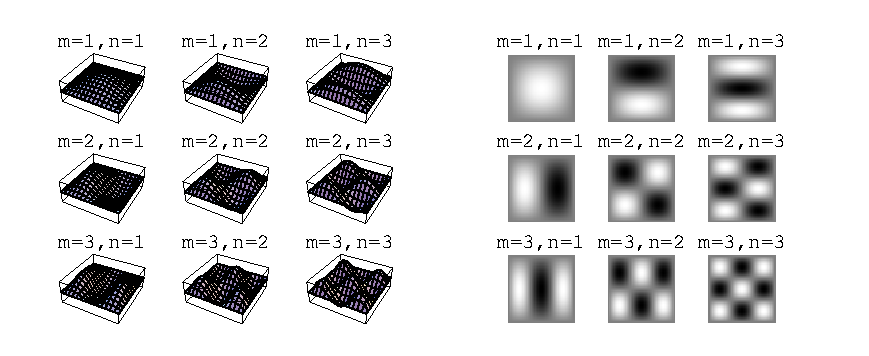
\includegraphics[width=\textwidth]{pde/separation/sinmx_sinny}
    \end{center}
    \caption{The modes of oscillation of a rectangular drum head.}
    \label{sinmx_sinny}
  \end{figure}
  %%CONTINUE solve the initial value problem.
\end{Solution}









%% \phi_t = a^2\left(\phi_{xx} + \phi_{yy}\right)
\begin{Solution}
  \label{solution separation pt=a2pxx+pyy}
  We substitute the separation of variables $\phi = X(x) Y(y) T(t)$
  into the differential equation.
  \begin{gather}
    \label{phi_t=a^2left(phi_xx+phi_yyright)}
    \phi_t = a^2 \left( \phi_{x x} + \phi_{y y} \right) \\
    \nonumber
    X Y T' = a^2 \left( X'' Y T + X Y'' T \right) \\
    \nonumber
    \frac{ T' }{ a^2 T } = \frac{ X'' }{ X } + \frac{ Y'' }{ Y } = - \nu\\
    \nonumber
    \frac{ T' }{ a^2 T } = - \nu, \quad
    \frac{ X'' }{ X } = - \nu - \frac{ Y'' }{ Y } = - \mu
  \end{gather}
  First we solve the eigenvalue problem for $X$.
  \begin{gather*}
    X'' + \mu X = 0, \quad X(0) = X(l_x) = 0 \\
    \mu_m = \left( \frac{ m \pi }{ l_x } \right)^2, \quad
    X_m(x) = \sin \left( \frac{ m \pi x }{ l_x } \right), \quad
    m \in \mathbb{Z}^+
  \end{gather*}
  Then we solve the eigenvalue problem for $Y$.
  \begin{gather*}
    Y'' + (\nu - \mu_m) Y = 0, \quad Y'(0) = Y'(l_y) = 0 \\
    \nu_{m n} = \mu_m + \left( \frac{ n \pi }{ l_y } \right)^2, \quad
    Y_{m n}(y) = \cos \left( \frac{ n \pi y }{ l_y } \right), \quad
    n \in \mathbb{Z}^{0+}
  \end{gather*}
  Next we solve the differential equation for $T$, (up to a
  multiplicative constant).
  \begin{gather*}
    T' = - a^2 \nu_{m n} T \\
    T(t) = \exp \left( - a^2 \nu_{m n} t \right)
  \end{gather*}
  The eigensolutions of Equation~\ref{phi_t=a^2left(phi_xx+phi_yyright)}
  are
  \[
  \sin(\mu_m x) \cos(\nu_{m n} y) \exp \left( - a^2 \nu_{m n} t \right),
  \quad m \in \mathbb{Z}^+,\ n \in \mathbb{Z}^{0+}.
  \]
  We choose the eigensolutions $\phi_{m n}$ to be orthonormal on
  the $xy$ domain at $t = 0$.
  \begin{gather*}
    \phi_{m 0}(x,y,t) = \sqrt{ \frac{ 2 }{ l_x l_y } }
    \sin(\mu_m x) \exp \left( - a^2 \nu_{m n} t \right),
    \quad m \in \mathbb{Z}^+ \\
    \phi_{m n}(x,y,t) = \frac{ 2 }{ \sqrt{ l_x l_y } }
    \sin(\mu_m x) \cos(\nu_{m n} y) \exp \left( - a^2 \nu_{m n} t \right),
    \quad m \in \mathbb{Z^+},\ n \in \mathbb{Z}^+
  \end{gather*}
  The solution of Equation~\ref{phi_t=a^2left(phi_xx+phi_yyright)}
  is a linear combination of the eigensolutions.
  \[
  \phi(x,y,t) = \sum_{\substack{m = 1\\n = 0}}^\infty 
  c_{m n} \phi_{m n}(x,y,t)
  \]
  We determine the coefficients from the initial condition.
  \begin{gather*}
    \phi(x,y,0) = 1 \\
    \sum_{\substack{m = 1\\n = 0}}^\infty c_{m n} \phi_{m n}(x,y,0) = 1 \\
    c_{m n} = \int_0^{l_x} \int_0^{l_y} \phi_{m n}(x,y,0) \,\dd y \,\dd x \\
    c_{m 0} = \sqrt{ \frac{ 2 }{ l_x l_y } } \int_0^{l_x} \int_0^{l_y} 
    \sin(\mu_m x) \,\dd y \,\dd x \\
    c_{m 0} = \sqrt{ 2 l_x l_y } \, \frac{ 1 - (-1)^m }{ m \pi },
    \quad m \in \mathbb{Z^+} \\
    c_{m n} = \frac{ 2 }{ \sqrt{ l_x l_y } }\int_0^{l_x} \int_0^{l_y}  
    \sin(\mu_m x) \cos(\nu_{m n} y) \,\dd y \,\dd x \\
    c_{m n} = 0, \quad m \in \mathbb{Z^+},\ n \in \mathbb{Z}^+ \\
    \phi(x,y,t) = \sum_{m = 1}^\infty c_{m 0} \phi_{m 0}(x,y,t) \\
    \boxed{
      \phi(x,y,t) = \sum_{\substack{m = 1\\ \mathrm{odd}\ m}}^\infty 
      \frac{ 2 \sqrt{ 2 l_x l_y } }{ m \pi }
      \sin(\mu_m x) \exp \left( - a^2 \nu_{m n} t \right)
      }
  \end{gather*}

  \textbf{Addendum.}
  Note that an equivalent problem to the one specified is
  \begin{gather*}
    \phi_t = a^2 \left( \phi_{x x} + \phi_{y y} \right), \quad
    0 < x < l_x,\ -\infty < y < \infty, \\
    \phi(x,y,0) = 1, \quad \phi(0,y,t) = \phi(l_y,y,t) = 0.
  \end{gather*}
  Here we have done an even periodic continuation of the problem in the
  $y$ variable.  Thus the boundary conditions 
  \[
  \phi_y(x,0,t) = \phi_y(x,l_y,t) = 0
  \]
  are automatically satisfied.  Note that this problem does not depend 
  on $y$.  Thus we only had to solve
  \begin{gather*}
    \phi_t = a^2 \phi_{x x} , \quad
    0 < x < l_x \\
    \phi(x,0) = 1, \quad \phi(0,t) = \phi(l_y,t) = 0.
  \end{gather*}
\end{Solution}







%% Using polar coordinates and separation of variables solve the heat equation.
\begin{Solution}
  \label{solution heat polar separation}
  \begin{enumerate}
    %%
    %%
  \item
    Since the initial and boundary conditions do not depend on $\theta$,
    neither does $\phi$.  We apply the separation of variables
    $\phi = u(r) T(t)$.
    \begin{gather}
      \label{phi_t=a^2Deltaphi}
      \phi_t = a^2 \Delta \phi \\
      \phi_t = a^2 \frac{1}{r} \left( r \phi_r \right)_r \\
      \frac{ T' }{ a^2 T } = \frac{1}{r} ( r u' )' = - \lambda
    \end{gather}
    We solve the eigenvalue problem for $u(r)$.
    \begin{gather*}
      (r u')' + \lambda u = 0, \quad u(0)\ \mathrm{bounded}, 
      \quad u(R) = 0 \\
      \intertext{First we write the general solution.}
      u(r) = c_1 J_0 \left( \sqrt{\lambda} r \right) + 
      c_2 Y_0 \left( \sqrt{\lambda} r \right) \\
      \intertext{The Bessel function of the second kind, $Y_0$, is not
        bounded at $r = 0$, so $c_2 = 0$.  We use the boundary
        condition at $r = R$ to determine the eigenvalues.}
      \lambda_n = \left( \frac{ j_{0,n} }{ R } \right)^2, \quad
      u_n(r) = c J_0 \left( \frac{ j_{0,n} r }{ R } \right)
    \end{gather*}
    We choose the constant $c$ so that the eigenfunctions are orthonormal
    with respect to the weighting function $r$.
    \begin{align*}
      u_n(r) &= \frac{ J_0 \left( \frac{ j_{0,n} r }{ R } \right) }
      { \sqrt{ \int_0^R r J_0^2 \left( \frac{ j_{0,n} r }{ R }
          \right) } } \\
      &= \frac{ \sqrt{2} }{ R J_1( j_{0,n} ) }
      J_0 \left( \frac{ j_{0,n} r }{ R } \right)
    \end{align*}

    Now we solve the differential equation for $T$.
    \begin{gather*}
      T' = - a^2 \lambda_n T \\
      T_n = \exp \left( - \left( \frac{ a j_{0,n} }{ R^2 } \right)^2 t \right)
    \end{gather*}

    The eigensolutions of Equation~\ref{phi_t=a^2Deltaphi} are
    \[
    \phi_n(r,t) = \frac{ \sqrt{2} }{ R J_1( j_{0,n} ) }
    J_0 \left( \frac{ j_{0,n} r }{ R } \right)
    \exp \left( - \left( \frac{ a j_{0,n} }{ R^2 } \right)^2 t \right)
    \]
    The solution is a linear combination of the eigensolutions.
    \[
    \phi = \sum_{n=1}^\infty c_n \frac{ \sqrt{2} }{ R J_1( j_{0,n} ) }
    J_0 \left( \frac{ j_{0,n} r }{ R } \right)
    \exp \left( - \left( \frac{ a j_{0,n} }{ R^2 } \right)^2 t \right)
    \]
    We determine the coefficients from the initial condition.
    \begin{gather*}
      \phi(r,\theta,0) = V \\
      \sum_{n=1}^\infty c_n \frac{ \sqrt{2} }{ R J_1( j_{0,n} ) }
      J_0 \left( \frac{ j_{0,n} r }{ R } \right) = V \\
      c_n = \int_0^R V r \frac{ \sqrt{2} }{ R J_1( j_{0,n} ) }
      J_0 \left( \frac{ j_{0,n} r }{ R } \right) \,\dd r \\
      c_n = V \frac{ \sqrt{2} }{ R J_1( j_{0,n} ) } 
      \frac{ R }{ j_{0,n} / R } 
      J_1 \left( j_{0,n} \right) \\
      c_n = \frac{ \sqrt{2}\ V R }{ j_{0,n} } \\
      \boxed{
        \phi(r,\theta,t) = 2 V \sum_{n=1}^\infty 
        \frac{ J_0 \left( \frac{ j_{0,n} r }{ R } \right) }
        { j_{0,n} J_1( j_{0,n} ) }
        \exp \left( - \left( \frac{ a j_{0,n} }{ R^2 } \right)^2 t \right)
        }
    \end{gather*}
    %%
    %%
  \item
    \begin{gather*}
      J_\nu(r) \sim \sqrt{ \frac{ 2 }{ \pi r } }\, \cos \left(
        r - \frac{\pi \nu}{2} - \frac{\pi}{4} \right), \quad
      r \to +\infty \\
      j_{\nu,n} \sim \left( n + \frac{\nu}{2} - \frac{1}{4} \right) \pi
    \end{gather*}
    For large $n$, the terms in the series solution at $t = 0$ are
    \begin{align*}
      \frac{ J_0 \left( \frac{ j_{0,n} r }{ R } \right) }
      { j_{0,n} J_1( j_{0,n} ) }
      &\sim \frac{ \sqrt{ \frac{ 2 R }{ \pi j_{0,n} r } } \cos \left(
          \frac{ j_{0,n} r }{ R } - \frac{\pi}{4} \right) }
      { j_{0,n} \sqrt{ \frac{ 2 }{ \pi j_{0,n} } }\, \cos \left(
          j_{0,n} - \frac{3 \pi}{4} \right) } \\
      &\sim \frac{ R }{ r (n - 1/4) \pi }
      \frac{ \cos \left( \frac{ (n - 1/4) \pi r }{ R } 
          - \frac{\pi}{4} \right) }
      { \cos \left( (n - 1) \pi \right) }.
    \end{align*}
    The coefficients decay as $1/n$.
  \end{enumerate}
\end{Solution}






%% Consider the solution of the diffusion equation in spherical coordinates.
\begin{Solution}
  \label{solution diffusion spherical separation}
  \begin{enumerate}
    %%
    %%
  \item
    We substitute the separation of variables 
    $\Psi = T(t) \Theta(\theta) \Phi(\phi)$ into 
    Equation~\ref{fpdfracPsit=fraca^2R^2left(frac1sintheta}
    \begin{gather*}
      T' \Theta \Phi = \frac{a^2}{R^2} \left( 
        \frac{1}{\sin \theta} \frac{\partial}{\partial \theta} 
        ( \sin \theta\, T \Theta' \Phi )
        + \frac{1}{\sin^2 \theta} T \Theta \Phi'' \right) \\
      \frac{ R^2 T' }{ a^2 T } = \left( \frac{1}{\sin \theta\, \Theta } 
        ( \sin \theta\, \Theta' )'
        + \frac{1}{\sin^2 \theta} \frac{ \Phi'' }{\Phi} \right) 
      = - \mu \\
      \frac{\sin \theta}{\Theta } 
      ( \sin \theta\, \Theta' )'
      + \mu \sin^2 \theta 
      = - \frac{ \Phi'' }{\Phi} = \nu \\
      \intertext{We have differential equations for each of $T$, $\Theta$
        and $\Phi$.}
      T' = - \mu \frac{a^2}{R^2} T, \quad
      \frac{1}{\sin \theta} ( \sin \theta\, \Theta' )'
      + \left(\mu - \frac{\nu}{\sin^2 \theta} \right) \Theta = 0, \quad
      \Phi'' + \nu \Phi = 0
    \end{gather*}
    %%
    %%
  \item
    In order that the solution be continuously differentiable, we need the
    periodic boundary conditions
    \[
    \Phi(0) = \Phi(2 \pi), \quad \Phi'(0) = \Phi'(2 \pi).
    \]
    The eigenvalues and eigenfunctions for $\Phi$ are
    \[
    \nu_n = n^2, \quad \Phi_n = \frac{1}{\sqrt{2 \pi}} \e^{\imath n \phi},
    \quad n \in \mathbb{Z}.
    \]
    Now we deal with the equation for $\Theta$.
    \begin{gather*}
      x = \cos \theta, \quad \Theta(\theta) = P(x), \quad
      \sin^2 \theta = 1 - x^2, \quad
      \frac{\dd}{\dd x} = \frac{1}{\sin \theta} \frac{\dd}{\dd \theta} \\
      \frac{1}{\sin \theta} ( \sin^2 \theta \frac{1}{\sin \theta}\, \Theta' )'
      + \left(\mu - \frac{\nu}{\sin^2 \theta} \right) \Theta = 0 \\
      \left( \left( 1 - x^2 \right) P' \right)' 
      + \left(\mu - \frac{n^2}{1 - x^2} \right) P = 0
    \end{gather*}
    $P(x)$ should be bounded at the endpoints, $x = -1$ and $x = 1$.
    %%
    %%
  \item
    If the solution does not depend on $\theta$, then the only one of 
    the $\Phi_n$ that will appear in the solution is 
    $\Phi_0 = 1 / \sqrt{2 \pi}$.  The equations for $T$ and $P$ 
    become
    \begin{gather*}
      \left( \left( 1 - x^2 \right) P' \right)' + \mu P = 0,\quad
      P(\pm 1)\ \mathrm{bounded}, \\
      T' = - \mu \frac{a^2}{R^2} T.
    \end{gather*}
    The solutions for $P$ are the Legendre polynomials.
    \[
    \mu_l = l(l+1), \quad P_l(\cos \theta), \quad l \in \mathbb{Z}^{0+}
    \]
    We solve the differential equation for $T$.
    \begin{gather*}
      T' = - l(l+1) \frac{a^2}{R^2} T \\
      T_l = \exp \left( - \frac{a^2 l(l+1)}{R^2} t \right)
    \end{gather*}
    The eigensolutions of the partial differential equation are
    \[
    \Psi_l = P_l(\cos \theta) \exp \left( - \frac{a^2 l(l+1)}{R^2} t \right).
    \]
    The solution is a linear combination of the eigensolutions.
    \[
    \Psi = \sum_{l=0}^\infty A_l P_l(\cos \theta) 
    \exp \left( - \frac{a^2 l(l+1)}{R^2} t \right)
    \]
    %%
    %%
  \item
    We determine the coefficients in the expansion from the initial 
    condition.
    \begin{gather*}
      \Psi(\theta,0) = 2 \cos^2 \theta - 1 \\
      \sum_{l=0}^\infty A_l P_l(\cos \theta) = 2 \cos^2 \theta - 1 \\
      A_0 + A_1 \cos \theta 
      + A_2 \left( \frac{3}{2} \cos^2 \theta - \frac{1}{2} \right)
      + \cdots = 2 \cos^2 \theta - 1 \\
      A_0 = - \frac{1}{3}, \quad A_1 = 0, \quad
      A_2 = \frac{4}{3}, \quad A_3 = A_4 = \cdots = 0 \\
      \Psi(\theta,t) = - \frac{1}{3} P_0(\cos \theta) 
      + \frac{4}{3} P_2(\cos \theta) 
      \exp \left( - \frac{6 a^2}{R^2} t \right) \\
      \boxed{
        \Psi(\theta,t) = - \frac{1}{3}
        + \left( 2 \cos^2 \theta - \frac{2}{3} \right)
        \exp \left( - \frac{6 a^2}{R^2} t \right)
        }
    \end{gather*}
  \end{enumerate}
\end{Solution}












%% Laplace's equation: with about 1\% (also 0.1\%) accuracy.
\begin{Solution}
  \label{solution laplace 1 percent}
  Since we have homogeneous boundary conditions at $x = 0$ and $x = 1$,
  we will expand the solution in a series of eigenfunctions in $x$.  We
  determine a suitable set of eigenfunctions with the separation of
  variables, $\phi = X(x) Y(y)$.
  \begin{gather}
    \label{phi_xx+phi_yy=0}
    \phi_{xx} + \phi_{yy} = 0 \\
    \nonumber
    \frac{ X'' }{ X } = - \frac{ Y'' }{ Y } = - \lambda
  \end{gather}
  We have differential equations for $X$ and $Y$.
  \begin{gather*}
    X'' + \lambda X = 0, \quad X(0) = X(1) = 0 \\
    Y'' - \lambda Y = 0, \quad Y(0) = 0
  \end{gather*}
  The eigenvalues and orthonormal eigenfunctions for $X$ are
  \[
  \lambda_n = (n \pi)^2, \quad X_n(x) = \sqrt{2} \sin(n \pi x),
  \quad n \in \mathbb{Z}^+.
  \]
  The solutions for $Y$ are, (up to a multiplicative constant),
  \[
  Y_n(y) = \sinh(n \pi y).
  \]
  The solution of Equation~\ref{phi_xx+phi_yy=0} is a linear combination
  of the eigensolutions.
  \[
  \phi(x,y) = \sum_{n=1}^\infty a_n \sqrt{2} \sin(n \pi x) \sinh(n \pi y)
  \]
  We determine the coefficients from the boundary condition at $y = 2$.
  \begin{gather*}
    x(1-x) = \sum_{n=1}^\infty a_n \sqrt{2} \sin(n \pi x) \sinh(n \pi 2) \\
    a_n \sinh(2 n \pi) = \sqrt{2} \int_0^1 x(1-x) \sin(n \pi x) \,\dd x \\
    a_n = \frac{ 2 \sqrt{2} (1 - (-1)^n) }{ n^3 \pi^3 \sinh(2 n \pi) } \\
    \boxed{
      \phi(x,y) = \frac{8}{\pi^3} \sum_{\substack{n = 1 \\ \mathrm{odd}\ n}}^\infty
      \frac{ 1 }{ n^3 } \sin(n \pi x) 
      \frac{ \sinh(n \pi y) }{ \sinh(2 n \pi) }
      }
  \end{gather*}
  The solution at $x = 1/2$, $y = 1$ is
  \[
  \phi(1/2,1) = - \frac{8}{\pi^3} \sum_{\substack{n = 1 \\ \mathrm{odd}\ n}}^\infty
  \frac{ 1 }{ n^3 } 
  \frac{ \sinh(n \pi) }{ \sinh(2 n \pi) }.
  \]
  Let $R_k$ be the relative error at that point incurred by taking $k$ terms.
  \begin{gather*}
    R_k = \left| 
      \frac{ - \frac{8}{\pi^3} 
        \sum_{\substack{n = k+2 \\ \mathrm{odd}\ n}}^\infty
        \frac{ 1 }{ n^3 } 
        \frac{ \sinh(n \pi) }{ \sinh(2 n \pi) } }
      {- \frac{8}{\pi^3} 
        \sum_{\substack{n = 1 \\ \mathrm{odd}\ n}}^\infty
        \frac{ 1 }{ n^3 } 
        \frac{ \sinh(n \pi) }{ \sinh(2 n \pi) } } 
    \right| \\
    R_k =   \frac{ \sum_{\substack{n = k+2 \\ \mathrm{odd}\ n}}^\infty
      \frac{ 1 }{ n^3 } 
      \frac{ \sinh(n \pi) }{ \sinh(2 n \pi) } }
    { \sum_{\substack{n = 1 \\ \mathrm{odd}\ n}}^\infty
      \frac{ 1 }{ n^3 } 
      \frac{ \sinh(n \pi) }{ \sinh(2 n \pi) } } 
  \end{gather*}
  Since $R_1 \approx 0.0000693169$ we see that one term is sufficient
  for $1\%$ or $0.1\%$ accuracy.

  Now consider $\phi_x(1/2,1)$.
  \begin{gather*}
    \phi_x(x,y) = \frac{8}{\pi^2} \sum_{\substack{n = 1 \\ \mathrm{odd}\ n}}^\infty
    \frac{ 1 }{ n^2 } \cos(n \pi x) 
    \frac{ \sinh(n \pi y) }{ \sinh(2 n \pi) } \\
    \phi_x(1/2,1) = 0
  \end{gather*}
  Since all the terms in the series are zero, accuracy is not an issue.
\end{Solution}





%% Laplace's equation: spherical coordinates, two regions.
\begin{Solution}
  \label{solution laplace spherical two regions}
  The solution has the form
  \[
  \psi = \begin{cases}
    \alpha r^{-n-1} P_n^m (\cos \theta) \sin(m \phi), &r > a \\
    \beta r^n P_n^m (\cos \theta) \sin(m \phi), &r < a.
  \end{cases}
  \]
  The boundary condition on $\psi$ at $r = a$ gives us the constraint
  \begin{gather*}
    \alpha a^{-n-1} - \beta a^n = 0 \\
    \beta = \alpha a^{-2n-1}.
  \end{gather*}
  Then we apply the boundary condition on $\psi_r$ at $r = a$.
  \begin{gather*}
    -(n+1) \alpha a^{-n-2} - n \alpha a^{-2n-1} a^{n-1} = 1 \\
    \alpha = - \frac{ a^{n+2} }{ 2n+1 } \\
    \boxed{
      \psi = \begin{cases}
        - \frac{ a^{n+2} }{ 2n+1 } r^{-n-1} 
        P_n^m (\cos \theta) \sin(m \phi), &r > a \\
        - \frac{ a^{-n+1} }{ 2n+1 } r^n 
        P_n^m (\cos \theta) \sin(m \phi), &r < a
      \end{cases}
      }
  \end{gather*}
\end{Solution}





%% Obtain a formula analogous to the Poisson formula to solve Neumann problem.
\begin{Solution}
  \label{solution poisson formula neumann}
  We expand the solution in a Fourier series.
  \[
  \phi = \frac{1}{2} a_0(r) 
  + \sum_{n=1}^\infty a_n(r) \cos(n \theta)
  + \sum_{n=1}^\infty b_n(r) \sin(n \theta)
  \]
  We substitute the series into the Laplace's equation to determine
  ordinary differential equations for the coefficients.
  \begin{gather*}
    \frac{\partial}{\partial r} \left( r \frac{\partial \phi}{\partial r} \right)
    + \frac{1}{r^2} \frac{\partial^2 \phi}{\partial \theta^2} = 0 \\
    a_0'' + \frac{1}{r} a_0' = 0, \quad
    a_n'' + \frac{1}{r} a_n' - n^2 a_n = 0, \quad
    b_n'' + \frac{1}{r} b_n' - n^2 b_n = 0
  \end{gather*}
  The solutions that are bounded at $r = 0$ are, (to within
  multiplicative constants),
  \[
  a_0(r) = 1, \quad a_n(r) = r^n, \quad b_n(r) = r^n.
  \]
  Thus $\phi(r,\theta)$ has the form
  \[
  \phi(r,\theta) = \frac{1}{2} c_0 
  + \sum_{n=1}^\infty c_n r^n \cos(n \theta)
  + \sum_{n=1}^\infty d_n r^n \sin(n \theta)
  \]
  We apply the boundary condition at $r = R$.
  \[
  \phi_r(R,\theta) = \sum_{n=1}^\infty n c_n R^{n-1} \cos(n \theta)
  + \sum_{n=1}^\infty n d_n R^{n-1} \sin(n \theta) 
  \]
  In order that $\phi_r(R,\theta)$ have a Fourier series of this form,
  it is necessary that
  \[
  \int_0^{2 \pi} \phi_r(R,\theta) \,\dd \theta = 0.
  \]
  In that case $c_0$ is arbitrary in our solution.
  The coefficients are
  \begin{gather*}
    c_n = \frac{1}{\pi n R^{n-1}} \int_0^{2 \pi} \phi_r(R,\alpha) 
    \cos(n \alpha) \,\dd \alpha, \quad
    d_n = \frac{1}{\pi n R^{n-1}} \int_0^{2 \pi} \phi_r(R,\alpha) 
    \sin(n \alpha) \,\dd \alpha.
  \end{gather*}
  We substitute the coefficients into our series solution to determine
  it up to the additive constant.
  \begin{gather*}
    \phi(r,\theta) = \frac{R}{\pi} \sum_{n=1}^\infty \frac{1}{n}
    \left( \frac{r}{R} \right)^n \int_0^{2 \pi} 
    \phi_r(R,\alpha) \cos(n (\theta-\alpha)) \,\dd \alpha \\
    \phi(r,\theta) = \frac{R}{\pi} \int_0^{2 \pi} \phi_r(R,\alpha) 
    \sum_{n=1}^\infty \frac{1}{n} \left( \frac{r}{R} \right)^n 
    \cos(n (\theta-\alpha)) \,\dd \alpha \\
    \phi(r,\theta) = \frac{R}{\pi} \int_0^{2 \pi} \phi_r(R,\alpha) 
    \sum_{n=1}^\infty \int_0^r \frac{\rho^{n-1}}{R^n} \,\dd \rho
    \Re \left( \e^{\imath n (\theta-\alpha)} \right) \,\dd \alpha \\
    \phi(r,\theta) = \frac{R}{\pi} \int_0^{2 \pi} \phi_r(R,\alpha) 
    \Re \left( \int_0^r \frac{1}{\rho} \sum_{n=1}^\infty
      \frac{\rho^n}{R^n} \e^{\imath n (\theta-\alpha)} \,\dd \rho
    \right) \,\dd \alpha \\
    \phi(r,\theta) = \frac{R}{\pi} \int_0^{2 \pi} \phi_r(R,\alpha) 
    \Re \left( \int_0^r \frac{1}{\rho} 
      \frac{ \frac{\rho}{R} \e^{\imath (\theta - \alpha)} }
      { 1 - \frac{\rho}{R} \e^{\imath (\theta - \alpha)} }
      \,\dd \rho \right) \,\dd \alpha \\
    \phi(r,\theta) = - \frac{R}{\pi} \int_0^{2 \pi} \phi_r(R,\alpha) 
    \Re \left( \ln \left( 1 - \frac{r}{R} \e^{\imath (\theta - \alpha)}
      \right) \right) \,\dd \alpha \\
    \phi(r,\theta) = - \frac{R}{\pi} \int_0^{2 \pi} \phi_r(R,\alpha) 
    \ln \left| 1 - \frac{r}{R} \e^{\imath (\theta - \alpha)}
    \right| \,\dd \alpha \\
    \boxed{
      \phi(r,\theta) = - \frac{R}{2 \pi} \int_0^{2 \pi} \phi_r(R,\alpha) 
      \ln \left( 1 - 2 \frac{r}{R} \cos(\theta - \alpha)
        + \frac{r^2}{R^2} \right) \,\dd \alpha 
      }
  \end{gather*}
\end{Solution}








%% Investigate solutions of \[\phi_t = a^2 \phi_{x x}\]
\begin{Solution}
  \label{solution separation pt=a2pxx}
  We will assume that both $\alpha$ and $\beta$ are nonzero.  The cases
  of real and pure imaginary have already been covered.
  We solve the ordinary differential equations, (up to a multiplicative
  constant), to find special solutions of the diffusion equation.
  \begin{gather*}
    \frac{T'}{T} = (\alpha + \imath \beta)^2, \quad
    \frac{X''}{X} = \frac{(\alpha + \imath \beta)^2}{a^2} \\
    T = \exp \left( (\alpha + \imath \beta)^2 t \right), \quad
    X = \exp \left( \pm \frac{\alpha + \imath \beta}{a} x \right) \\
    T = \exp \left( \left(\alpha^2 - \beta^2 \right) t 
      + \imath 2 \alpha \beta t \right), \quad
    X = \exp \left( \pm \frac{\alpha}{a} x  
      \pm \imath \frac{\beta}{a} x \right) \\
    \phi = \exp \left( \left(\alpha^2 - \beta^2 \right) t \pm \frac{\alpha}{a} x 
      + \imath \left( 2 \alpha \beta t \pm \frac{\beta}{a} x \right) \right) \\
    \intertext{We take the sum and difference of these solutions to obtain}
    \boxed{
      \phi = \exp \left( \left(\alpha^2 - \beta^2 \right) t 
        \pm \frac{\alpha}{a} x \right)
      \begin{matrix} \cos \\ \sin \end{matrix}
      \left( 2 \alpha \beta t \pm \frac{\beta}{a} x \right)
      }
  \end{gather*}
\end{Solution}




\raggedbottom
}
